% ===================================================================
% Arquivo: capitulos/parte-III-pilares/cap-10-perda-binaria.tex
% ===================================================================

\chapter{Funções de perda para regressão}%
\label{cap:perda-regressao}

Agora agora vimos o funcionamento da retropropagação, e como ela faz uso dos otimizadores, os quais funcionam como um barco, percorrendo as ondas em busca dos pontos de mínimo. Além disso, foram vistas em seguida diversas funções de ativação, começando pelas sigmoidais. Depois pelas retificadoras, e por fim uma coletânea de diferentes funções. Contudo, está na hora de entender um outro lado da retropropagação: as funções de perda, as quais são justamente as ondas que os otimizadores percorrem.

Esse capítulo explica alguns dos diferentes tipos de funções de perda, mais precisamente as funções de perda para tarefas de regressão. Portanto, o capítulo pode ser dividido em quatro grandes partes: funções de perda para propósitos gerais, funções de perda para medir o erro relativo, funções que vão além do cálculo da média dos erros. Por último, funções que são utilizadas para problemas que seguem outros tipos de distribuição (como as distribuições de Poisson e Gamma).

Para explicar cada uma das funções é apresentado as suas equações, os gráficos (contendo as vistas em duas e três dimensões), as derivadas parciais junto com os seus respectivos gráficos. Além disso, ao final de cada explicação dessas funções, é selecionado uma série de artigos que exploram o uso dessas funções para resolver problemas variados em aprendizado de máquina. Já no final do capítulo, está uma tabela resumo, explicando as principais características das funções e seus usos. Também é dedicada uma seção que apresenta um diagrama, que serve de guia para escolher a função de perda ideal para um problema de regressão.

\section{Exemplo ilustrativo: jogando dardos}

Pense que você está jogando dardos com seus amigos, e, quer decidir quem está com mais pontos. Mas, você não está satisfeito em considerar as marcações que estão no jogo, e, decidiu inovar. Assim, você pegou uma régua e passou a medir a distância que os dardos que você e seus amigos haviam jogado no centro. Quem chegasse mais próximo do centro, ganhava o jogo.

Essa ideia de medir o quão próximo você está do resultado desejado utilizando a distância entre esses dois pontos como parâmetro, é o motivador pela criação das funções de perda para regressão. Essas funções utilizam diferentes fórmulas, com todas com o mesmo intuito, medir a distância em que a predição dado pelo modelo está do ponto real (desejado).

\section{Características das funções de perda}

Antes de discutir as funções de perda para tarefas de regressão, é importante citar as principais propriedades que uma função de perda, seja ela para tarefas de regressão ou para outros tipos de tarefa. Em \textit{Loss Functions and Metrics in Deep Learning}, \textcite{LossesArticle} explicam algumas características desse grupo de funções. Os autores argumentam que algumas propriedades das funções de perda são: \textbf{convexidade}, \textbf{diferenciabilidade}, \textbf{robustez}, \textbf{suavidade}, \textbf{esparsidade} e \textbf{monotonicidade} \parencite{LossesArticle}. Todas essas propriedades devem ser consideradas ao escolher a função de perda ideal para resolver um determinado tipo de problema.

\begin{description}[style=unboxed, leftmargin=0cm, font=\bfseries]
    
    \item[Convexidade:] 
    Uma função convexa é uma função na qual qual ponto de mínimo local é também o ponto de mínimo global \parencite{LossesArticle}. Uma forma fácil de identificar se uma função é convexa ou não, é verificar se ela possui o formato de um funil, ou um formato da letra ``V''. Em \textit{Convex optimization}, \textcite{boyd2004convex} elaboram e discutem uma série de teoremas que buscam avaliar se uma função estudada é convexa ou não. Alguns desses teoremas são utilizados no Apêndice~\ref{apendice:propriedades-analiticas-funcoes-de-perda} (Propriedades Analíticas das Funções de Perda) para provar a convexidade das funções de perda analisadas durante este e outros capítulos.

    Funções convexas são ideais para serem utilizadas como funções de perda, porque facilitam a otimização utilizando métodos baseados em gradiente. Como foi visto no Capítulo~\ref{cap:retropropagacao-gradiente}, é bem mais intuitivo para o modelo encontrar pontos de mínimo em uma função que apresenta o formato de uma tigela do que em uma função não-convexa, cheia de ondas e com vários pontos de mínimo locais.
    
    \item[Diferenciabilidade:] 
    A questão da diferenciabilidade está relacionada também com a utilização de otimizadores baseados em gradiente. Ao utilizar a retropropagação para fazer o ajuste de parâmetros, o primeiro cálculo do gradiente será pelas derivadas parciais da função de perda. Essas derivadas formam juntas o vetor gradiente que será propagado por toda a rede, das camadas mais próximas da saída até as camadas mais próximas da entrada. De tal maneira que vai sendo ajustado os valores dos pesos e vieses do modelo. 

    Utilizar uma função que não seja diferenciável ou que possuam muitos pontos de descontinuidade certamente irá afetar negativamente o algoritmo da retropropagação, atrapalhando o aprendizado com o uso do gradiente\footnote{Vale dizer também que mesmo que uma função apresente um ou outro ponto de descontinuidade, pode ser que isso não atrapalhe a otimização por gradiente, um exemplo disso é a função erro absoluto médio, que a apresenta um ponto de descontinuidade. Mas, é possível contornar esse ``problema'' utilizando o cálculo do subgradiente.}.

    Em \textit{Principles of Mathematical Analysis}, \textcite{rudin1976principles} discute a notação de classes de continuidade, chamadas neste livro por $C^k$, para descrever o comportamento de funções matemáticas. Uma função de classe $C^0$ é uma função contínua em todo o seu domínio, mas não é suave, de fato que sua derivada não será contínua. Uma função de classe $C^1$ é contínua e suave em todo o seu domínio, mas a derivada de sua derivada não é contínua. Por fim, uma função de classe $C^{\infty}$ (infinitamente diferenciável), tem todas as suas derivadas contínuas.

    A notação de classes de continuidade nos ajuda a entender de forma mais fácil as propriedades de uma função. Neste livro, para cada uma das funções de perda analisadas, é discutida a sua classe de continuidade. Suas provas matemáticas são encontradas no Apêndice~\ref{apendice:propriedades-analiticas-funcoes-de-perda}.
    
    \item[Robustez:] 
    As funções de perda devem ser capazes de lidar com \textit{outliers} e não serem afetadas por um pequeno número de valores extremos \parencite{LossesArticle}. Os \textit{outliers} são valores que estão fora da padrão dos dados gerais, eles podem ter valores consideravelmente maiores ou menores que a distribuição geral. Eles são um dos principais problemas ao utilizar uma função de perda, pois, caso esta seja sensível a \textit{outliers}, esses dados irão enviesar com o cálculo da perda. Consequentemente, irão afetar negativamente o aprendizado por gradiente. 

    A definição de robustez está intrinsecamente ligada com o conceito de continuidade de Lipschitz.

    \begin{definition}[Continuidade de Lipschitz]
        Uma função $f: \mathbb{R}^n \to \mathbb{R}$ é dita \textbf{Lipschitz-contínua} se existe uma constante $K \in \mathbb{R}^+$ (chamada constante de Lipschitz) tal que, para todos $\boldsymbol{x}, \boldsymbol{y}$ no domínio:
        \begin{equation}
            |f(\boldsymbol{x}) - f(\boldsymbol{y})| \le K \|\boldsymbol{x} - \boldsymbol{y}\|_2
        \end{equation}
        Onde $\|\cdot\|_2$ denota a norma Euclidiana ($L^2$).
    \end{definition}

    A continuidade de Lipschitz garante que se uma função segue essa propriedade, caso o modelo cometa um erro absurdamente grande, o resultado da função de perda não irá ``explodir'' para o infinito. Isso é importante, pois também se relaciona com o problema dos gradientes explosivos. Utilizar uma função que não seja robusta, pode aumentar as chances desse fenômeno durante o treino.

    Assim como as classes de continuidade e a convexidade, para cada função apresentada neste capítulo é provado se ela é robusta a \textit{outliers} ou não. Esses demonstrações estão no Apêndice~\ref{apendice:propriedades-analiticas-funcoes-de-perda}, onde é verificada a continuidade de Lipschitz das funções de perda. 
    
    \item[Suavidade:] 
    A suavidade se relaciona com a questão da continuidade da função. Uma função que não é suave, que apresenta pontos de descontinuidade, como ``bicos'' ou transições bruscas entre um pedaço e outro da função afeta diretamente o cálculo da derivada, e, portanto, do gradiente. Esses pontos de descontinuidade, são um empecilho para o cálculo da derivada. Pois uma função não pode ser derivada em um ponto no qual não é contínua. Considerar se uma função é suave ou não é ideal, uma vez que também irá refletir no cálculo do gradiente dessa função de perda.
    
    \item[Esparsidade:] 
    Uma função de perda que promova a esparsidade deve incentivar o modelo a produzir uma saída esparsa \parencite{LossesArticle}. \textit{LossesArticle} explicam que essa propriedade é útil ao trabalhar com dados de alta dimensão e quando o número de características importantes é pequeno.

    \item[Monotonicidade:]
    Uma função de perda é monotônica se seu valor diminui à medida que a saída prevista se aproxima da saída verdadeira \parencite{LossesArticle}. Ao escolher uma função de perda que seja monotônica é possível garantir que o processo de otimização do modelo esteja caminhando em direção da solução correta.

\end{description}

\section{Funções de perda para regressão para propósitos gerais}

A primeira seção desse capítulo que explora as funções de perda busca focar nas funções de perda mais comuns, que geralmente são umas das primeiras alternativas para serem utilizadas ao construir um modelo de regressão. Entre elas, vale destacar a dupla de funções erro quadrático médio (também conhecido como perda L2) e o erro absoluto médio (que também recebe o nome de perda L1). Contudo, essa seção também apresenta outras alternativas, como a perda de Huber, uma função que tem como objetivo unir as principais características do MSE e do MAE. Além disso, também é apresentada uma alternativa para a perda de Huber: a perda log-cosh, que possui propriedades parecidas com essa outra função, mas que resolve os problemas de descontinuidade.

\subsection{Erro quadrático médio (MSE)}%
\index{Funções de Perda!Erro quadrático médio (MSE)}%
\label{sec:mse-loss}

O \textbf{erro quadrático médio}, também conhecido como \textbf{\textit{mean squared error}} (\textbf{MSE}) ou \textbf{perda L2}, tem suas origens no século XIX. Nessa época, estava em alta o estudo da astronomia, com os pesquisadores buscando entender o comportamento das estrelas e dos outros planetas. O MSE surge nesse contexto, mais precisamente no trabalho \textit{Nouvelles méthodes pour la détermination des orbites des comètes} (Novos métodos para determinar as órbitas dos cometas). Nele, \textcite{Legendre1805} introduz o método dos mínimos quadrados, o qual tem como objetivo minimizar a soma dos quadrados dos erros. Ou seja, minimizar o erro quadrático médio.

O trabalho de Legendre não foi o único responsável por popularizar o método dos mínimos quadrados. Em \textit{Theoria Motus Corporum Coelestium in Sectionibus Conicis Solem Ambientium} (Teoria do Movimento dos Corpos Celestes em Seções Cônicas ao Redor do Sol), \textcite{Gauss1809}, discute um problema que se inicia com um sistema de equações lineares com mais equações que incógnitas derivadas de observações astronômicas que possuem erros. Seu objetivo é encontrar o valor mais provável para essas incógnitas.

É definido por Gauss que, o valor mais provável de uma quantidade de medidas de igual precisão é dado pela média aritmética dessas medidas \parencite{Gauss1809}. \textcite{Gauss1809} questiona qual deve ser a lei de probabilidade dos erros para que a média aritmética seja sempre a estimativa mais provável. Utilizando o princípio da máxima-verossimilhança das probabilidades de todos os erros, o matemático consegue ser capaz de demonstrar matematicamente que a única função que satisfaz o seu postulado da média aritmética é a própria distribuição Normal.

Sabendo disso, Gauss inverte a lógica: se a probabilidade de um conjunto de erros é maximizada quando a soma dos seus quadrados é minimizada, então o método dos mínimos quadrados é o método que dá a solução mais provável para a suposição de que os erros de medição são normalmente distribuídos \parencite{Gauss1809}. O matemático adicionou mais embasamento teórico na técnica de Legendre, aumentando a confiabilidade do método dos mínimos quadrados, e também do MSE.

Passados quase 200 anos, o erro quadrático médio passa a ser uma das principais funções a ser utilizada para calcular o erro dos modelos. Caso você tenha lido o Capítulo~\ref{cap:retropropagacao-gradiente}, pode ter notado que ele foi uma das funções, junto com a sigmoide logística e a equação do neurônio, a ser utilizada para deduzir os cálculos das atualizações de pesos para o algoritmo da retropropagação.

Voltando para analogia do jogo dos dardos. Imagine que no jogo de dardos todos os jogadores começam com 1.000 pontos, e, vão perdendo conforme vão errando os lançamentos. Além disso, você definiu uma regra que diz que o erro (ou débito dos pontos totais) será dado pelo quadrado da distância entre o centro até o dardo jogado. Jogadores que acertam dardos mais próximos do centro, perdem poucos pontos. Entretanto, aqueles jogadores que são mais desleixados, que acertam longe do centro perdem muitos pontos. Porque além de já perderem muitos pontos por estarem longe do centro, essa distância ainda será elevada ao quadrado.

Essa ideia de elevar o erro ao quadrado é o grande motivador para entender o cálculo do MSE. A sua fórmula Equação~\ref{eq:mse}. O erro quadrático médio calcula a diferença do valor real $y_j$ com o valor predito pelo modelo $\hat{y}_j$, ou seja, o erro daquela predição. Tendo analisado todos os erros, o MSE calcula a média dos erros, retornando o valor final da perda.

\begin{equacaodestaque}{Erro quadrático médio}
    \Loss_{\text{MSE}} (y_j, \hat{y}_j) = \frac{1}{N} \sum_{j=1}^{N} (y_j -\hat{y}_j)^2%
    \label{eq:mse}
\end{equacaodestaque}

Em que

\begin{description}[style=sameline, leftmargin=1.5em, font=\bfseries\color{black}]  
    \item[$y_j$] representa o valor real da j-ésima amostra;
    \item[ $\hat{y}_j$] representa o valor predito pelo modelo para a j-ésima amostra;
    \item[$N$] representa o número de amostras.
\end{description}

A Figura \ref{fig:mse} ilustra o comportamento do erro quadrático médio. O gráfico da esquerda mostra a vista em duas dimensões do MSE com foco no erro, enquanto o gráfico da direita apresenta a superfície no espaço dessa função de perda. As funções de perda neste capítulo estão em sua maioria representadas dessa forma, uma vez que apresentar a vista bidimensional com relação ao erro ilustra como o erro cresce. Enquanto a vista em três dimensões garante uma melhor visualização de como a função de perda é representada de fato.

\begin{figure}[h!]
    \centering 

    \begin{subfigure}[b]{0.48\textwidth}
        \centering
        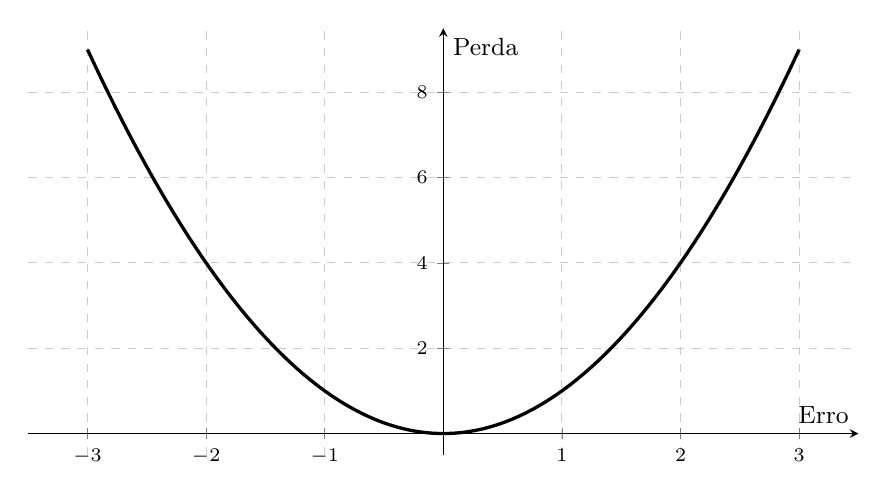
\begin{tikzpicture}
            \begin{axis}[
                width=\linewidth,  
                height=7cm,
                xlabel={Erro},
                ylabel={Perda},
                axis lines=middle,
                grid=major,
                grid style={dashed, gray!40},
                xmin=-3.5, xmax=3.5,
                ymin=-0.5, ymax=9.5,
                legend pos=north west,
                title style={font=\bfseries\small},
                label style={font=\small},
                tick label style={font=\scriptsize}
            ]
                \addplot[
                    domain=-3:3, 
                    samples=100, 
                    color=black, 
                    very thick
                ] {x^2};

            \end{axis}
        \end{tikzpicture}
        \caption{Vista da função de perda em relação ao erro ($\text{Erro} =  y_j - \hat{y}_j$).}%
        \label{fig:mse-2d}
    \end{subfigure}
    \hfill 
    \begin{subfigure}[b]{0.48\textwidth}
        \centering
        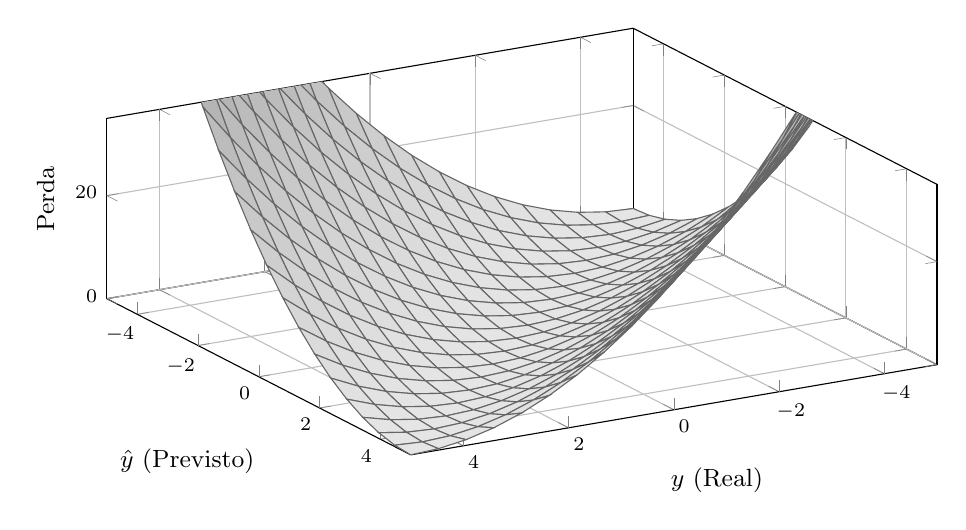
\begin{tikzpicture}
            \begin{axis}[
                width=\linewidth,
                height=7cm,
                xlabel={$y$ (Real)},
                ylabel={$\hat{y}$ (Previsto)},
                zlabel={Perda},
                grid=major,
                view={150}{45}, 
                zmin=0, zmax=35, 
                title style={font=\bfseries\small},
                label style={font=\small},
                tick label style={font=\scriptsize},
                colormap={bw}{gray(0cm)=(0.9); gray(1cm)=(0.5)}
            ]
                \addplot3[
                    surf,           
                    shader=faceted,  
                    faceted color=black!60, 
                    domain=-5:5,    
                    domain y=-5:5,  
                    samples=20,     
                    z buffer=sort
                ] { (x - y)^2 };
            \end{axis}
        \end{tikzpicture}
        \caption{Superfície da função de perda.}%
        \label{fig:mse-3d}
    \end{subfigure}

    \caption{Visualizações do erro quadrático médio em duas e em três dimensões.}%
    \label{fig:mse}
    \fonte{O autor (2025).}
\end{figure}

\subsubsection*{Características do erro quadrático médio}

\begin{description}[style=sameline, leftmargin=1.5em, font=\bfseries\color{black}]
    
    \item[Continuidade e suavidade:] O MSE é uma função de classe $C^{\infty}$, é infinitamente diferenciável (ver Apêndice~\ref{ap:deducoes-mse}). Como consequência, não são encontrados problemas para derivar essa função e também o cálculo do vetor gradiente. Isso torna o MSE uma boa função para ser utilizada em conjunto com otimizadores baseados em gradiente.
    \item[Sensibilidade a \textit{outliers}:] O MSE é uma função que não é Lipschitz-contínua (ver Apêndice~\ref{ap:deducoes-mse}). Caso o erro do modelo treinado cresça exponencialmente, o valor numérico da perda será consideravelmente grande. Não somente isso, ele é sensível a \textit{outliers}, se um grupo de dados fora do padrão estiver presente no conjunto de dados, eles podem enviesar o cálculo da perda, e também na otimização em busca de pontos de mínimo.
    \item[Convexidade:] O MSE é uma função estritamente convexa (ver Apêndice~\ref{ap:deducoes-mse}), representado pelos gráficos da Figura~\ref{fig:mse}, que apresentam uma função com formato de tigela. Dessa forma, essa característica torna-se uma vantagem se estiver sendo utilizados otimizadores baseados em gradiente. Contudo, devido às transformações não-lineares, \textcite{LossesArticle} argumentam que essa propriedade pode deixar de ser verdade em algoritmos de aprendizado profundo.
    \item[Não-negatividade:] omo gráficos da Figura~\ref{fig:mse} ilustram, o MSE é retorna apenas valores positivos. Isso se dá devido à diferença das entradas estar sendo calculada, e, em seguida, elevada ao quadrado, impendido que valores negativos ocorram na saída.
    \item[Baixa interpretabilidade:] O MSE eleva o erro ao quadrado. Ao retornar o valor da perda, não é visto diretamente a distância entre os pontos reais e os pontos preditos pelo modelo. Essa cálculo dificulta saber, de forma rápida, quão bem ou mal o modelo está performando. Funções como a MAE, em que o erro é dado pelo módulo da distância entre os dois pontos são mais diretas em mostrar a performance do modelo;
    
\end{description}

\subsubsection*{Gradiente do erro quadrático médio}

A derivada do erro quadrático médio está na Equação~\ref{eq:mse-derivada}. As derivadas parciais de uma função de perda são de extrema importância para uma rede neural. É partir delas que é calculado o primeiro vetor gradiente, que passa a ser retropropagado por toda a rede no sentido inverso. Indo primeiro das últimas camadas para as camadas de entrada\footnote{Portanto, as derivadas das funções de perda serão discutidas sempre que possível para explicar as características de uma função neste capítulo.}.

\begin{equacaodestaque}{Derivada parcial do erro quadrático médio em relação à predição}
    \frac{\partial\Loss_{\text{MSE}}}{\partial\hat{y}_j} (y_j, \hat{y}_j) = \frac{2}{N} (\hat{y}_j -y_j)%
    \label{eq:mse-derivada}
\end{equacaodestaque}

A Equação~\ref{fig:mse-derivada} mostra a derivada parcial do erro quadrático médio em relação à predição feita pelo modelo $\hat{y}_j$. Mas existe também a derivada parcial em relação ao valor real $y_j$. Juntas, tem-se a Equação~\ref{eq:vetor-gradiente-mse}, que representa o vetor gradiente do MSE. Neste livro será dado um foco maior em apresentar apenas uma das derivadas. Porque, elas muitas vezes apresentarão grandes semelhanças.

\begin{equation}
    \nabla (y_j, \hat{y}_j) = \left( \frac{\partial \Loss_{\text{MSE}}}{\partial y_j}, \frac{\partial \Loss_{\text{MSE}}}{\partial \hat{y}_j} \right)%
    \label{eq:vetor-gradiente-mse}
\end{equation}

Os gráficos da derivada parcial do erro quadrático médio estão ilustrados na Figura~\ref{fig:mse-derivada}. A Figura~\ref{fig:mse-derivada-2d} mostra que o gradiente do MSE é proporcional ao erro do modelo. Um erro alto, gera um gradiente alto, e vice-versa. Quando o modelo está nas primeiras épocas do treinamento, e ainda não se ajustou aos dados, seu erro será alto. Se nesse treinamento estiver sendo utilizado um algoritmo de otimização baseado em gradiente, o ajuste dos parâmetros do modelo será mais brusco. Dado que a variação dos valores dos parâmetros de uma iteração para outra é diretamente proporcional ao vetor gradiente (como explica a Equação~\ref{eq:gradiente-do-erro-em-relacao-a-um-peso-de-um-neuronio-regressao}). Contudo, quando o modelo já tiver melhor se ajustado aos dados, o erro será menor, o gradiente também. Por conseguinte, a retropropagação irá garantir um ajuste fino nos pesos e vieses do modelo.

\begin{figure}[h!]
    \centering 
    \begin{subfigure}[b]{0.48\textwidth}
        \centering
        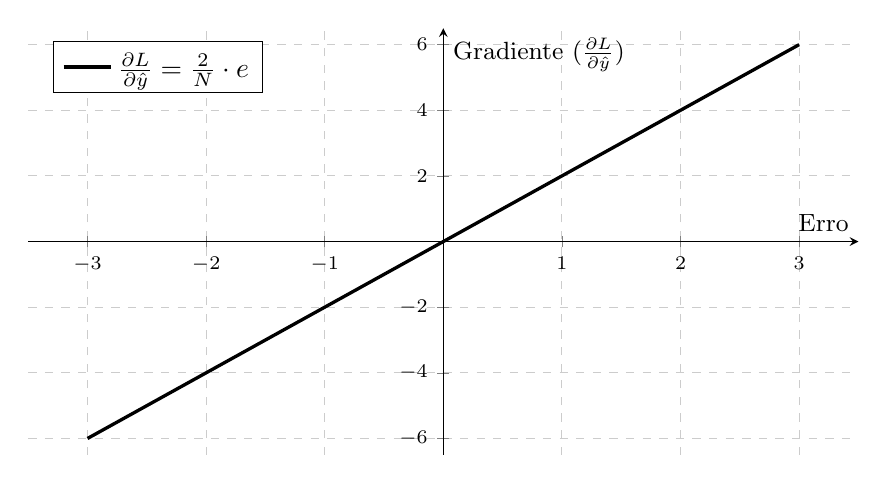
\begin{tikzpicture}
            \begin{axis}[
                width=\linewidth,  
                height=7cm,
                xlabel={Erro},
                ylabel={Gradiente ($\frac{\partial L}{\partial \hat{y}}$)},
                axis lines=middle,
                grid=major,
                grid style={dashed, gray!40},
                xmin=-3.5, xmax=3.5,
                ymin=-6.5, ymax=6.5,
                legend pos=north west,
                title style={font=\bfseries\small},
                label style={font=\small},
                tick label style={font=\scriptsize}
            ]
                \addplot[
                    domain=-3:3, 
                    samples=100, 
                    color=black, 
                    very thick
                ] {2*x};
                \addlegendentry{$\frac{\partial L}{\partial \hat{y}} = \frac{2}{N} \cdot e$}
            \end{axis}
        \end{tikzpicture}
        \caption{Relação linear entre erro e gradiente da perda ($\text{Erro} =  y_j - \hat{y}_j$).}%
        \label{fig:mse-derivada-2d}
    \end{subfigure}
    \hfill 
    \begin{subfigure}[b]{0.48\textwidth}
        \centering
        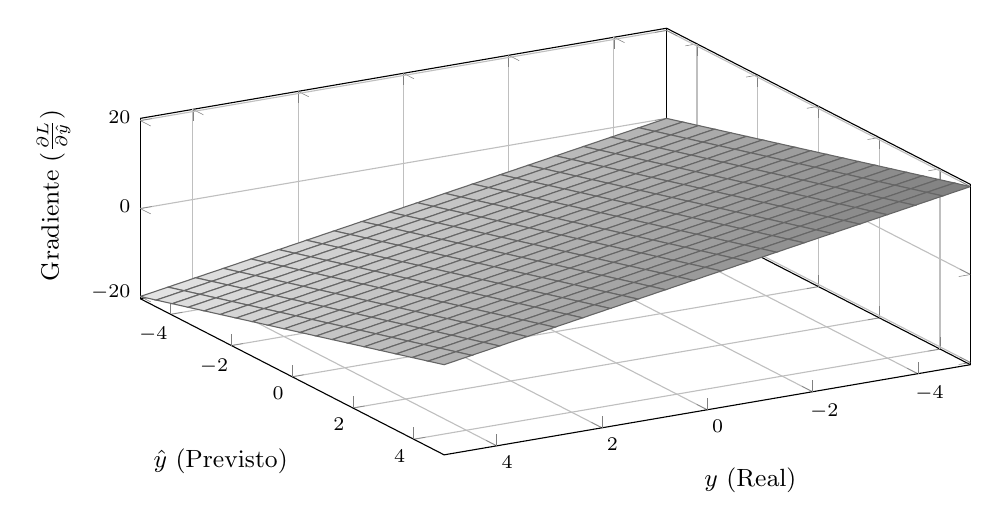
\begin{tikzpicture}
            \begin{axis}[
                width=\linewidth,
                height=7cm,
                xlabel={$y$ (Real)},
                ylabel={$\hat{y}$ (Previsto)},
                zlabel={Gradiente ($\frac{\partial L}{\partial \hat{y}}$)},
                grid=major,
                view={150}{45},
                zmin=-20.5, zmax=20.5,
                title style={font=\bfseries\small},
                label style={font=\small},
                tick label style={font=\scriptsize},
                colormap={bw}{gray(0cm)=(0.9); gray(1cm)=(0.5)}
            ]
                \addplot3[
                    surf,           
                    shader=faceted,  
                    faceted color=black!60, 
                    domain=-5:5,    
                    domain y=-5:5,  
                    samples=20,     
                    z buffer=sort    
                ] { 2 * (y - x) };
            \end{axis}
        \end{tikzpicture}
        \caption{Superfície do gradiente no espaço.}%
        \label{fig:mse-derivada-3d}
    \end{subfigure}

    \caption{Visualizações do gradiente do erro quadrático médio em relação à predição.}%
    \label{fig:mse-derivada}
    \fonte{O autor (2025).}
\end{figure}

\begin{equation}
    \frac{\partial E}{\partial w_{ji}} = \frac{\partial E}{\partial x_j} \cdot y_i \quad \text{ou} \quad \frac{\partial E}{\partial w_{ji}} = \frac{\partial E}{\partial y_j} \cdot \sigma'(x_j) \cdot y_i
    \label{eq:gradiente-do-erro-em-relacao-a-um-peso-de-um-neuronio-perda-regressao}
\end{equation}

\subsubsection*{Raiz do erro quadrático médio (RMSE)}

Além disso, cabe discutir a \textbf{raiz do erro quadrático médio}, também chamada de \textbf{\textit{root mean squared error}} (\textbf{RMSE}). Ela está na Equação~\ref{eq:rmse-metric}. Ela é uma função derivada do MSE, cuja diferença está no cálculo de uma raiz quadrada a partir do resultado do MSE.

\begin{equacaodestaque}{Raiz do erro quadrático médio}
    {RMSE} (y_j, \hat{y}_j) = \sqrt{\frac{1}{N} \sum_{j=1}^{N} (y_j -\hat{y}_j)^2}%
    \label{eq:rmse-metric}
\end{equacaodestaque}

A RMSE serve de métrica para avaliar os modelos de regressão. O MSE funciona como uma função de perda bem como uma métrica avaliativa. Mas, é difícil interpretar a primeira vista os seus resultados, uma vez que ele eleva ao quadrado o cálculo do erro. Com a RMSE é resolvido esse ``problema'' da interpretabilidade, gerando um resultado mais tangível para entender como o modelo está performando.

\subsubsection*{Aplicações do erro quadrático médio}%
\index{Aplicações práticas! Erro quadrático médio (MSE)}

\begin{description}[style=sameline, leftmargin=1.5em, font=\bfseries\color{black}] 
    \item[Estimação de custos médicos (saúde):] Para fazer previsões de custos médicos \textcite{MedicalCostsEstimationUsingLR} utilizam técnicas de regressão, para avaliar os modelos criados, os autores utilizam o MSE, MAE e $R^2$ como métricas.
    \item[Estimação de preços de imóveis (mercado imobiliário):] \textcite{OptimalHousePricePrediction} criam modelos de regressão (como regressão linear, florestas aleatórias e XGBoost) com intuito de prever valores de casas, eles fazem uso do MSE e da RMSE para avaliar o desempenho.
    \item[Previsão da produção agrícola (agronomia):] \textcite{CouplingMachineLearningAndCropModeling} combinam aprendizado de máquina com modelagem de culturas para prever a produção das plantações na região do cinturão do milho nos Estados Unidos. Para avaliar as predições, eles utilizam a RMSE como métrica \parencite{CouplingMachineLearningAndCropModeling}
    \item[Previsão de demanda de energia (gestão energética):] \textcite{OptimizingFL} fazem uma adaptação do MSE transformando-o no \textit{Exponentially Weighted Mean Squared Error} (\textit{EW-RSM}), essa adaptação é justificada como uma forma de enfatizar a acurácia em previsões de longo prazo atribuindo pesos exponencialmente crescentes aos erros em etapas de tempo posteriores.
\end{description}

\medskip

O erro quadrático médio é ideal para ser utilizado em cenários que deve-se garantir uma maior penalização dos erros do modelo que durante seu treinamento. Isso acontece devido à sua sensibilidade a \textit{outliers}. Entretanto, vão existir cenários em que essa propriedade pode ser uma desvantagem, enviesando o treinamento de um modelo de regressão. Diante disso, alternativas como o erro absoluto médio tornam-se mais viáveis.

\subsection{Erro absoluto médio (MAE)}%
\index{Funções de Perda!Erro absoluto médio (MAE)}%
\label{sec:mae-loss}

O \textbf{erro absoluto médio}, também chamado de \textbf{perda L1}, é uma função que tem o mesmo propósito do erro quadrático médio, ser utilizada em tarefas de regressão. Ele não possui uma origem definida como o MSE, esse conceito de minimizar a diferença de um resultado pelo seu valor real já havia sendo utilizado há bastante tempo. 

Trabalhos como \textit{Greedy function approximation: A gradient boosting machine} de \textcite{GreedyFunctionApproximation} utilizam essa função de perda para resolver problemas de aprendizado de máquina. No texto, o autor desenvolve um algoritmo de \textit{boosting} específico para o MAE (o qual é apresentado com outro nome, \textbf{\textit{Least-Absolute-Deviation}} (\textbf{LAD})), sendo responsável por dar nome ao algoritmo criado, o \texttt{LAD\_TreeBoost} \parencite{GreedyFunctionApproximation}. \textcite{GreedyFunctionApproximation} explica que esse algoritmo utiliza uma árvore de regressão com a perda, para prever a pseudo-resposta que é o sinal dos resíduos atuais. Como consequência, o modelo é atualizado adicionando em cada nó terminal da nova árvore criada a mediana dos resíduos daquela região específica.

Um trabalho mais recente que explora o uso dessa função é o \textit{Image-to-Image Translation with Conditional Adversarial Networks} \parencite{ImageToImage}. Nele, \textcite{ImageToImage} argumentam que preferiram trabalhar com a distância L1 (um dos diferentes nomes utilizados para se referir ao MAE) devido à ela gerar imagens menos borradas. A comparação das funções de perda utilizadas na pesquisa está nas imagens da Figura~\ref{fig:comparativo-perdas-image-to-image}. A perda que apresenta os resultados mais consistentes com a realidade é a L1 + cGAN, a qual possuí o MAE em sua composição.

\begin{figure}[h]
    \centering
    \includegraphics[width=0.65\linewidth]{../imagens/perda-regressao/image-to-image-perdas-comparativo.png}
    
    \caption[Perdas diferentes induzem qualidades de resultados diferentes. Cada coluna mostra resultados treinados sob uma perda diferente de aprendizado no dataset MNIST]{%
        Perdas diferentes induzem qualidades de resultados diferentes. Cada coluna mostra resultados treinados sob uma perda diferente de aprendizado no dataset MNIST
        \newline
        \small Fonte: \parencite{ImageToImage}.
    }%
    \label{fig:comparativo-perdas-image-to-image}
\end{figure}

Voltando para a analogia dos dardos. Consideramos que será feito um novo jogo com dez participantes, no jogo, cada um tem direito de jogar apenas um dardo. No final, os dardos serão somados e será dado o resultado da equipe. Se tivéssemos uma equipe muito ruim utilizando como métrica o MSE para avaliar os pontos, o resultado seria péssimo. Os dardos estariam muito longes do centro, e, como o erro é elevado ao quadrado, isso geraria uma pontuação ainda menor. 

Contudo, se a métrica escolhida para avaliar o jogo fosse o MAE o resultado seria melhor. Visto que, o erro cresce de forma linear. No contexto de aprendizado de máquina, os jogadores ruins se comparam com os \textit{outliers}, eles estão presentes nos dados e vão enviesar o aprendizado do modelo. Entretanto, utilizar uma função que não seja tão sensível na medição desses valores extremos pode ser uma boa alternativa para cenários em que essa configuração será comum.

O MAE está definido na Equação~\ref{eq:mae}. Essa função de perda avalia a diferença entre dois pontos: o valor real $y_j$ e o valor predito $\hat{y}_j$, para todos os $N$ casos analisados. A partir disso, calcula a média dos resultados, retornando o valor final para a perda do modelo.

\begin{equacaodestaque}{Erro absoluto médio}
    \Loss_{\text{MAE}} (y_j, \hat{y}_j) = \frac{1}{N} \sum_{j=1}^{N} |y_j -\hat{y}_j|%
    \label{eq:mae}
\end{equacaodestaque}

Em que:

\begin{description}[style=sameline, leftmargin=1.5em, font=\bfseries\color{black}]  
    \item[$y_j$] representa o valor real da j-ésima amostra;
    \item[ $\hat{y}_j$] representa o valor predito pelo modelo para a j-ésima amostra;
    \item[$N$] representa o número de amostras.
\end{description}

 Diferente do erro quadrático médio, o MAE cresce de forma linear, como é mostrado na Figura~\ref{fig:mae}. Isso garante para essa função de perda uma melhor capacidade de lidar com \textit{outliers}, dado que o erro não irá aumentar de forma exacerbada como acontecia no MSE. O MAE também apresenta uma ``quina'', nos pontos em que o cálculo do erro é nulo. Dessa forma, essa função não pode ser classificada como suave em todo o seu domínio.

\begin{figure}[h!]
    \centering
    \begin{subfigure}[b]{0.48\textwidth}
        \centering
        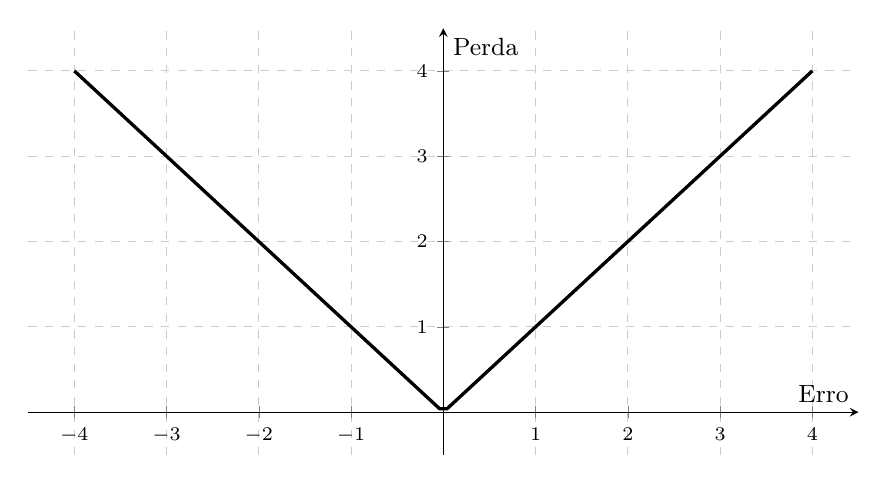
\begin{tikzpicture}
            \begin{axis}[
                width=\linewidth,  
                height=7cm,
                xlabel={Erro},
                ylabel={Perda},
                axis lines=middle,
                grid=major,
                grid style={dashed, gray!40},
                xmin=-4.5, xmax=4.5,
                ymin=-0.5, ymax=4.5,
                legend pos=north west,
                title style={font=\bfseries\small},
                label style={font=\small},
                tick label style={font=\scriptsize}
            ]
                \addplot[
                    domain=-4:4, 
                    samples=100, 
                    color=black, 
                    very thick
                ] {abs(x)};
            \end{axis}
        \end{tikzpicture}
        \caption{Vista da função de perda em relação ao erro ($\text{Erro} =  y_j - \hat{y}_j$).}%
        \label{fig:mae-2d}
    \end{subfigure}
    \hfill
    \begin{subfigure}[b]{0.48\textwidth}
        \centering
        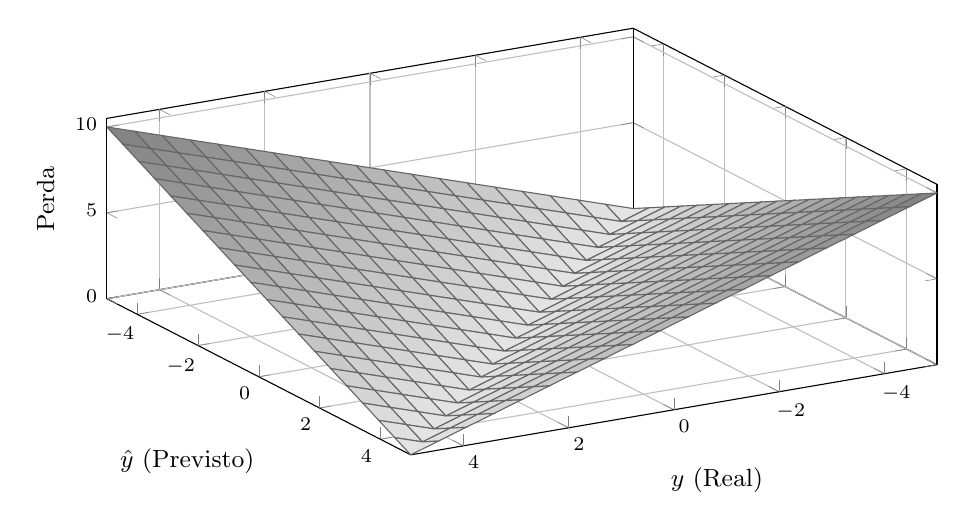
\begin{tikzpicture}
            \begin{axis}[
                width=\linewidth,
                height=7cm,
                xlabel={$y$ (Real)},
                ylabel={$\hat{y}$ (Previsto)},
                zlabel={Perda},
                grid=major,
                view={150}{45}, 
                zmin=0, zmax=10.5, 
                title style={font=\bfseries\small},
                label style={font=\small},
                tick label style={font=\scriptsize},
                colormap={bw}{gray(0cm)=(0.9); gray(1cm)=(0.5)}
            ]
                \addplot3[     
                    surf,         
                    shader=faceted,  
                    faceted color=black!60, 
                    domain=-5:5,    
                    domain y=-5:5,  
                    samples=20,     
                    z buffer=sort  
                ] { abs(x - y) };
            \end{axis}
        \end{tikzpicture}
        \caption{Superfície da função de perda.}%
        \label{fig:mae-3d}
    \end{subfigure}

    \caption{Visualizações da função de perda erro absoluto médio em duas e em três dimensões.}%
    \label{fig:mae}
    \fonte{O autor (2025).}
\end{figure}

\subsubsection*{Características do erro absoluto médio}

\begin{description}[style=sameline, leftmargin=1.5em, font=\bfseries\color{black}] 
    \item[Continuidade, suavidade e diferenciabilidade:] O MAE é uma função de classe $C^0$ (ver Apêndice~\ref{ap:deducoes-mae}). Ele é contínuo em todo o seu domínio, mas, devido ao ``bico'' quando o erro é zero, não pode ser totalmente derivado. Essa característica não impede que o erro absoluto médio seja utilizado em conjunto com otimizadores baseados em gradiente. Como será visto, é possível contornar esse problema com o cálculo do subgradiente.
    \item[Convexidade:] O MAE é convexo (ver Apêndice~\ref{ap:deducoes-mae}). Como o teorema de \textbf{Convexidade de Normas e Máximos} afirma, toda função modular é convexa como consequência da desigualdade triangular. Isso também está explicitado nos gráficos da Figura~\ref{fig:mae}, com o formato em ``V'' da função de perda.
    \item[Robustez para \textit{outliers}:] Como é apontado na Figura~\ref{fig:mae}, o erro absoluto médio não retorna valores negativos para nenhum valor de entrada. A sua saída saída será sempre positiva ou zero, independente da entrada. Isso se dá, devido à propriedade do módulo, que não admite números negativos para sua saída;
    \item[Não-derivável em zero:] Esse ponto acontece devido à forma que a função módulo é representa graficamente, ela tem a forma de um ``bico'' em zero. Para contornar esse problema, pode ser utilizado o subgradiente.
    \item[Boa interpretabilidade:] Diferente do erro quadrático médio em que o erro total é elevado ao quadrado, no MAE isso não ocorre. O erro é simplesmente a média das diferenças dos pontos. É intuitivo interpretar os resultados que essa função de perda retorna, considerando que não é preciso fazer nenhum cálculo adicional para ter uma noção precisa se as previsões feitas pelo modelo condizentes ou não dos valores reais.
\end{description}

\subsubsection*{Gradiente do erro absoluto médio}

Como destacado anteriormente, o MAE não é diferenciável em zero. Assim, pode-se ter a ideia de que devido a isso, essa não seja uma boa função para ser utilizada em conjunto com otimizadores baseados em gradiente. Contudo, existe uma forma de contornar esse problema da não-diferenciabilidade: o subgradiente.

O subgradiente é uma estratégia que generaliza a derivada para funções convexas não-diferenciáveis, um exemplo disso é a função módulo de $x$. Em vez de um único valor em um determinado ponto, o subgradiente retorna um conjunto de valores possíveis para a inclinação da reta tangente.
 
Matematicamente, a derivada da função módulo com o subgradiente é dada por:

\begin{enumerate}
    \item Para $x > 0$: A função comporta-se como $f(x) = x$. A derivada é $1$;
    \item Para $x < 0$: A função comporta-se como $f(x) = -x$. A derivada é $-1$;
    \item Para $x = 0$: O subgradiente é o intervalo de todas as inclinações possíveis entre $-1$ e $1$.
\end{enumerate}

Ao utilizar o subgradiente para calcular a derivada parcial do erro absoluto médio em relação à predição $\hat{y}_j$ é encontrada a Equação~\ref{eq:mae-derivada}.

\begin{equacaodestaque}{Derivada parcial do erro absoluto médio em Relação à predição}
    \frac{\partial\Loss_{\text{MAE}}}{\partial\hat{y}_j} (y_j, \hat{y}_j) = 
    \begin{cases} 
      -1 & \text{se } \hat{y}_j > y_j \\
      +1 & \text{se } \hat{y}_j < y_j \\
      [-1, +1] & \text{se } \hat{y}_j = y_j
    \end{cases}%
    \label{eq:mae-derivada}
\end{equacaodestaque}

 Pelo fato do MAE ser uma função que não é diferenciável em todos o seu domínio, isso reflete no jeito com que o gráficos da derivada são representados, os quais estão na Figura~\ref{fig:mae-derivada}. Existem, também na derivada, pontos de descontinuidade, fazendo com que o gráfico dessa função se assemelhe ao gráfico da função de ativação degrau unitário. Esses pontos de descontinuidade, estão exatamente em zero, assim como na função original.

Diferente do MSE que é uma parábola, e portanto, ao ser derivado, gera o gráfico de uma reta que cresce de forma linear. O MAE gera o gráfico de duas retas constantes, dado que a derivada de uma função linear é uma função constante.

\begin{figure}[h!]
    \centering
    \begin{subfigure}[b]{0.48\textwidth}
        \centering
        \begin{tikzpicture}
            \begin{axis}[
                width=\linewidth,  
                height=7cm,
                xlabel={Erro},
                ylabel={Gradiente ($\frac{\partial L}{\partial \hat{y}}$)},
                axis lines=middle,
                grid=major,
                grid style={dashed, gray!40},
                xmin=-3.5, xmax=3.5,      
                ymin=-1.5, ymax=1.5,   
                ytick={-1, 0, 1},     
                legend pos=north west,
                title style={font=\bfseries\small},
                label style={font=\small},
                tick label style={font=\scriptsize}
            ]
                \addplot[
                    domain=-3:0, 
                    samples=100, 
                    color=black, 
                    very thick
                ] {-1};
                \addplot[
                    domain=0:3, 
                    samples=100, 
                    color=black, 
                    very thick
                ] {1};
                \addplot[only marks, mark=o, color=black, mark size=2pt] coordinates {(0,-1) (0,1)};
            \end{axis}
        \end{tikzpicture}
        \caption{Relação constante por partes entre erro e gradiente da perda ($\text{Erro} =  y_j - \hat{y}_j$).}%
        \label{fig:mae-derivada-2d}
    \end{subfigure}
    \hfill 
    \begin{subfigure}[b]{0.48\textwidth}
        \centering
        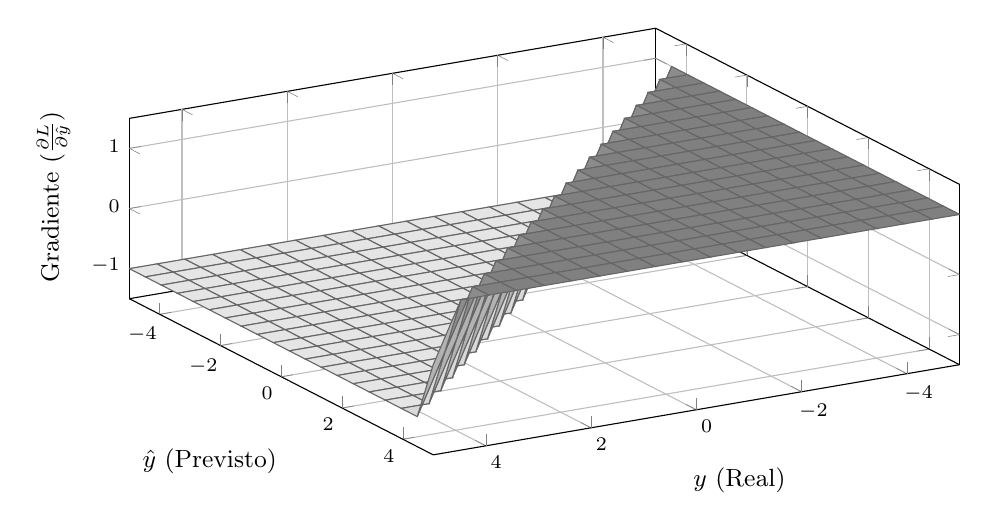
\begin{tikzpicture}
            \begin{axis}[
                width=\linewidth,
                height=7cm,
                xlabel={$y$ (Real)},
                ylabel={$\hat{y}$ (Previsto)},
                zlabel={Gradiente ($\frac{\partial L}{\partial \hat{y}}$)},
                grid=major,
                view={150}{45},
                zmin=-1.5, zmax=1.5, 
                ztick={-1, 0, 1},
                title style={font=\bfseries\small},
                label style={font=\small},
                tick label style={font=\scriptsize},
                colormap={bw}{gray(0cm)=(0.9); gray(1cm)=(0.5)}
            ]
                \addplot3[ 
                    surf,           
                    shader=faceted,  
                    faceted color=black!60, 
                    domain=-5:5,    
                    domain y=-5:5,  
                    samples=20,     
                    z buffer=sort
                ] { sign(y - x) };
            \end{axis}
        \end{tikzpicture}
        \caption{Superfície do gradiente no espaço.}%
        \label{fig:mae-derivada-3d}
    \end{subfigure}

    \caption{Visualizações do gradiente do erro absoluto médio em relação à predição.}%
    \label{fig:mae-derivada}
    \fonte{O autor (2025).}
\end{figure}

\subsubsection*{Aplicações do erro absoluto médio}%
\index{Aplicações práticas! Erro absoluto médio (MAE)}

\begin{description}[style=sameline, leftmargin=1.5em, font=\bfseries\color{black}] 
    \item[Avaliação de idade óssea e estimação do escore de cálcio na artéria coronária (Saúde):] \textcite{chao2022regressionmetriclosslearning} desenvolvem algoritmos de regressão para estimar escore de cálcio da artéria coronária além de um segundo algoritmo para avaliação da idade óssea. Como forma de avaliar as previsões \textcite{chao2022regressionmetriclosslearning} utilizam o MAE em uma das métricas.
    \item[Restauração de imagens (Engenharia):] \textcite{Noise2Noise} estavam buscando uma maneira ideal de remover textos de imagens, de forma que o MAE, por ser uma função de perda robusta, conseguiu atingir bons resultados nessa tarefa.
    \item[Previsão da produção de energia eólica (Setor energético):] \textcite{MinimumOpenDataSubsetForWindPowerPrediction} utilizam um modelo de florestas aleatórias para prever a produção de energia eólica. Os autores avaliam o desempenho com as funções MAE  e RMSE \parencite{MinimumOpenDataSubsetForWindPowerPrediction}.
    \item[Previsão de poluição do ar (Setor ambiental):] \textcite{nedungadi2025aircastimprovingairpollution} buscam formas de melhorar a previsão da poluição do ar, os pesquisadores utilizam uma função inspirada pelo MAE, o \textit{Frequency-weighted Mean Absolute Error} (\textit{fMAE}), tendo como principal vantagem lidar com variáveis que apresentam uma distribuição de cauda pesada.
\end{description}

\medskip

O erro quadrático médio penaliza em maior grau os \textit{outliers}, enquanto o erro absoluto médio é uma função robusta a \textit{outliers}. Contudo, pode ser necessário ter uma função que combine essas duas características. De forma que ela penalize em maior força os erros pequenos, mas ao mesmo tempo seja robusta a \textit{outliers}, permitindo evitar que o modelo seja enviesado no treinamento. Nesses casos, uma solução é a perda de Huber.

\subsection{Perda de Huber (Huber loss)}%
\index{Funções de Perda!Perda de Huber (Huber loss)}%
\label{sec:huber-loss}

Proposta por Peter J. Huber, a \textbf{perda de Huber}, também chamada de \textit{\textbf{Huber loss}} foi apresentada no trabalho \textit{Robust Estimation of a Location Parameter} \parencite{HuberLoss}. \textcite{HuberLoss} estudava maneiras de fazer uma estimação robusta de um parâmetro de localização (como a média o mediana de um conjunto de dados) quando a distribuição dos dados é aproximadamente conhecida. Para solucionar esse problema, o autor define um estimador robusto $p$ que segue a Equação~\ref{eq:huber-loss-do-huber} \parencite{HuberLoss}.

\begin{equation}
    \rho(t) = 
    \begin{cases}
        \frac{1}{2} t^2 & \text{se} |t| < k \\
        k |t| - \frac{1}{2} k^2 & \text{se} t \ge k
    \end{cases}
    \label{eq:huber-loss-do-huber}
\end{equation}

Ao desenvolver a Equação~\ref{eq:huber-loss-do-huber}, Huber cria uma função que comportava de forma quadrática, semelhante ao MSE para os casos em que $|t| < k$. Já para os casos em que $t \ge k$, a função cresce linearmente, como o MAE. Essa função criada pelo pesquisador é a perda de Huber, que, representada com as notações deste livro, está na Equação~\ref{eq:huber-loss}.

\begin{equacaodestaque}{Perda de Huber}
    \Loss_{\text{Huber}} (y, \hat{y}) = 
    \begin{cases} 
      \frac{1}{2} (y -\hat{y})^2 & \text{para } |y -\hat{y}| \le\delta\\
      \delta(|y -\hat{y}| -\frac{1}{2}\delta) & \text{caso contrário}
    \end{cases}%
    \label{eq:huber-loss}
\end{equacaodestaque}

Em que:

\begin{description}[style=sameline, leftmargin=1.5em, font=\bfseries\color{black}]  
    \item[$y_j$] representa o valor real da j-ésima amostra;
    \item[ $\hat{y}_j$] representa o valor predito pelo modelo para a j-ésima amostra;
    \item[$N$] representa o número de amostras;
    \item[$\delta$] representa o parâmetro de sensibilidade. 
\end{description}

Como a Figura~\ref{fig:huber-loss} evidencia, a perda de Huber é uma função ``híbrida'', apresentando dois comportamentos distintos. Até o valor em que o erro é menor que o parâmetro $\delta$, a perda segue o formato de uma parábola. Quando o erro torna-se maior que $\delta$, a perda passa a ser linear. Pode-se pensar que nessas junções, em que o erro é igual a $\delta$, seriam formados ``bicos'' afetando a suavidade da função. Contudo, a perda de Huber é uma função de classe $\mathbb{C}^1$, o que significa que ela é suave, contínua e diferenciável em todo o seu domínio para a primeira derivada. Isso pode ser um problema para aqueles otimizadores que são de segunda ordem, como o método de Newton-Raphson, neste caso, eles dependem que a função seja de classe $\mathbb{C}^2$ para conseguir encontrar pontos de mínimo.

\begin{figure}[h!]
    \centering
    \begin{subfigure}[b]{0.48\textwidth}
        \centering
        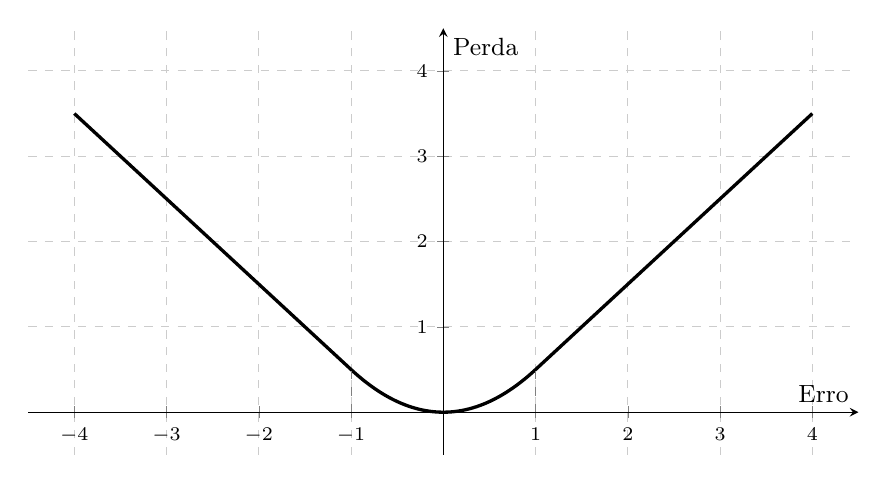
\begin{tikzpicture}
            \def\delta{1.0} 
            
            \begin{axis}[
                width=\linewidth,  
                height=7cm,
                xlabel={Erro},
                ylabel={Perda},
                axis lines=middle,
                grid=major,
                grid style={dashed, gray!40},
                xmin=-4.5, xmax=4.5,  
                ymin=-0.5, ymax=4.5,      
                legend pos=north west,
                title style={font=\bfseries\small},
                label style={font=\small},
                tick label style={font=\scriptsize}
            ]
                \addplot[
                    domain=-4:4, 
                    samples=201, 
                    color=black, 
                    very thick
                ] { abs(x) <= \delta ? 0.5*x^2 : \delta*(abs(x) - 0.5*\delta) };

                \draw[dashed, gray] (axis cs:-\delta, 0) -- (axis cs:-\delta, {\delta*(\delta-0.5*\delta)});
                \draw[dashed, gray] (axis cs:\delta, 0) -- (axis cs:\delta, {\delta*(\delta-0.5*\delta)});
            \end{axis}
        \end{tikzpicture}
        \caption{Vista da função de perda em relação ao erro ($\text{Erro} =  y_j - \hat{y}_j$).}%
        \label{fig:huber-2d}
    \end{subfigure}
    \hfill 
    \begin{subfigure}[b]{0.48\textwidth}
        \centering
        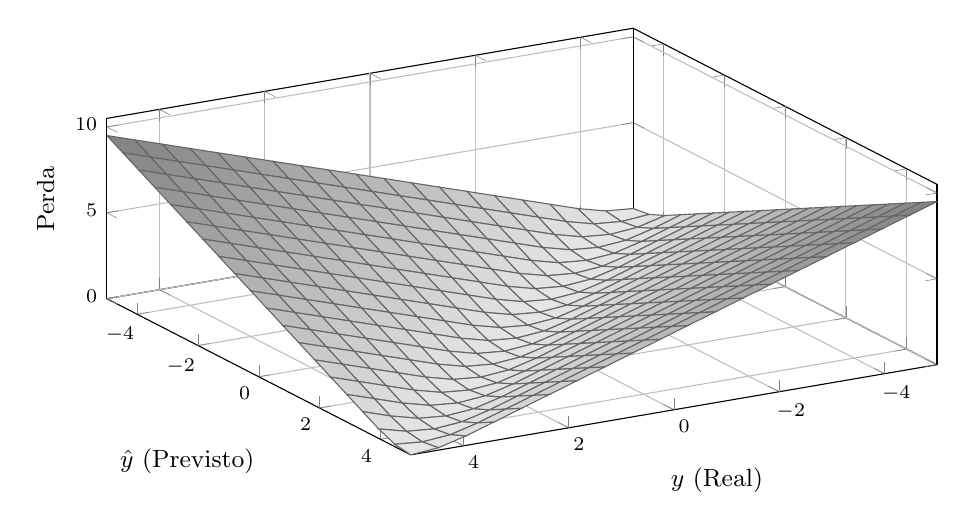
\begin{tikzpicture}

            \def\delta{1.0}
            
            \begin{axis}[
                width=\linewidth,
                height=7cm,
                xlabel={$y$ (Real)},
                ylabel={$\hat{y}$ (Previsto)},
                zlabel={Perda},
                grid=major,
                view={150}{45},
                zmin=0, zmax=10.5,
                title style={font=\bfseries\small},
                label style={font=\small},
                tick label style={font=\scriptsize},
                colormap={bw}{gray(0cm)=(0.9); gray(1cm)=(0.5)}
            ]
                \addplot3[
                    surf,           
                    shader=faceted,  
                    faceted color=black!60, 
                    domain=-5:5,    
                    domain y=-5:5,  
                    samples=20,     
                    z buffer=sort
                ] { abs(x-y) <= \delta ? 0.5*(x-y)^2 : \delta*(abs(x-y) - 0.5*\delta) };
            \end{axis}
        \end{tikzpicture}
        \caption{Superfície da função de perda.}%
        \label{fig:huber-3d}
    \end{subfigure}

    \caption{Visualizações da função de perda de Huber (com $\delta=1$) em duas e em três dimensões.}%
    \label{fig:huber-loss}
    \fonte{O autor (2025).}
\end{figure}

O hiperparâmetro $\delta$ serve para ajustar a sensibilidade da perda de Huber. Um valor muito alto, demonstrado na Figura~\ref{fig:huber-2d-d40}, torna a função muito sensível ao erro e também a \textit{outliers}. Ela também se assemelha com os gráficos do erro quadrático médio, dado que para grande parte de seu domínio, ela calcula o erro de forma quadrática. Um valor muito pequeno para $\delta$, como na Figura~\ref{fig:huber-2d-d05}, faz com que a parábola da perda de Huber seja curta. Com isso, a função apresenta uma melhor robustez a \textit{outliers}, se assemelhando com o erro absoluto médio.

\begin{figure}[h!]
    \centering
    \begin{subfigure}[b]{0.48\textwidth}
        \centering
        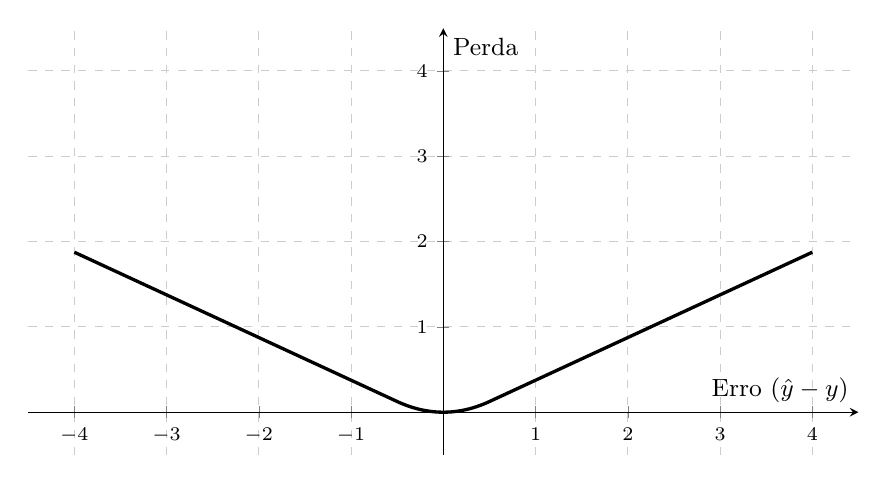
\begin{tikzpicture}
            \def\delta{0.5} 
            \begin{axis}[
                width=\linewidth,
                height=7cm,
                xlabel={Erro ($\hat{y} - y$)},
                ylabel={Perda},
                axis lines=middle,
                grid=major,
                grid style={dashed, gray!40},
                xmin=-4.5, xmax=4.5,
                ymin=-0.5, ymax=4.5,
                legend pos=north west,
                title style={font=\bfseries\small},
                label style={font=\small},
                tick label style={font=\scriptsize},
            ]
                \addplot[
                    domain=-4:4, 
                    samples=201, 
                    color=black, 
                    very thick,
                ] {(abs(x) <= \delta) ? (0.5*x^2) : (\delta*(abs(x) - 0.5*\delta))};
            \end{axis}
        \end{tikzpicture}
        \caption{Perda 2D com $\delta = 0.5$.}
        \label{fig:huber-2d-d05}
    \end{subfigure}
    \hfill
    \begin{subfigure}[b]{0.48\textwidth}
        \centering
        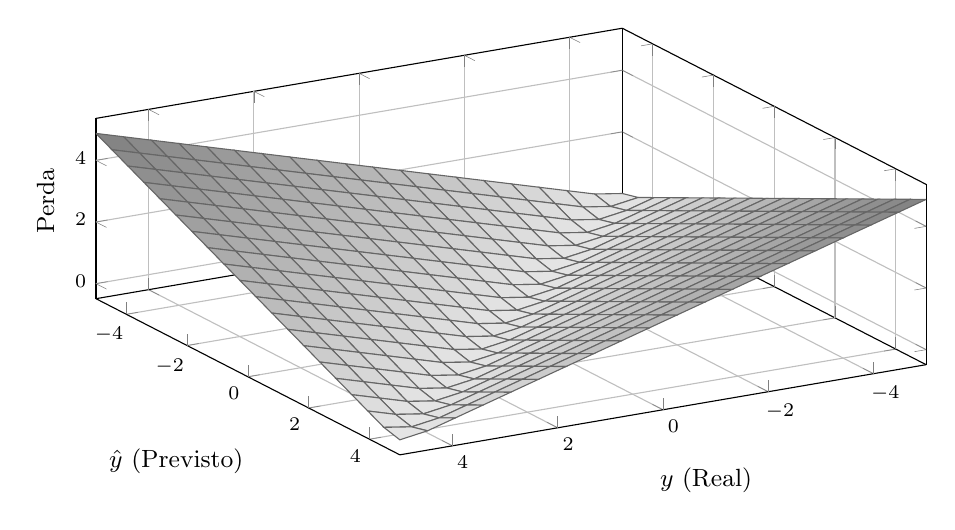
\begin{tikzpicture}
             \def\delta{0.5}
            \begin{axis}[
                width=\linewidth,
                height=7cm,
                xlabel={$y$ (Real)},
                ylabel={$\hat{y}$ (Previsto)},
                zlabel={Perda},
                grid=major,
                view={150}{45},
                legend pos=north east,
                title style={font=\bfseries\small},
                label style={font=\small},
                tick label style={font=\scriptsize},
                colormap={bw}{gray(0cm)=(0.9); gray(1cm)=(0.5)}
            ]
                \addplot3[
                    surf,           
                    shader=faceted,  
                    faceted color=black!60, 
                    domain=-5:5,    
                    domain y=-5:5,  
                    samples=20,     
                    z buffer=sort 
                ] 
                { (abs(y-x) <= \delta) ? (0.5*(y-x)^2) : (\delta*(abs(y-x) - 0.5*\delta)) };
            \end{axis}
        \end{tikzpicture}
        \caption{Superfície com $\delta = 0.5$.}
        \label{fig:huber-3d-d05}
    \end{subfigure}

    \vspace{0.5cm} 

    \begin{subfigure}[b]{0.48\textwidth}
        \centering
        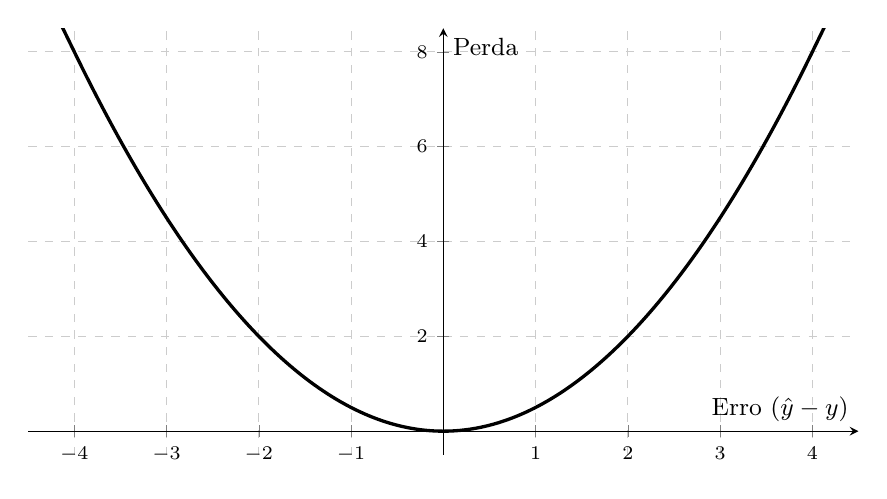
\begin{tikzpicture}
            \def\delta{4.0}
            \begin{axis}[
                width=\linewidth,
                height=7cm,
                xlabel={Erro ($\hat{y} - y$)},
                ylabel={Perda},
                axis lines=middle,
                grid=major,
                grid style={dashed, gray!40},
                xmin=-4.5, xmax=4.5,
                ymin=-0.5, ymax=8.5,
                legend pos=north west,
                title style={font=\bfseries\small},
                label style={font=\small},
                tick label style={font=\scriptsize},
            ]
                \addplot[
                    domain=-4.5:4.5, 
                    samples=201, 
                    color=black, 
                    very thick
                ] {(abs(x) <= \delta) ? (0.5*x^2) : (\delta*(abs(x) - 0.5*\delta))};
            \end{axis}
        \end{tikzpicture}
        \caption{Perda com $\delta = 4.0$.}
        \label{fig:huber-2d-d40}
    \end{subfigure}
    \hfill
    \begin{subfigure}[b]{0.48\textwidth}
        \centering
        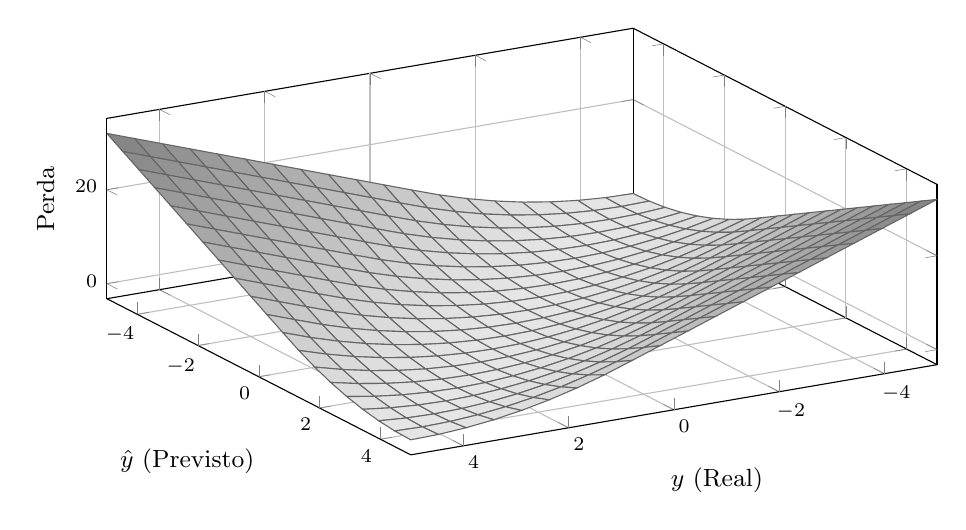
\begin{tikzpicture}
            \def\delta{4.0} 
            \begin{axis}[
                width=\linewidth,
                height=7cm,
                xlabel={$y$ (Real)},
                ylabel={$\hat{y}$ (Previsto)},
                zlabel={Perda},
                grid=major,
                view={150}{45},
                legend pos=north east,
                title style={font=\bfseries\small},
                label style={font=\small},
                tick label style={font=\scriptsize},
                colormap={bw}{gray(0cm)=(0.9); gray(1cm)=(0.5)}
            ]
                \addplot3[
                    surf,           
                    shader=faceted,  
                    faceted color=black!60, 
                    domain=-5:5,    
                    domain y=-5:5,  
                    samples=20,     
                    z buffer=sort    
                ] 
                { (abs(y-x) <= \delta) ? (0.5*(y-x)^2) : (\delta*(abs(y-x) - 0.5*\delta)) };
            \end{axis}
        \end{tikzpicture}
        \caption{Superfície com $\delta = 4.0$.}
        \label{fig:huber-3d-d40}
    \end{subfigure}
    
    \caption{Visualização da Perda de Huber em duas e três dimensões variando o hiperparâmetro $\delta$.}%
    \label{fig:huber-grid-comparacao}
    \fonte{O autor (2025).}
\end{figure}

\subsubsection*{Características da perda de Huber}

\begin{description}[style=sameline, leftmargin=1.5em, font=\bfseries\color{black}] 
    \item[Continuidade, suavidade e diferenciabilidade:] Como dito anteriormente a perda de Huber é uma função de classe $C^1$ (ver Apêndice~\ref{ap:deducoes-huber-loss}). Isso implica em facilidades para encontrar as derivadas parciais e o vetor gradiente dessa função de perda.
    \item[Convexidade:] A perda de Huber é uma função convexa (ver Apêndice~\ref{ap:deducoes-huber-loss}). Ela apresenta o formato característico de um funil. Como resultado, é esperado que a busca por pontos de mínimo utilizando métodos baseados em gradiente seja feita sem muitos problemas de convergência dependendo do tamanho do passo escolhido. Assim como as outras funções, essa convexidade pode ser alterada caso seja utilizada em modelos de aprendizado profundo.
    \item[Robustez para \textit{outliers}:] A perda de Huber é uma função Lipschitz-contínua (ver Apêndice~\ref{ap:deducoes-huber-loss}). Assim como o erro absoluto médio, o maior valor que a derivada da perda de Huber pode alcançar é 1, não existindo risco de ocorrer explosões do gradiente ao calcular o valor inicial da perda.
    \item[Hiperparâmetro $\delta$:] A perda de Huber adiciona um novo hiperparâmetro para a construção de um modelo de aprendizado. Ela dá a possibilidade de que seja controlado como os erros são calculados, contudo, $\delta$ não é ajustado automaticamente como os pesos e vieses na retropropagação. Um novo hiperparâmetro, significa ainda mais testes para encontrar seu valor ideal, isso costuma levar tempo, o que pode não ser ideal em certos casos.
\end{description}

\subsubsection*{Gradiente da perda de Huber}

Dado que a perda de Huber é uma função por partes, a suas derivadas devem levar isso em consideração. Para os casos em que $|y - \hat{y}|  \le \delta$, a função que antes comportava de forma quadrática, ao ser derivada, torna-se uma reta afim. Já em $|y - \hat{y}|$, o comportamento linear, vira uma reta constante. Nessa situação, a função depende da derivada da função módulo, que é dado pelo termo $\text{sgn}$. 

A derivada da parcial da perda de Huber em relação à predição é dada pela Equação~\ref{eq:huber-loss-derivada}.

\begin{equacaodestaque}{Derivada parcial da perda de Huber em relação à predição}
    \frac{\partial\Loss_{\delta}}{\partial\hat{y}} (y_j, \hat{y}_j) = 
    \begin{cases} 
        \hat{y} -y & \text{se } | y -\hat{y} | \le\delta\\
        \delta\cdot \text{sgn} (\hat{y} -y) & \text{se } | y -\hat{y} | > \delta\end{cases}%
    \label{eq:huber-loss-derivada}
\end{equacaodestaque}

Uma vantagem da derivada da perda de Huber é que ela permite naturalmente um \textit{gradient clipping} para evitar que o gradiente exploda. Isso acontece, porque a parte que antes era linear, na derivada é constante. O que significa, que independentemente do valor de entrada, se ele for maior que $\delta$, ele não irá crescer. Ele será dado por $\delta \text{sgn} (\hat{y} - y)$, que é uma reta constante.

O comportamento híbrido da perda de Huber está presente em sua derivada, como é apontado na Figura~\ref{eq:huber-loss-derivada}. A derivada da perda de Huber deixa de ser suave, sendo composta de quatro retas, duas afim, e duas retas constantes. 

\begin{figure}[h!]
    \centering 

    \begin{subfigure}[b]{0.48\textwidth}
        \centering
        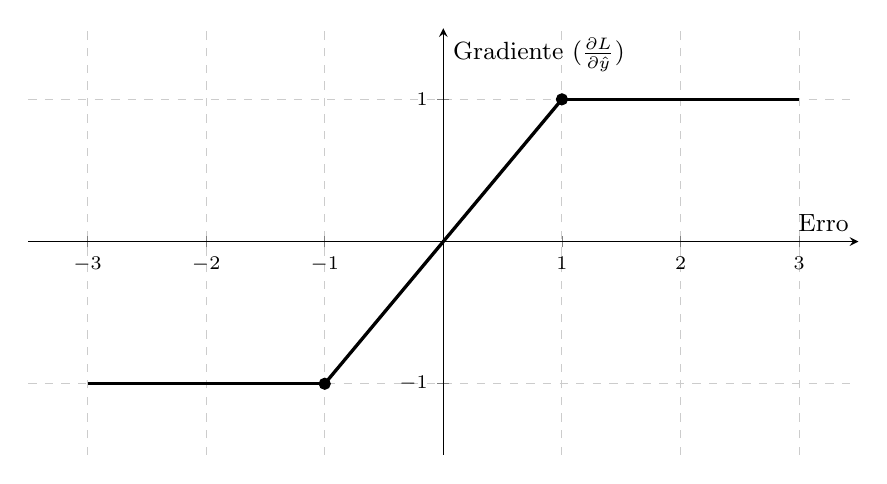
\begin{tikzpicture}
            \begin{axis}[
                % Dimensões ajustadas para caber lado a lado
                width=\linewidth, 
                height=7cm,
                xlabel={Erro},
                ylabel={Gradiente ($\frac{\partial L}{\partial \hat{y}}$)},
                axis lines=middle,
                grid=major,
                grid style={dashed, gray!40},
                xmin=-3.5, xmax=3.5,      % Limites do gráfico (além de delta)
                ymin=-1.5, ymax=1.5,      % Limites (um pouco além de -delta e +delta)
                ytick={-1, 0, 1},         % Ticks em -delta, 0, +delta
                xtick={-3, -2, -1, 0, 1, 2, 3}, % Ticks incluindo -delta e +delta
                legend pos=north west,
                title style={font=\bfseries\small},
                label style={font=\small},
                tick label style={font=\scriptsize}
            ]
                % Parte constante negativa (e < -delta)
                \addplot[
                    domain=-3:-1, 
                    samples=10, 
                    color=black,  
                    very thick
                ] {-1};
                \addplot[
                    domain=-1:1, 
                    samples=10, 
                    color=black, 
                    very thick
                ] {x}; % Valor e
                \addplot[
                    domain=1:3, 
                    samples=10, 
                    color=black, 
                    very thick 
                ] {1}; 
                \addplot[only marks, mark=*, color=black, mark size=2pt] coordinates {(-1,-1) (1,1)};
            \end{axis}
        \end{tikzpicture}
        \caption{Relação híbrida entre erro e gradiente da perda ($\text{Erro} =  y_j - \hat{y}_j$).}%
        \label{fig:huber-derivada-2d}
    \end{subfigure}
    \hfill 
    \begin{subfigure}[b]{0.48\textwidth}
        \centering
        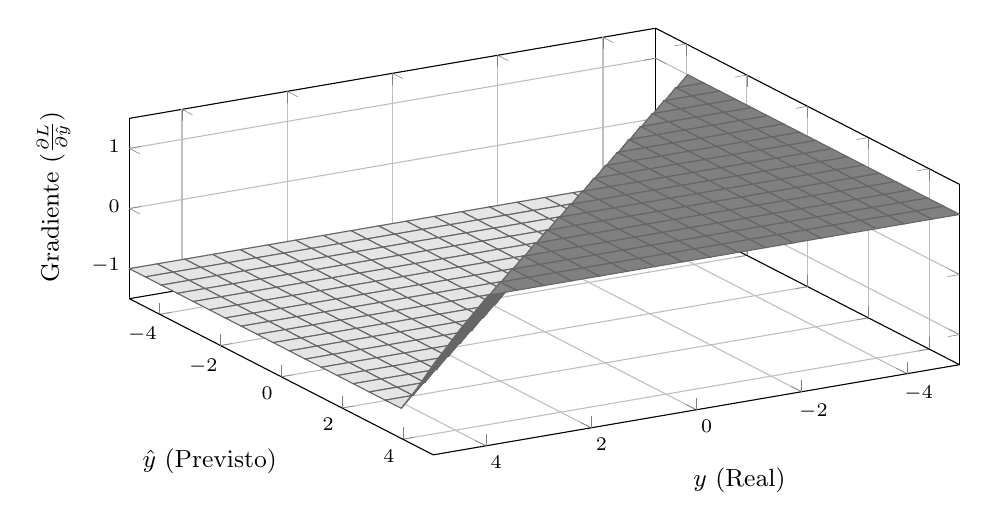
\begin{tikzpicture}
            \begin{axis}[
                % Dimensões consistentes com o gráfico (a)
                width=\linewidth,
                height=7cm,
                xlabel={$y$ (Real)},
                ylabel={$\hat{y}$ (Previsto)},
                zlabel={Gradiente ($\frac{\partial L}{\partial \hat{y}}$)},
                grid=major,
                view={150}{45}, % Mesmo ângulo de visão do seu template
                zmin=-1.5, zmax=1.5, % Espelha o eixo Y do gráfico 2D
                ztick={-1, 0, 1}, % Consistente com o 2D
                title style={font=\bfseries\small},
                label style={font=\small},
                tick label style={font=\scriptsize},
                colormap={bw}{gray(0cm)=(0.9); gray(1cm)=(0.5)}
            ]
                \addplot3[
                    surf,           
                    shader=faceted,  
                    faceted color=black!60, 
                    domain=-5:5,    
                    domain y=-5:5,  
                    samples=20,     
                    z buffer=sort       
                ] { ( abs(y-x) <= 1 ? (y-x) : (1 * sign(y-x)) ) }; 
            \end{axis}
        \end{tikzpicture}
        \caption{Superfície do gradiente no espaço.}%
        \label{fig:huber-derivada-3d}
    \end{subfigure}

    \caption{Visualizações da derivada (gradiente) da função de perda Huber (com $\delta = 1.0$).}%
    \label{fig:huber-derivada}
    \fonte{O autor (2025).}
\end{figure}

\subsubsection*{Aplicações da perda de Huber}%
\index{Aplicações práticas! Perda de Huber}

\begin{description}[style=sameline, leftmargin=1.5em, font=\bfseries\color{black}] 
    \item[Previsão de custos (Saúde):] \textcite{HuberLossSuperLearner} desenvolvem um algoritmo de \textit{ensemble} chamado de \textit{Super Leaner} com objetivo de prever custos para a área da saúde. Os autores usam a perda de Huber como função de perda do modelo \parencite{HuberLossSuperLearner}.
    \item[Visão computacional de veículos autônomos (Automotiva):] \textcite{RobustAleatoricModelingVehicleLocalization} apresentam uma rede \textit{feedforward} para previsão robusta para fazer a localização de objetos com intuito de ser utilizada em veículos autônomos. Os autores adotam a perda de Huber como função de perda para o modelo, como justificativa, eles explicam que ela apresenta a capacidade de treinar modelos de forma robusta contra caixas delimitadoras de referência (\textit{ground-truth}) anormais ou discrepantes.
    \item[Filtragem de tendências (Área):] \textcite{RobustTrendHuberLoss} discutem um novo algoritmo de filtragem de tendências em séries temporais, o objetivo é extrair o sinal de tendência de uma série temporal mesmo quando houver \textit{outliers} ou variações abruptas na tendência. Eles utilizam a perda de Huber como a função de perda escolhida para ser otimizada \parencite{RobustTrendHuberLoss}.
    \item[Aplicação 4 (Área):] \textcite{AdaptiveHuberRegression} propõem uma mudança no parâmetro de robustez da perda de Huber, o qual antes era fixo e agora passa a ser variável, considerando o tamanho da amostra, dimensão dos dados e outros parâmetros.
\end{description}

\medskip

A perda de Huber consegue unir o melhor dos dois mundos quando trata-se das perdas MSE e MAE. É uma função que atua de forma quadrática até certo ponto e depois, de forma linear. Ela garante ser robusta a \textit{outliers}, uma excelente vantagem para essa função. Entretanto, ao utilizar um parâmetro $\delta$ para definir o comportamento da função, a perda de Huber aumenta a complexidade do modelo criado. Esse fato pode ser um empecilho, gerando mais hiperparâmetro para ser otimizado empiricamente, levando mais tempo de pesquisa. Uma solução para manter o comportamento híbrido da perda, mas, ainda diminuir o hiperparâmetro de robustez, é a perda log-cosh.

\subsection{Perda log-cosh (log-cosh loss)}%
\index{Funções de Perda!Perda log-cosh (log-cosh loss)}%
\label{sec:log-cosh-loss}

A \textbf{perda log-cosh} é uma função de perda que vem ganhando popularidade entre os desenvolvedores. Em \textit{Statistical Properties of the log-cosh Loss Function Used in Machine Learning}, \textcite{StatisticalPropetiesLogCosh} explicam que ela aparece em cenários de \textit{autoencoders} variacionais, detecção de câncer, algoritmos de aprendizado baseados em árvores (como o XGBoost) e também em regressão quantílica (\textit{quantile regression}).

A fórmula da perda log-cosh está na Equação~\ref{eq:log-cosh-loss}. Se considerarmos o erro como sendo a diferença do valor real $y_j$ com o valor predito $\hat{y}_j$, a perda log-cosh é dada então pelo logaritmo natural do cosseno hiperbólico do erro.

\begin{equacaodestaque}{Perda log-cosh}
    \Loss_{\text{Log-Cosh}} (y_j, \hat{y}_j) = \sum_{j=1}^{N} \log(\cosh(y_j -\hat{y}_j))%
    \label{eq:log-cosh-loss}
\end{equacaodestaque}

Em que:

\begin{description}[style=sameline, leftmargin=1.5em, font=\bfseries\color{black}]  
    \item[$y_j$] representa o valor real da j-ésima amostra;
    \item[ $\hat{y}_j$] representa o valor predito pelo modelo para a j-ésima amostra;
    \item[$N$] representa o número de amostras.
\end{description}

A elegância da perda log-cosh está na interação dessas duas funções. Para erros pequenos,  $\cosh (e) \approx 1 + e^2/2$, como $\log (1 +x) \approx x$, a função se aproxima de $e^2/2$. Ou seja, para erros pequenos, a função tem um comportamento quadrático, semelhante ao que acontece do erro quadrático médio. Já para erros grandes, $\cosh (e) \approx e^{\|e\|}/2$, ao ser aplicado o logaritmo, o resultado se simplifica para uma função linear, $\log e^{\|e\|} \approx e$. Isso garante uma função robusta a \textit{outliers} assim como o MAE. Dessa forma, a perda log-cosh apresenta a mesma natureza híbrida, quadrática-linear, da perda de Huber, sendo uma alternativa que não necessita de hiperparâmetros adicionais. 

Esse comportamento variável para calcular os erros também é evidenciado nas suas representações gráficas, como a Figura~\ref{fig:log-cosh-loss} aponta. Em testes realizados por \textcite{StatisticalPropetiesLogCosh}, a perda log-cosh foi comparada com a perda de Huber, e foi verificado que as estimativas dessas funções bem como os erros padrões apresentam resultados similares.

\begin{figure}[h!]
    \centering 

    \begin{subfigure}[b]{0.48\textwidth}
        \centering
        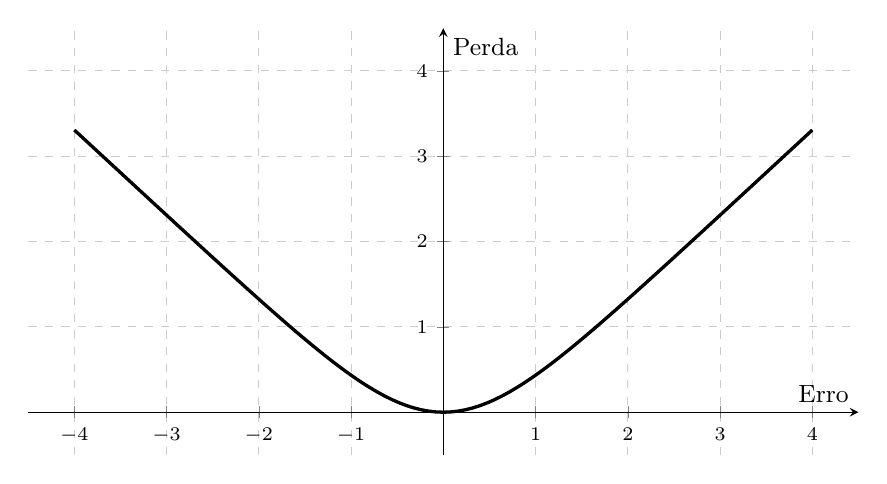
\begin{tikzpicture}
            \begin{axis}[
                % Dimensões ajustadas para caber lado a lado
                width=\linewidth,  
                height=7cm,
                xlabel={Erro},
                ylabel={Perda},
                axis lines=middle,
                grid=major,
                grid style={dashed, gray!40},
                xmin=-4.5, xmax=4.5,        % Limites do seu gráfico
                ymin=-0.5, ymax=4.5,         % Limites do seu gráfico
                legend pos=north west,
                title style={font=\bfseries\small},
                label style={font=\small},
                tick label style={font=\scriptsize}
            ]
                % Gráfico da função ln(cosh(x))
                \addplot[
                    domain=-4:4, 
                    samples=101,
                    color=black,  
                    very thick
                ] {ln(cosh(x))};
            \end{axis}
        \end{tikzpicture}
        \caption{Vista da função de perda em relação ao erro ($\text{Erro} =  y_j - \hat{y}_j$).}%
        \label{fig:log-cosh-2d}
    \end{subfigure}
    \hfill 
    \begin{subfigure}[b]{0.48\textwidth}
        \centering
        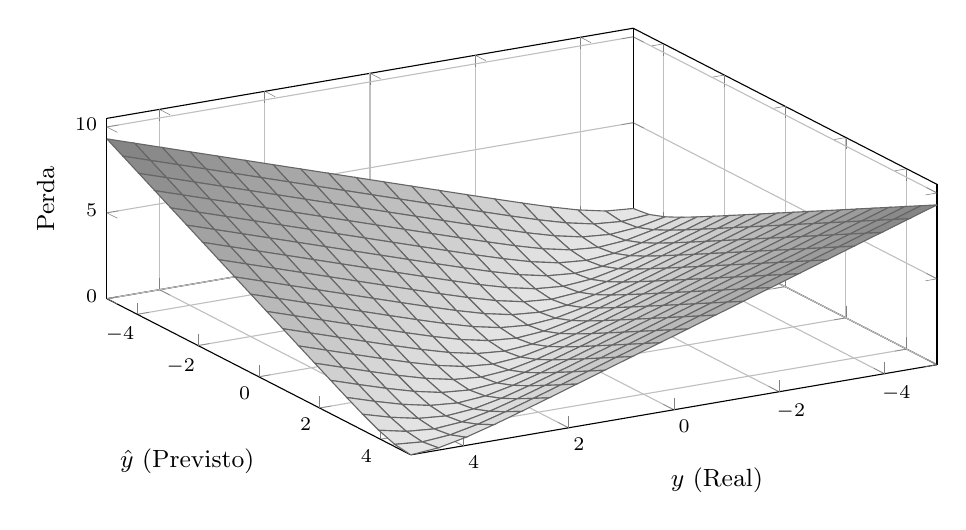
\begin{tikzpicture}
            \begin{axis}[
                width=\linewidth,
                height=7cm,
                xlabel={$y$ (Real)},
                ylabel={$\hat{y}$ (Previsto)},
                zlabel={Perda},
                grid=major,
                view={150}{45}, 
                zmin=0, zmax=10.5,
                title style={font=\bfseries\small},
                label style={font=\small},
                tick label style={font=\scriptsize},
                colormap={bw}{gray(0cm)=(0.9); gray(1cm)=(0.5)}
            ]
                \addplot3[
                    surf,           
                    shader=faceted,  
                    faceted color=black!60, 
                    domain=-5:5,    
                    domain y=-5:5,  
                    samples=20,     
                    z buffer=sort
                ] { ln(cosh(x - y)) }; % A função Log-Cosh 3D
            \end{axis}
        \end{tikzpicture}
        \caption{Superfície da função de perda.}%
        \label{fig:log-cosh-3d}
    \end{subfigure}

    % --- Legenda e Fonte da Figura Principal ---
    \caption{Visualizações da função de perda log-cosh em duas e em três dimensões.}%
    \label{fig:log-cosh-loss}
    \fonte{O autor (2025).}
\end{figure}

\subsubsection*{Características da perda log-cosh}

\begin{description}[style=sameline, leftmargin=1.5em, font=\bfseries\color{black}] 
    \item[Continuidade, suavidade e diferenciabilidade:] A perda log-cosh é uma função de classe $C^{\infty}$, infinitamente diferenciável, (ver Apêndice~\ref{ap:deducoes-log-cosh}). Isso é uma vantagem quando comparada com a perda de Huber, que é de classe $C^1$. Como consequência, a derivada da perda log-cosh é contínua em todo seu domínio. Esse fato pode ser útil caso essa função seja trabalhada em métodos de otimização de segunda ordem, que dependem do cálculo da matriz hessiana.
    \item[Convexidade:] A perda log-cosh é uma função estritamente convexa (ver Apêndice~\ref{ap:deducoes-log-cosh}). Isso é evidenciado ao calcular a segunda derivada dessa função, que tem como resultado $\frac{1}{\cosh^2(e)}$ que é estritamente positivo. Essa convexidade pode ser afetada ao trabalhar com modelos de aprendizado profundo, bem como as outras funções de perda.
    \item[Robustez a \textit{outliers}:] NA perda log-cosh é Lipschitz-contínua (ver Apêndice~\ref{ap:deducoes-log-cosh}). Isso decorre de sua derivada, $\tanh(x)$, que tem limite em 1. Assim, também é dito que a perda log-cosh é 1-Lipschitz-contínua. Como consequência, essa função é robusta a \textit{outliers} e portanto, ajuda a minimizar problemas de gradientes explosivos.
    \item[Alternativa para a perda de Huber:] Como dito anteriormente, a perda log-cosh é uma função híbrida assim como a perda de Huber. Ao escolher a perda log-cosh ao invés da perda de Huber para criar um algoritmo estamos priorizando a sua simplicidade, evitando o uso de hiperparâmetros que podem ser desnecessários e de difícil ajuste. Contudo, a perda de Huber ainda é essencial para aqueles casos em que queremos o controle total de como o erro será avaliado pela função de perda. Assim, chega-se em um dilema entre escolher a \textbf{simplicidade (perda log-cosh)} ou o \textbf{controle (perda de Huber)}.
\end{description}

\subsubsection*{Gradiente da perda de log-cosh}

A elegância da perda log-cosh não se restringe à sua função, estando presente também na sua derivada, a qual é dada pela tangente hiperbólica. Para encontrá-la, basta calcular a regra da cadeia dessa função de perda, de modo que seu resultado é

\[
    \frac{d}{de} \log(\cosh(e)) = \frac{1}{\cosh(e)} \cdot \sinh (e) 
\]

que se simplifica para o cálculo da tangente hiperbólica.

Assim, expandindo o cálculo da derivada para o cenário em duas dimensões, chega-se na Equação~\ref{eq:log-cosh-derivada}.

\begin{equacaodestaque}{Derivada parcial da perda log-cosh em relação à predição}
    \frac{\partial\Loss_{\text{log-cosh}}}{\partial\hat{y}_j} = \tanh(\hat{y}_j - y_j)%
    \label{eq:log-cosh-derivada}
\end{equacaodestaque}

Caso você tenha lido o Capítulo~\ref{cap:ativacao-sigmoidais}, pode ter notado que a tangente hiperbólica passa a assumir um novo papel além de uma função de ativação. Neste caso, ela serve para calcular o gradiente inicial.

Os gráficos da derivada parcial da perda log-cosh, vistos na Figura~\ref{eq:log-cosh-derivada}, servem de referência para entender o porquê desta função de perda ser robusta a \textit{outliers}. Como a tangente hiperbólica é limitada em um intervalo $\pm 1$, mesmo que o erro do modelo seja muito grande em termos de valores, a ``correção'' (representada pelo gradiente) não irá aumentar drasticamente. Vale destacar também que como a tangente hiperbólica retorna tanto valores negativos quanto positivos, isso também ajuda a garantir uma convergência mais rápida para os pontos de mínimo\footnote{Esse fato está evidenciado no Capítulo~\ref{cap:ativacao-sigmoidais}.}.

\begin{figure}[h!]
    \centering
    \begin{subfigure}[b]{0.48\textwidth}
        \centering
        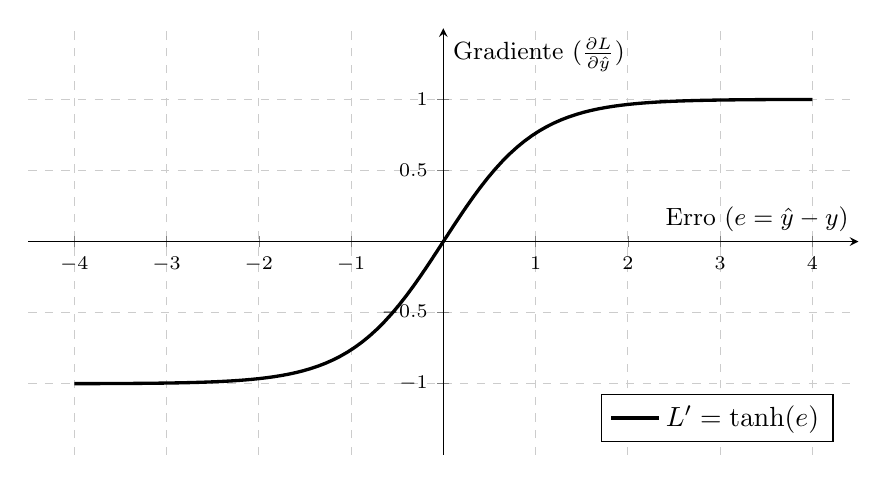
\begin{tikzpicture}
            \begin{axis}[
                width=\linewidth,  
                height=7cm,
                xlabel={Erro ($e = \hat{y} - y$)},
                ylabel={Gradiente ($\frac{\partial L}{\partial \hat{y}}$)},
                axis lines=middle,
                grid=major,
                grid style={dashed, gray!40},
                xmin=-4.5, xmax=4.5,   
                ymin=-1.5, ymax=1.5,       
                ytick={-1, -0.5, 0, 0.5, 1},
                legend pos=south east,
                title style={font=\bfseries\small},
                label style={font=\small},
                tick label style={font=\scriptsize}
            ]
                \addplot[
                    domain=-4:4, 
                    samples=101,
                    color=black, 
                    very thick
                ] {tanh(x)};
                
                \addlegendentry{$L' = \tanh(e)$}
            \end{axis}
        \end{tikzpicture}
        \caption{Relação harmônica entre erro e gradiente da perda.}%
        \label{fig:log-cosh-derivada-2d}
    \end{subfigure}
    \hfill 
    \begin{subfigure}[b]{0.48\textwidth}
        \centering
        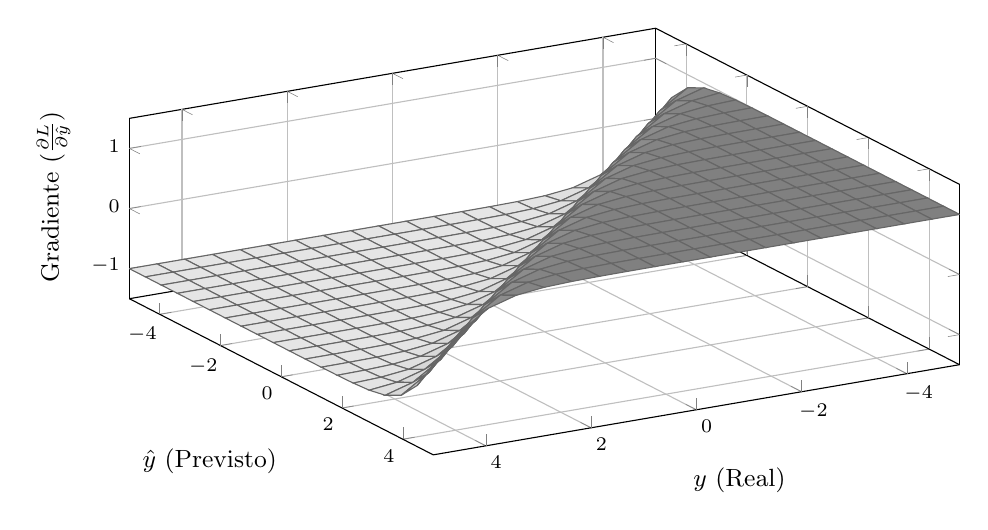
\begin{tikzpicture}
            \begin{axis}[
                width=\linewidth,
                height=7cm,
                xlabel={$y$ (Real)},
                ylabel={$\hat{y}$ (Previsto)},
                zlabel={Gradiente ($\frac{\partial L}{\partial \hat{y}}$)},
                grid=major,
                view={150}{45}, 
                zmin=-1.5, zmax=1.5, 
                ztick={-1, 0, 1},
                title style={font=\bfseries\small},
                label style={font=\small},
                tick label style={font=\scriptsize},
                colormap={bw}{gray(0cm)=(0.9); gray(1cm)=(0.5)}
            ]
                \addplot3[
                    surf,           
                    shader=faceted,  
                    faceted color=black!60, 
                    domain=-5:5,    
                    domain y=-5:5,  
                    samples=20,     
                    z buffer=sort
                ] { tanh(y - x) };
            \end{axis}
        \end{tikzpicture}
        \caption{Superfície do gradiente no espaço.}%
        \label{fig:log-cosh-derivada-3d}
    \end{subfigure}

    \caption{Visualizações do gradiente da perda log-cosh em relação à predição.}%
    \label{fig:log-cosh-derivada}
    \fonte{O autor (2025).}
\end{figure}

\subsubsection*{Aplicações da perda log-cosh}%
\index{Aplicações práticas! Perda log-cosh}

\begin{description}[style=sameline, leftmargin=1.5em, font=\bfseries\color{black}] 
    \item[Previsão de índices do mercado financeiro (Economia):] \textcite{FinantialMarketForecastingUsingRNN} criam algoritmos de aprendizado de máquina prever índices de ações globais (como o FTSE 100, S\&P 500 e HSI), construindo diferentes modelos, como uma rede neural recorrente. Eles utilizam a perda Log-Cosh junto com o MAE, o MSE, a RMSE e também a perda de Huber \parencite{FinantialMarketForecastingUsingRNN}.
    \item[Predição de bioatividade em moléculas (Farmácia):] \textcite{SiameseRecurrentNeuralNetwork} apresentam uma rede neural recorrente siamesa com o intuito de prever a bioatividade de pequenas moléculas. Os autores argumentam que a perda Log-Cosh foi uma função de perda ideal para ser aplicada nesse problema, pois apresentou o melhor desempenho das perdas que foram testadas: perda constrativa (\textit{constractive loss}), perda de Huber, perda L1 e perda L2 \parencite{SiameseRecurrentNeuralNetwork};
    \item[Aplicação 3 (Área):] \textcite{AnEffectiveMethodForDetectingUnknowTypes} propõem um modelo de \textit{deep learning} chamado de \textit{LVAE (Log-Cosh Variational Autoencoder)} com intuito detectar tipos desconhecidos de ataques em redes. A perda log-cosh é utilizada como a função de perda de reconstrução dentro do modelo \textit{variational autoencoder} \parencite{AnEffectiveMethodForDetectingUnknowTypes}.
\end{description}

\medskip

Todas as funções de perda vistas até o momento calculam o erro de forma absoluta. Elas não lidam com o erro de forma relativa. Como consequência, um erro de R\$ $50,00$ em uma conta de padaria tem o mesmo grau que um erro da mesma magnitude para validar o aluguel de uma casa. Para os casos em que deve-se considerar o erro de forma relativa, cabe analisar outras funções, como o erro quadrático logarítmico médio ou a perda quantílica.

\section{Lidando com a escala: foco no erro relativo}

\subsubsection*{O problema dos imóveis}

Considere que existem duas situações que está sendo previsto os valores de imóveis:

\begin{description}[style=sameline, leftmargin=1.5em, font=\bfseries\color{black}] 
    \item[Cenário A:] o modelo previu que uma casa vale 50.000 R\$. Enquanto no rótulo está que ela vale 100.000 R\$.
    \item[Cenário B:] o modelo previu que uma casa vale 950.000 R\$. Enquanto no rótulo está que ela vale 1.000.000 R\$..
\end{description}

Utilizando o MSE para calcular a perda dessas funções encontramos que o erro será de $50.000$ e a perda de $250.00.000$, independentemente dos cenários. Para o cenário B, a previsão do modelo não foi tão ruim, foi uma previsão realista. Contudo, o modelo do cenário A previu que a casa valia apenas a metade do seu valor real, ele fez uma previsão subestimada.

Neste caso, avaliar os modelos com uma função de perda que calcula o erro de forma absoluta (como o MSE e o MAE), pode não ser ideal. Para evitar esses problemas de subestimação, uma solução é o erro quadrático médio logarítmico.

\subsection{Erro quadrático médio logarítmico (MSLE)}%
\index{Funções de Perda!Erro quadrático médio logarítimico (MSLE)}%

O \textbf{erro quadrático médio logarítmico}, também chamado de \textbf{\textit{mean squared logarithmic error}} (\textbf{MSLE}), é calculado pela Equação~\ref{eq:msle-loss}. Ele calcula o erro como sendo a diferença dos logaritmos naturais do valor real $y_j$ com a predição $\hat{y}_j$ e depois faz a média dos erros das diferentes previsões.

\begin{equacaodestaque}{Erro quadrático médio logarítmico}
    \Loss_{\text{MSLE}} (y_j, \hat{y}_j) = \frac{1}{N} \sum_{j=1}^{N} (\ln(y_j + 1) -\ln(\hat{y}_j + 1))^2%
    \label{eq:msle-loss}
\end{equacaodestaque}

Em que:

\begin{description}[style=sameline, leftmargin=1.5em, font=\bfseries\color{black}]  
    \item[$y_j$] representa o valor real da j-ésima amostra;
    \item[ $\hat{y}_j$] representa o valor predito pelo modelo para a j-ésima amostra;
    \item[$N$] representa o número de amostras.
\end{description}

O valor $1$ que é somado junto com os valores de entrada no logaritmo serve como forma de evitar que seja calculado o logaritmo de zero, que não existe no conjunto dos reais. 

A Figura~\ref{fig:msle-loss} evidencia a natureza assimétrica do erro quadrático logarítmico. Para as situações em que a previsão $\hat{y}_j$ tem um valor muito pequeno quando comparada ao valor real $y_j$ a distância entre esses dois pontos é consideravelmente maior devido ao comportamento dos logaritmos. Dessa forma, para subestimações, o MSLE gera erros maiores. Isso é útil para resolver o problema das contas de padaria e também de preços de imóveis vistos anteriormente. 

\begin{figure}[h!]
    \centering 

    \begin{subfigure}[b]{0.48\textwidth}
        \centering
        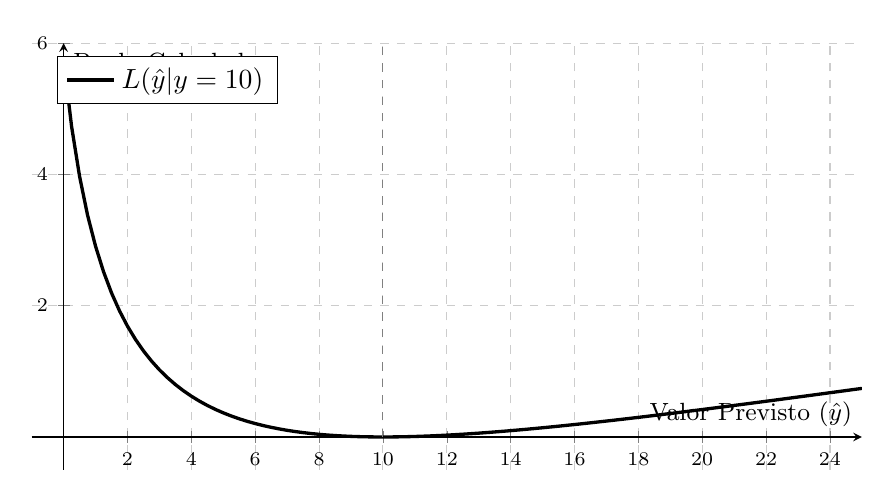
\begin{tikzpicture}
            \begin{axis}[
                % Dimensões ajustadas para caber lado a lado
                width=\linewidth,  
                height=7cm,
                xlabel={Valor Previsto ($\hat{y}$)},
                ylabel={Perda Calculada},
                axis lines=middle,
                grid=major,
                grid style={dashed, gray!40},
                xmin=-1, xmax=25,        % Limites do seu gráfico
                ymin=-0.5, ymax=6,         % Limites do seu gráfico
                legend pos=north west,
                title style={font=\bfseries\small},
                label style={font=\small},
                tick label style={font=\scriptsize}
            ]
                % Gráfico da função (ln(11) - ln(x+1))^2
                \addplot[
                    domain=0:25, 
                    samples=101,
                    color=black, 
                    very thick
                ] {(ln(10+1) - ln(x+1))^2};
                
                \addlegendentry{$L(\hat{y} | y=10)$}

                % Linha vertical para marcar o valor real
                \draw[dashed, gray] (axis cs:10, 0) -- (axis cs:10, 6);
                \node[above, gray!80, font=\tiny] at (axis cs:10, 6) {Valor Real ($y=10$)};
            \end{axis}
        \end{tikzpicture}
        \caption{Vista da função de perda em relação ao erro.}%
        \label{fig:msle-2d}
    \end{subfigure}
    \hfill 
    \begin{subfigure}[b]{0.48\textwidth}
        \centering
        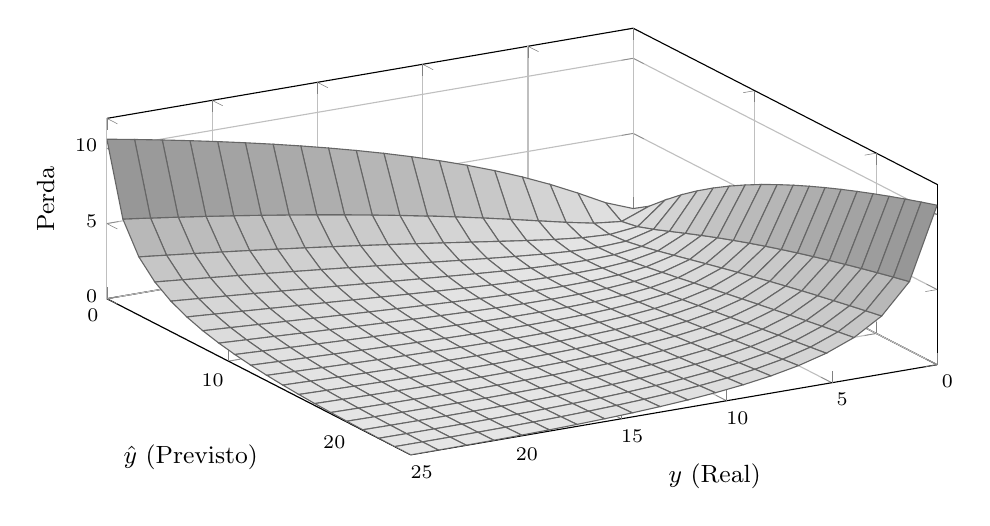
\begin{tikzpicture}
            \begin{axis}[
                % Dimensões consistentes com o gráfico (a)
                width=\linewidth,
                height=7cm,
                xlabel={$y$ (Real)},
                ylabel={$\hat{y}$ (Previsto)},
                zlabel={Perda},
                grid=major,
                view={150}{45}, % Mesmo ângulo de visão do seu template
                zmin=0, zmax=12, % Ajustado para (ln(26)-ln(1))^2
                title style={font=\bfseries\small},
                label style={font=\small},
                tick label style={font=\scriptsize},
                colormap={bw}{gray(0cm)=(0.9); gray(1cm)=(0.5)}
            ]
                % Gráfico da superfície da MSLE
                \addplot3[    
                    surf,     
                    shader=faceted,  
                    faceted color=black!60, 
                    domain=-0:25,    
                    domain y=-0:25,  
                    samples=20,     
                    z buffer=sort
                ] { (ln(x+1) - ln(y+1))^2 }; % A função MSLE 3D
            \end{axis}
        \end{tikzpicture}
        \caption{Superfície da função de perda.}%
        \label{fig:msle-3d}
    \end{subfigure}

    \caption{Visualizações da função de perda erro quadrático médio logarítmico.}%
    \label{fig:msle-loss}
    \fonte{O autor (2025).}
\end{figure}

Essa propriedade assimétrica dos logaritmos também é explorada ao descrever o comportamento da entropia cruzada binária e funções semelhantes (vistas com mais detalhes do Capítulo~\ref{cap:perda-classificacao}). Neste caso, a forma com que a função utiliza os logaritmos faz com que sejam punidas em maior peso as previsões confiantes que estão erradas.

\subsubsection*{Características do erro quadrático médio logarítmico}

\begin{description}[style=sameline, leftmargin=1.5em, font=\bfseries\color{black}] 
    \item[Continuidade, suavidade e diferenciabilidade:] O MSLE é uma função de classe $C^{\infty}$ (infinitamente diferenciável) (ver Apêndice~\ref{ap:deducoes-msle}). Isso contribui para uma função de perda que pode ser facilmente utilizada em conjunto com otimizadores baseados em gradiente, dado que não serão encontrados problemas de continuidade ao derivar essa função.
    \item[Convexidade:] A função MSLE é convexa em relação à predição transformada $z = \log(1+\hat{y})$, mas não é globalmente convexa em relação a $\hat{y}$ (ver Apêndice~\ref{ap:deducoes-msle}). 
    \item[Robustez:] A função MSLE é Lipschitz-contínua, portanto é robusta a \textit{outliers} (ver Apêndice~\ref{ap:deducoes-msle}). Diferente do erro absoluto médio, que quando o valor do erro ``explode'' para infinito o seu gradiente será 1, no MSLE o seu gradiente tende a 0. Como resultado, para erros muito grandes o erro logarítmico médio gera uma correção irrisória, o que pode não ser útil em certos casos.
    \item[Foco no erro relativo (percentual):] Quando o MSLE é utilizado como função de perda, diferente das outras vistas até agora que medem o erro absoluto, o erro quadrático logarítmico médio mede o erro percentual/relativo. Isso acontece por conta dos uso dos logaritmos dessa função, que são responsáveis por comprimir a escala dos dados. Portanto, erros em que o valor predito é 50\% menor que o real são mais penalizados em que cenários nos quais o valor predito é 5\% menor;
    \item[Tendência de penalizar subestimações:] Como aponta a Figura~\ref{fig:msle-loss}, o MSLE não forma uma curva convexa simétrica verticalmente, conforme os valores vão diminuindo, a perda aumenta consideravelmente. Enquanto isso, conforme os valores aumentam, a perda também aumenta, mas não de forma tão agressiva quanto no sentido inverso. Isso significa que quanto maior for a diferença entre o valor previsto $\hat{y}_j$ e o valor real $y_j$, existe uma tendência de que a perda será maior;
    \item[Restrição de domínio (não-negatividade):] Como os logaritmos são indeterminados para valores nulos ou negativos, o MSLE exige que os valores de entrada sejam positivos ($y_j > 0$ e $\hat{y}_j > 0$). Caso os conjunto de dados contenha valores negativos (como lucro/prejuízo ou temperaturas), o MSLE irá causar erros matemáticos. Para contornar esse problema, deve-se aplicar uma transformação nos dados, como somar uma constante para deslocar os valores negativos para positivos, ou ser utilizada outra função de perda.
\end{description}

\subsubsection*{Gradiente do erro quadrático médio logarítmico}

Na equação~\ref{eq:msle-derivada} está a derivada do erro quadrático médio logarítmico em relação os valores preditos pelo modelo $\hat{y}_j$.

\begin{equacaodestaque}{Derivada parcial do erro quadrático médio logarítmico em relação à predição}
    \frac{\partial\Loss_{\text{MSLE}}}{\partial\hat{y}_j} (y_j, \hat{y}_j) = -\frac{2}{N} \cdot \frac{\ln(y_j + 1) -\ln(\hat{y}_j + 1)}{\hat{y}_j + 1}%
    \label{eq:msle-derivada}
\end{equacaodestaque}
 
O comportamento assimétrico do MSLE também está presente nos gráficos da sua derivada vistos na Figura~\ref{fig:msle-derivada}. Eles mostram de forma intuitiva o tamanho da correção que será feita conforme o modelo vai errando durante suas predições. O canto esquerdo do gráfico da superfície da derivada mostra uma situação em que o modelo subestima os valores reais. Nesta parte, os valores do gradiente começam a subir de uma forma que lembra uma curva exponencial. 

\begin{figure}[h!]
    \centering 

    \begin{subfigure}[b]{0.48\textwidth}
        \centering
        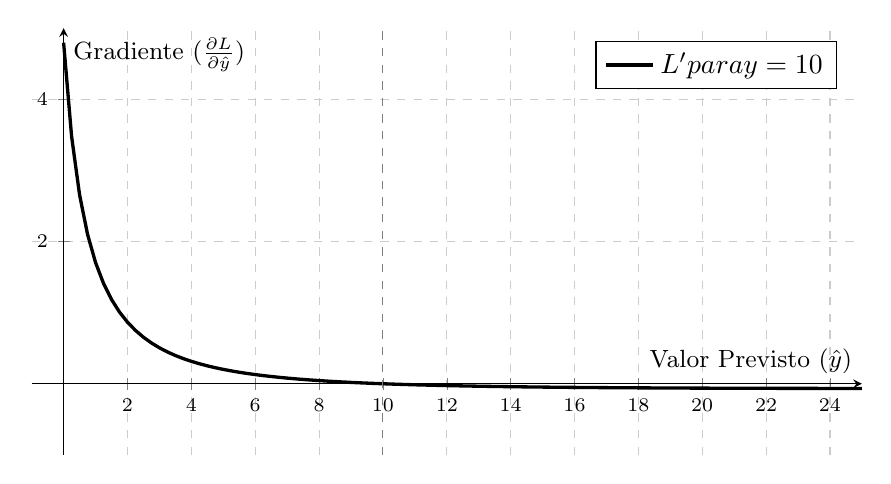
\begin{tikzpicture}
            \begin{axis}[
                width=\linewidth,  
                height=7cm,
                xlabel={Valor Previsto ($\hat{y}$)},
                ylabel={Gradiente ($\frac{\partial L}{\partial \hat{y}}$)},
                axis lines=middle,
                grid=major,
                grid style={dashed, gray!40},
                xmin=-1, xmax=25, 
                ymin=-1, ymax=5,      
                legend pos=north east,
                title style={font=\bfseries\small},
                label style={font=\small},
                tick label style={font=\scriptsize}
            ]
                
                \addplot[
                    domain=0:25, 
                    samples=101,
                    color=black, 
                    very thick
                ] {2 * (ln(10+1) - ln(x+1)) / (x+1)}; 
                
                \addlegendentry{$L' \text{ para } y=10$}

                \draw[dashed, gray] (axis cs:10, -1) -- (axis cs:10, 5);
                \node[above, gray!80, font=\tiny] at (axis cs:10, 5) {Valor Real};
            \end{axis}
        \end{tikzpicture}
        \caption{Relação assimétrica entre erro e gradiente da perda.}%
        \label{fig:msle-derivada-2d}
    \end{subfigure}
    \hfill 
    \begin{subfigure}[b]{0.48\textwidth}
        \centering
        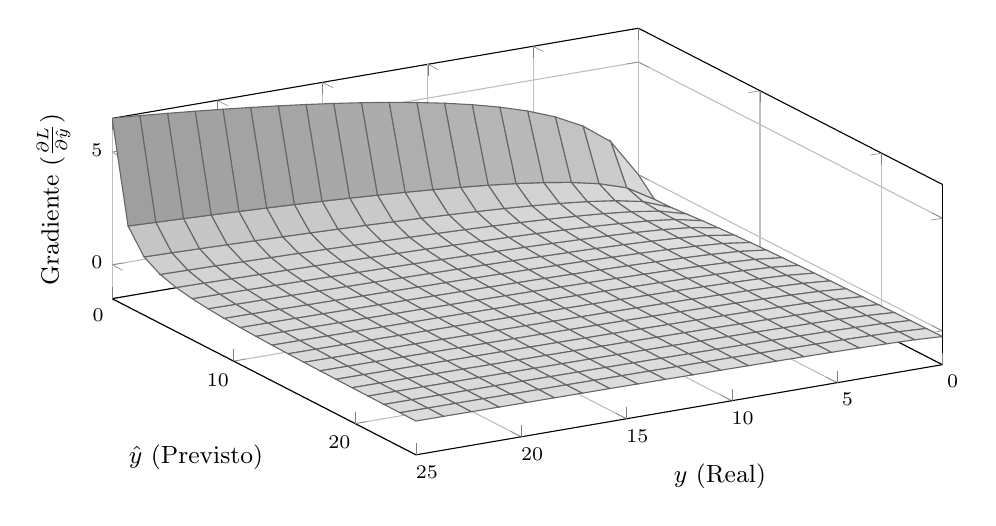
\begin{tikzpicture}
            \begin{axis}[
                width=\linewidth,
                height=7cm,
                xlabel={$y$ (Real)},
                ylabel={$\hat{y}$ (Previsto)},
                zlabel={Gradiente ($\frac{\partial L}{\partial \hat{y}}$)},
                grid=major,
                view={150}{45},
                zmin=-1.5, zmax=6.5,
                title style={font=\bfseries\small},
                label style={font=\small},
                tick label style={font=\scriptsize},
                colormap={bw}{gray(0cm)=(0.9); gray(1cm)=(0.5)}
            ]
                \addplot3[
                    surf,           
                    shader=faceted,  
                    faceted color=black!60, 
                    domain=-0:25,    
                    domain y=-0:25,  
                    samples=20,     
                    z buffer=sort
                ] { 2 * (ln(x+1) - ln(y+1)) / (y+1) };
            \end{axis}
        \end{tikzpicture}
        \caption{Superfície do gradiente no espaço.}%
        \label{fig:msle-derivada-3d}
    \end{subfigure}

    \caption{Visualizações do gradiente da perda log-cosh em relação à predição.}%
    \label{fig:msle-derivada}
    \fonte{O autor (2025).}
\end{figure}

\subsubsection*{O problema dos imóveis com o MSLE}

Voltando para o exemplo anterior dos modelos prevendo preços de imóveis. Cabe discutir como o MSLE se compara ao erro quadrático médio, e como ele pode ser uma alternativa para função de perda em cenários em que é preciso garantir que as subestimações sejam mais penalizadas.

Com esse intuito, a Tabela~\ref{tab:comparativo-mse-msle} compara os dois cenários vistos na seção anterior, e mostra qual foi o valor do erro calculado para essas situações.

\begin{table}[htbp]
    \centering
    \begin{threeparttable}
        \caption{Comparativo das funções de perda MSE e MSLE}%
        \label{tab:comparativo-mse-msle}
        \begin{tabular}{l c c c c }
            \toprule
            Cenário & $y_j$ (real) & $\hat{y}_j$ (predito) & MSE & MSLE \\
            \midrule
            Cenário A & $100.000$ & $50.000$ & $2.500.000.000$ & $0,4804$ \\
            Cenário B & $1.000.000$ & $950.000$ & $2.500.000.000$ & $0,0026$ \\
            \bottomrule
        \end{tabular}
        
        \begin{tablenotes}[para]
            \small
            \item[] Fonte: O autor (2025).
        \end{tablenotes}

    \end{threeparttable}
\end{table}

O erro quadrático médio considera a grandeza dos valores, nos dois cenários o erro é o mesmo. Consequentemente a atualização do gradiente, para o modelo os erros são de mesma magnitude. Contudo, olhando agora para os valores do MSLE, o cenário A, em que o modelo subestimou o valor do imóvel, é cerca de 185 vezes pior que o do cenário B. Neste caso, como no cenário A o erro foi maior, as atualizações nos parâmetros do modelo também serão maiores, enquanto no cenário B ainda irá ocorrer atualizações, mas como apontado, os valores dos parâmetros irão ter uma variação menor de uma época para a próxima.

\subsubsection*{Raiz do erro quadrático médio logarítmico (RMSLE)}

Do MSLE é possível derivar a métrica raiz do erro quadrático médio logarítmico (RMSLE) que também serve para avaliar problemas de predição. Neste caso, o RMSLE é dado pelo cálculo da raiz quadrada da função de perda RMSE.

\begin{equacaodestaque}{Raiz do erro quadrático médio logarítmico}
    \text{RMSLE} (y_j, \hat{y}_j) = \sqrt{\frac{1}{N} \sum_{j=1}^{N} (\log(y_j + 1) -\log(\hat{y}_j + 1))^2}%
    \label{eq:rmsle-metric}
\end{equacaodestaque}

Em que:

\begin{description}[style=sameline, leftmargin=1.5em, font=\bfseries\color{black}]  
    \item[$y_j$] representa o valor real da j-ésima amostra;
    \item[ $\hat{y}_j$] representa o valor predito pelo modelo para a j-ésima amostra;
    \item[$N$] representa o número de amostras.
\end{description}

Ao calcular a raiz quadrada do erro quadrático médio logarítmico tem-se uma noção melhor da magnitude dos erros, dado que eles são mascarados ao serem elevados ao quadrado pela expressão do RMSLE. Diante disso, a equação da raiz do erro quadrático médio logarítmico consegue melhorar a interpretabilidade dos erros, servindo como uma métrica que pode ser aplicada para problemas em que as subestimações devem ser mais penalizadas.

\subsubsection*{Aplicações do erro quadrático logarítmico médio}%
\index{Aplicações práticas! Erro quadrático logarítimico médio}

\begin{description}[style=sameline, leftmargin=1.5em, font=\bfseries\color{black}] 
    \item[Predição do preço de casas (Mercado imobiliário):] \textcite{SunKim-NetOverYourHead} desenvolvem uma rede neural para fazer a previsão do preço de casas. Eles utilizam como métrica o RMSLE, como justificativa, os autores explicam que o \textit{dataset} que está sendo utilizado apresenta casas que têm ordem de magnitude de diferença de preço, e com isso uma previsão ruim para uma casa de alto valor terá mais peso que uma previsão ruim para uma casa de baixo valor; ao usar o RMSLE é possível capturar as ordens de magnitude dos preços das casas, algo que não acontece com o RMSE \parencite{SunKim-NetOverYourHead};
    \item[Predição no tempo de internação de pacientes (Saúde):] \textcite{Winter2023PredictingLOS} analisam maneiras de prever o tempo de internação de um paciente qualquer após receber alta no pronto-socorro e sua transferência para a próxima unidade hospitalar. Os autores usam um modelo de regressão de \textit{gradient boosting} com arquitetura \textit{CatBoost}, para a função de perda, os autores escolhem duas, a primeira sendo o RMSE e a segunda o RMSLE, como justificativa, os autores apontam que o RMSLE penaliza erros proporcionais e é menos afetado por \textit{outliers};
    \item[Previsão de séries temporais (Área):] \textcite{Jadon2022ComprehensiveSurvey} analisam uma série de funções de perda que são comumente utilizadas na previsão de séries temporais, sendo uma delas o MSLE. Os autores apontam que o MSLE reduz o efeito punitivo de diferenças significativas em grandes valores previsos; sendo apropriado quando o modelo prevê quantidades não escalonadas diretamente \parencite{Jadon2022ComprehensiveSurvey}. \textcite{Jadon2022ComprehensiveSurvey} analisam também o RMSLE, explicando que ele pode ser uma função de perda para ser utilizada em cenários em que a subestimação dos valores reais não é aceitável, mas a superestimações do modelo não são consideradas um problema.
\end{description}

\medskip

O erro quadrático médio logarítmico médio penaliza fortemente as subestimações feitas pelo modelo. Entretanto, pode ser necessário uma função que tenha a característica contrária: penalizar em maior grau as superestimações. Dessa forma, uma solução é utilizar a perda quantílica.

\section{Mudando o objetivo da previsão: além da média}

Até agora todas as funções de perda vistas calculavam o erro para um conjunto $m$ de instâncias, e a partir disso aplicavam o cálculo da média dos erros. Ao calcular a média dos erros, está sendo presumido que a tendência central é a característica mais informativa daquela distribuição de dados, seguindo a clássica distribuição Gaussiana. Contudo, e quando isso não for a realidade? E quando a caraterística mais comum estiver deslocada mais para à esquerda (como na Figura~\ref{fig:dist-skew-esquerda}), ou mais para à direita da distribuição (como na Figura~\ref{fig:dist-skew-direita})?

\begin{figure}[h!]
    \centering 

    \begin{subfigure}[b]{0.48\textwidth}
        \centering
        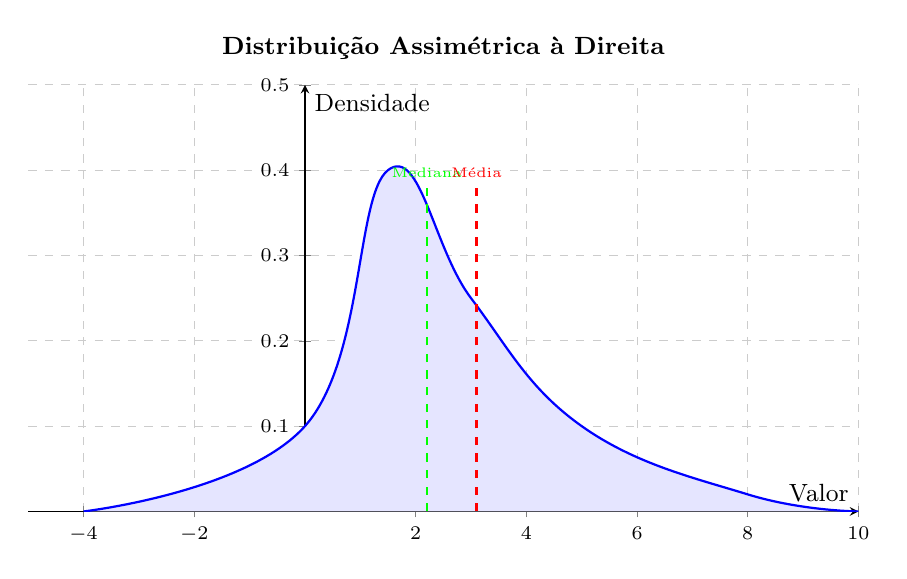
\begin{tikzpicture}
            \begin{axis}[
                width=\linewidth,
                height=7cm,
                xlabel={Valor},
                ylabel={Densidade},
                axis lines=middle,
                grid=major,
                grid style={dashed, gray!40},
                xmin=-5, xmax=10,
                ymin=0, ymax=0.5,
                legend pos=north west,
                title style={font=\bfseries\small},
                label style={font=\small},
                tick label style={font=\scriptsize},
                title={Distribuição Assimétrica à Direita}
            ]
                
                % Curva "desenhada" com smooth
                \addplot[
                    blue, thick, fill=blue!10,
                    smooth, tension=0.7 % 'tension' controla a suavidade
                ] coordinates {
                    (-4, 0)
                    (0, 0.1)
                    (1.5, 0.4)  % Pico (Moda)
                    (3, 0.25)
                    (5, 0.1)
                    (8, 0.02)
                    (10, 0)
                };

                % Mediana (mais perto do pico)
                \pgfmathsetmacro{\medianpos}{2.2} 
                \addplot[dashed, color=green, thick] coordinates {(\medianpos,0) (\medianpos,0.38)};
                \node[above, font=\tiny, green] at (axis cs:\medianpos,0.38) {Mediana};

                % Média (puxada pela cauda)
                \pgfmathsetmacro{\meanpos}{3.1} 
                \addplot[dashed, color=red, thick] coordinates {(\meanpos,0) (\meanpos,0.38)};
                \node[above, font=\tiny, red] at (axis cs:\meanpos,0.38) {Média};

            \end{axis}
        \end{tikzpicture}
        \caption{Assimétrica à direita (skew positivo).}%
        \label{fig:dist-skew-direita}
    \end{subfigure}
    \hfill 
    \begin{subfigure}[b]{0.48\textwidth}
        \centering
        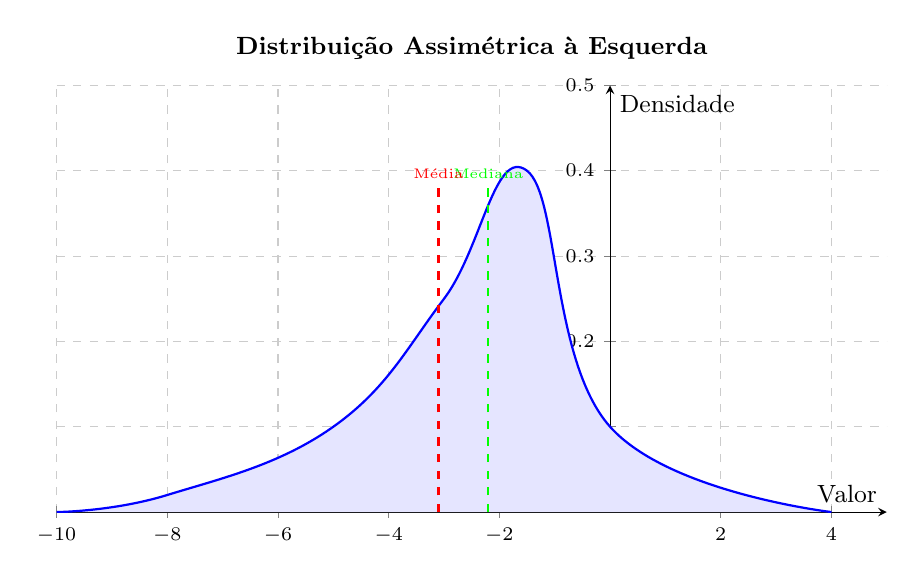
\begin{tikzpicture}
            \begin{axis}[
                width=\linewidth,
                height=7cm,
                xlabel={Valor},
                ylabel={Densidade},
                axis lines=middle,
                grid=major,
                grid style={dashed, gray!40},
                xmin=-10, xmax=5,
                ymin=0, ymax=0.5,
                legend pos=north east,
                title style={font=\bfseries\small},
                label style={font=\small},
                tick label style={font=\scriptsize},
                title={Distribuição Assimétrica à Esquerda}
            ]
                
                % Curva "desenhada" com smooth
                \addplot[
                    blue, thick, fill=blue!10,
                    smooth, tension=0.7
                ] coordinates {
                    (-10, 0)
                    (-8, 0.02)
                    (-5, 0.1)
                    (-3, 0.25)
                    (-1.5, 0.4) % Pico (Moda)
                    (0, 0.1)
                    (4, 0)
                };

                % Mediana (mais perto do pico)
                \pgfmathsetmacro{\medianneg}{-2.2} 
                \addplot[dashed, color=green, thick] coordinates {(\medianneg,0) (\medianneg,0.38)};
                \node[above, font=\tiny, green] at (axis cs:\medianneg,0.38) {Mediana};

                % Média (puxada pela cauda)
                \pgfmathsetmacro{\meannneg}{-3.1} 
                \addplot[dashed, color=red, thick] coordinates {(\meannneg,0) (\meannneg,0.38)};
                \node[above, font=\tiny, red] at (axis cs:\meannneg,0.38) {Média};

            \end{axis}
        \end{tikzpicture}
        \caption{Assimétrica à esquerda (skew negativo).}%
        \label{fig:dist-skew-esquerda}
    \end{subfigure}

    \caption{Exemplos de distribuições assimétricas (desenhadas) onde a média (vermelho) e a mediana (verde) divergem, justificando o uso da Perda Quantílica.}%
    \label{fig:distribuicoes-assimetricas}
    \fonte{O autor (2025).}
\end{figure}

A perda quantílica consegue lidar com as situações em que a média e a medina são divergentes. Ela foca em estudar como a perda acontece em diferentes quantis da distribuição. Ao utilizá-la, é definido o quantil que será analisado, escolhendo se ela irá funcionar de forma assimétrica, ou de forma parecida com o MAE.

A $\epsilon$-insensível também é outra função de perda que não faz o cálculo da média dos erros. Ela é uma função essencial para a tarefas de regressão para máquinas de vetores de suporte. Ao utilizá-la, é definido uma ``margem de tolerância'' em que caso o erro esteja dentro dessa média, a perda não irá penalizar o modelo.

\subsection{Perda quantílica (quantile loss)}%
\index{Funções de Perda!Perda quantílica (\textit{quantile loss})}

Em \textit{Regression Quantiles}, \textcite{regression-quantiles} analisaram uma nova técnica de regressão que se baseava nos quantis de uma distribuição. Como motivação, os autores discutem a ideia de que ``todos acreditam na lei de Gauss para os erros, porque eles acreditam que é um teorema matemático, e os matemáticos acreditam porque é um fato experimental'' \parencite{regression-quantiles}. Contudo, isso não é uma verdade absoluta, existem casos, como os vistos na introdução dessa seção, que fogem da distribuição normal. Como consequência, técnicas mais conhecidas, como o MSE, para o cálculo dos erros com base na média, não são ideais para servir de guia para a otimização do modelo.

Tendo isso em mente, os pesquisadores apresentam uma forma de minimizar a soma de perdas assimétricas, definindo a Equação~\ref{eq:soma-das-perdas-assimetricas}\footnote{Caso você leitor decida ler o artigo original dos pesquisadores, você verá um conjunto diferente de notações utilizadas, isso acontece pois neste livro elas foram adaptadas para condizer com as notações que já estavam sendo utilizadas anteriormente nos outros capítulos}.

\begin{equation}
    \Loss(w; \tau, y, X) = \sum_{j \text{ t.q. } y_j > \hat{y}_j} \tau |y_j -\hat{y}_j| + \sum_{j \text{ t.q. } y_j < \hat{y}_j} (1 -\tau) |y_j -\hat{y}_j|
    \label{eq:soma-das-perdas-assimetricas}
\end{equation}

Em que:

\begin{description}[style=sameline, leftmargin=1.5em, font=\bfseries\color{black}]  
    \item[$\tau$] representa o quantil;
    \item[ $w$] representa os parâmetros do modelo, neste caso, os pesos;
    \item[$y_j$] representa o valor real da j-ésima amostra;
    \item[ $\hat{y}_j$] representa o valor predito pelo modelo para a j-ésima amostra.
\end{description}

A partir da Equação~\ref{eq:soma-das-perdas-assimetricas}, é possível derivá-la em dois casos distintos. O caso em que o valor real é maior que a previsão $(y_j > \hat{y}_j)$, ou seja, ocorre uma subestimação, é gerado um erro positivo. Assim, a perda é proporcional a $\tau$. Quando o valor real é menor que a previsão $(y_j < \hat{y}_j)$, o modelo superestimou o valor real, é aplicado o peso $(1 - \tau)$. Desses dois cenários, deriva-se a definição por partes da \textbf{perda quantílica}, também conhecida como \textbf{\textit{quantile loss}}, dada pela Equação~\ref{eq:quantile-loss}. Neste caso, está sendo considerado que a situação $\hat{y} = y$ faz parte do primeiro caso estudado.

\begin{equacaodestaque}{Perda quantílica}
    \Loss_{\tau} (y_j, \hat{y}_j) = 
    \begin{cases} 
        \tau(y_j -\hat{y}_j) & \text{se } y_j \ge \hat{y}_j\\
        (1 -\tau) (\hat{y}_j -y_j) & \text{se } y_j < \hat{y}_j\end{cases}%
    \label{eq:quantile-loss}
\end{equacaodestaque}

Em que:

\begin{description}[style=sameline, leftmargin=1.5em, font=\bfseries\color{black}]  
    \item[$y_j$] representa o valor real da j-ésima amostra;
    \item[$\hat{y}_j$] representa o valor predito pelo modelo;
    \item[$\tau$] representa o quantil.
\end{description}

Existem também uma versão compacta da perda quantílica, presente na Equação~\ref{eq:quantile-loss-com-max}, ela utiliza a função $\max$ para definir a função por partes em apenas uma linha.

\begin{equacaodestaque}{Perda quantílica com $\max$}
    \Loss_{\tau} (e)= \max(\tau e, (\tau-1 )e)%
    \label{eq:quantile-loss-com-max}
\end{equacaodestaque}

Considerando que $e = y - \hat{y}$, ou seja, o cálculo do erro.

A perda quantílica com $\tau = 0,5$ é retratada na Figura~\ref{fig:quantile-loss-tau05}. Os gráficos são semelhantes ao erro absoluto médio, porque o MAE é uma função que analisa justamente o quantil 0,5. Assim, não faz muito sentido utilizar a perda quantílica para esse cenário em específico, considerando que já existe uma função com essa finalidade.

\begin{figure}[h!]
    \centering 

    \begin{subfigure}[b]{0.48\textwidth}
        \centering
        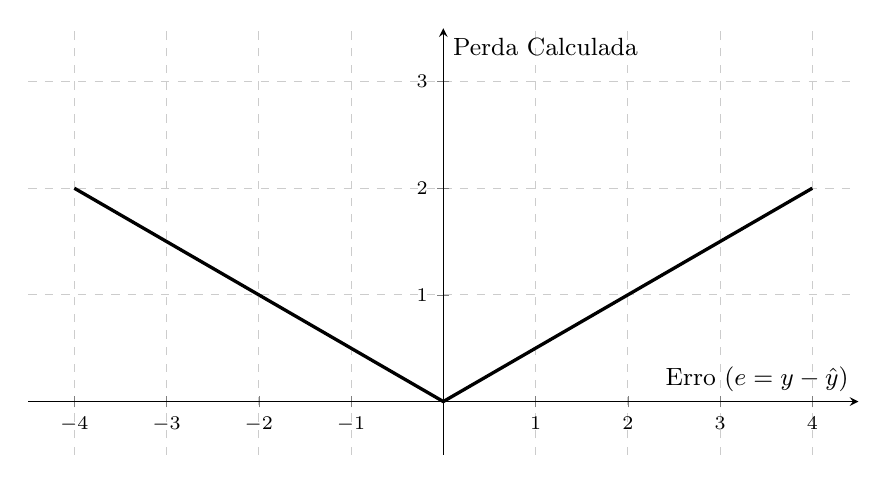
\begin{tikzpicture}
            \begin{axis}[
                width=\linewidth,  
                height=7cm,
                xlabel={Erro ($e = y - \hat{y}$)},
                ylabel={Perda Calculada},
                axis lines=middle,
                grid=major,
                grid style={dashed, gray!40},
                xmin=-4.5, xmax=4.5,
                ymin=-0.5, ymax=3.5,
                legend pos=north west,
                title style={font=\bfseries\small},
                label style={font=\small},
                tick label style={font=\scriptsize},
            ]
                \addplot[domain=-4:4, samples=5, color=black, very thick] {0.5*abs(x)};
            \end{axis}
        \end{tikzpicture}
        \caption{Vista da função de perda em relação ao erro.}%
        \label{fig:quantile-2d-tau05}
    \end{subfigure}
    \hfill 
    \begin{subfigure}[b]{0.48\textwidth}
        \centering
        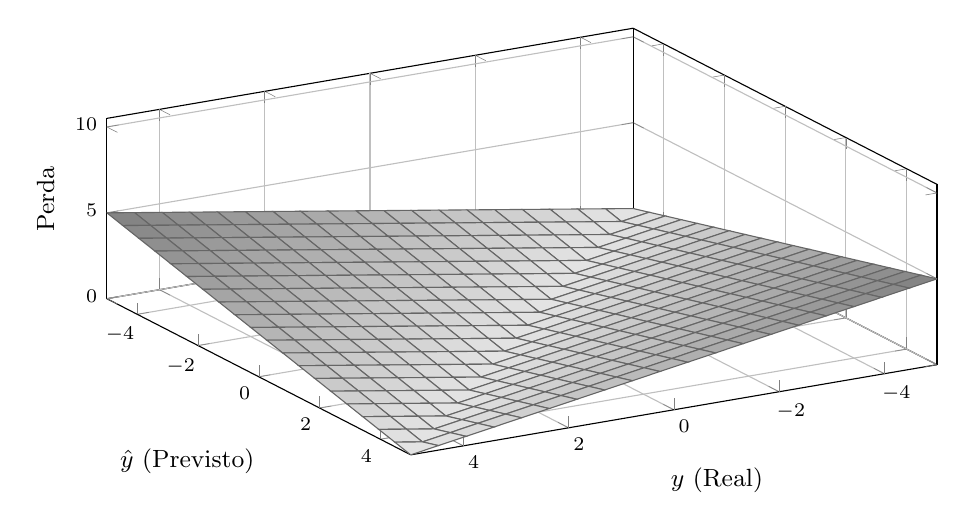
\begin{tikzpicture}
            \begin{axis}[
                width=\linewidth,
                height=7cm,
                xlabel={$y$ (Real)},
                ylabel={$\hat{y}$ (Previsto)},
                zlabel={Perda},
                grid=major,
                view={150}{45},
                zmin=0, zmax=10.5,
                legend pos=north east,
                title style={font=\bfseries\small},
                label style={font=\small},
                tick label style={font=\scriptsize},
                colormap={bw}{gray(0cm)=(0.9); gray(1cm)=(0.5)}
            ]
                \addplot3[
                    surf,           
                    shader=faceted,  
                    faceted color=black!60, 
                    domain=-5:5,    
                    domain y=-5:5, 
                    samples=20,     
                    z buffer=sort
                ] { 0.5*abs(x - y) };
            \end{axis}
        \end{tikzpicture}
        \caption{Superfície da função de perda.}%
        \label{fig:quantile-3d-tau05}
    \end{subfigure}

    \caption{Visualizações da função de perda quantílica em duas e em três dimensões (com $\tau=0.5$ (MAE)).}%
    \label{fig:quantile-loss-tau05}
    \fonte{O autor (2025).}
\end{figure}

O diferencial dessa função é quando ela precisa ser utilizada em cenários em que a distribuição de dados é irregular, e não segue a distribuição normal. Essa função tem a propriedade de se ajustar para penalizar de forma assimétrica os erros que um modelo comete. 

A perda quantílica com hiperparâmetro $\tau = 0,9$, presente na Figura~\ref{fig:quantile-loss-grid}, penaliza fortemente as subestimações feitas pelo modelo. Tem se essa noção inicial devido à sua assimetria, como os gráficos apontam. Quando está sendo analisado o 90º percentil, significa que queremos uma previsão $\hat{y}_j$ que seja maior que 90\% dos valores reais $y_j$. Se o modelo subestima, ou seja $y_j > \hat{y}_j$, ele está falhando o seu objetivo, e terá um erro bem maior.

Um cenário contrário, em que a perda é ajustada para penalizar as superestimações está na Figura~\ref{fig:quantile-loss-grid}. Neste caso, $\tau = 0,1$, ou seja, queremos uma previsão que esteja abaixo dos 10\% dos valores reais. Essa situação é ideal para treinar o modelo a não superestimar os valores, dado que ele será fortemente penalizado se ele fizer uma predição em que $y_j < \hat{y}_j$.

\begin{figure}[h!]
    \centering

    \begin{subfigure}[b]{0.48\textwidth}
        \centering
        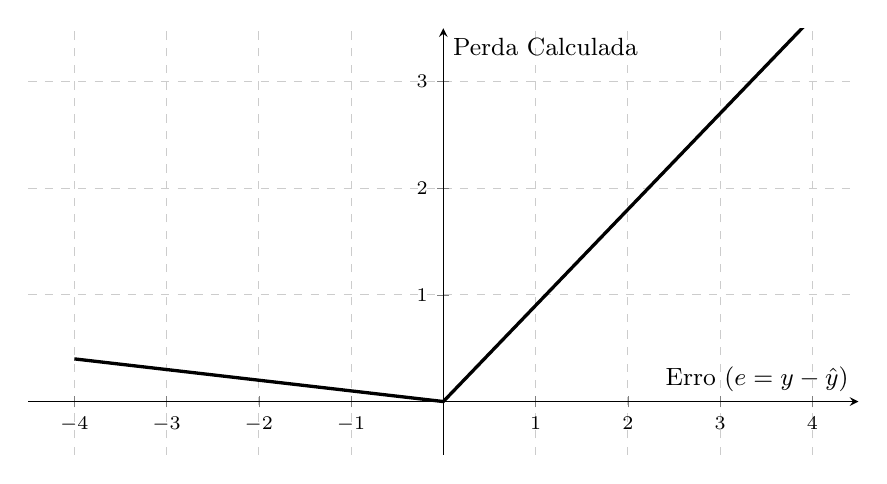
\begin{tikzpicture}
            \begin{axis}[
                width=\linewidth,  
                height=7cm,
                xlabel={Erro ($e = y - \hat{y}$)},
                ylabel={Perda Calculada},
                axis lines=middle,
                grid=major,
                grid style={dashed, gray!40},
                xmin=-4.5, xmax=4.5,
                ymin=-0.5, ymax=3.5,
                legend pos=north west,
                title style={font=\bfseries\small},
                label style={font=\small},
                tick label style={font=\scriptsize},
            ]
                \addplot[domain=-4:4, samples=5, color=black, very thick] {(x >= 0) ? (0.9*x) : ((1-0.9)*(-x))};
            \end{axis}
        \end{tikzpicture}
        \caption{Vista da função de perda em relação ao erro ($\tau=0.9$).}%
        \label{fig:quantile-2d-tau09}
    \end{subfigure}
    \hfill
    \begin{subfigure}[b]{0.48\textwidth}
        \centering
        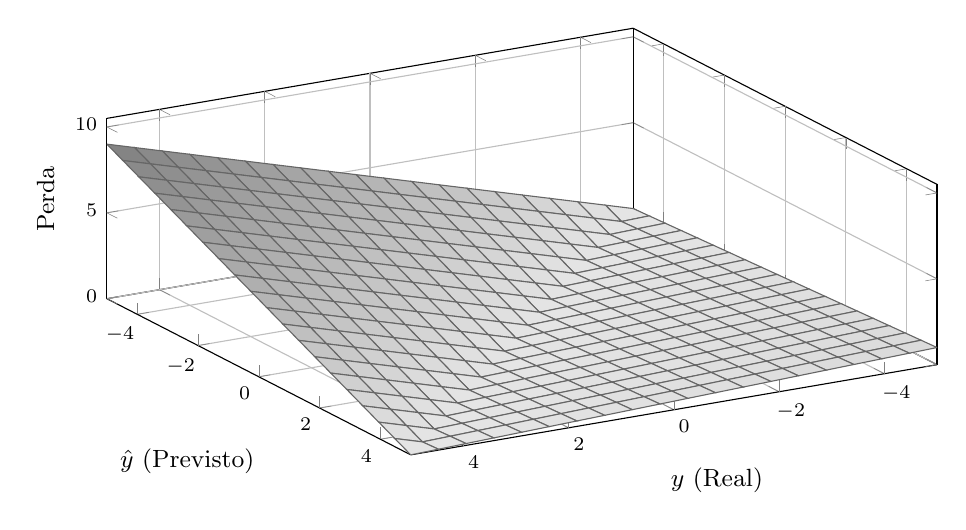
\begin{tikzpicture}
            \begin{axis}[
                width=\linewidth,
                height=7cm,
                xlabel={$y$ (Real)},
                ylabel={$\hat{y}$ (Previsto)},
                zlabel={Perda},
                grid=major,
                view={150}{45},
                zmin=0, zmax=10.5,
                legend pos=north east,
                title style={font=\bfseries\small},
                label style={font=\small},
                tick label style={font=\scriptsize},
                colormap={bw}{gray(0cm)=(0.9); gray(1cm)=(0.5)}
            ]
                \addplot3[
                    surf,           
                    shader=faceted,  
                    faceted color=black!60, 
                    domain=-5:5,    
                    domain y=-5:5, 
                    samples=20,     
                    z buffer=sort
                ] { (x - y >= 0) ? (0.9*(x - y)) : ((1-0.9)*(-(x - y))) };
            \end{axis}
        \end{tikzpicture}
        \caption{Superfície da função de perda ($\tau=0.9$).}%
        \label{fig:quantile-3d-tau09}
    \end{subfigure}

    \vspace{0.5cm} 

    \begin{subfigure}[b]{0.48\textwidth}
        \centering
        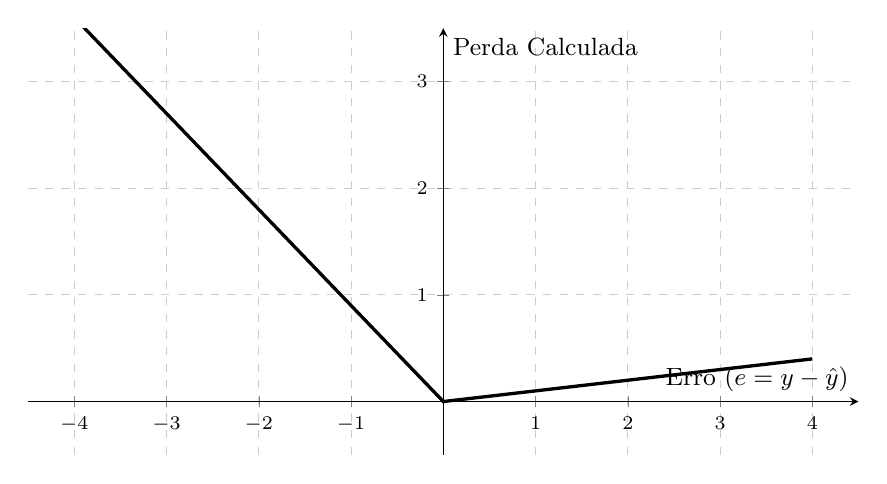
\begin{tikzpicture}
            \begin{axis}[
                width=\linewidth,  
                height=7cm,
                xlabel={Erro ($e = y - \hat{y}$)},
                ylabel={Perda Calculada},
                axis lines=middle,
                grid=major,
                grid style={dashed, gray!40},
                xmin=-4.5, xmax=4.5,
                ymin=-0.5, ymax=3.5,
                legend pos=north west,
                title style={font=\bfseries\small},
                label style={font=\small},
                tick label style={font=\scriptsize},
            ]
                \addplot[domain=-4:4, samples=5, color=black, very thick] {(x >= 0) ? (0.1*x) : ((1-0.1)*(-x))};
            \end{axis}
        \end{tikzpicture}
        \caption{Vista da função de perda em relação ao erro ($\tau=0.1$).}%
        \label{fig:quantile-2d-tau01}
    \end{subfigure}
    \hfill
    \begin{subfigure}[b]{0.48\textwidth}
        \centering
        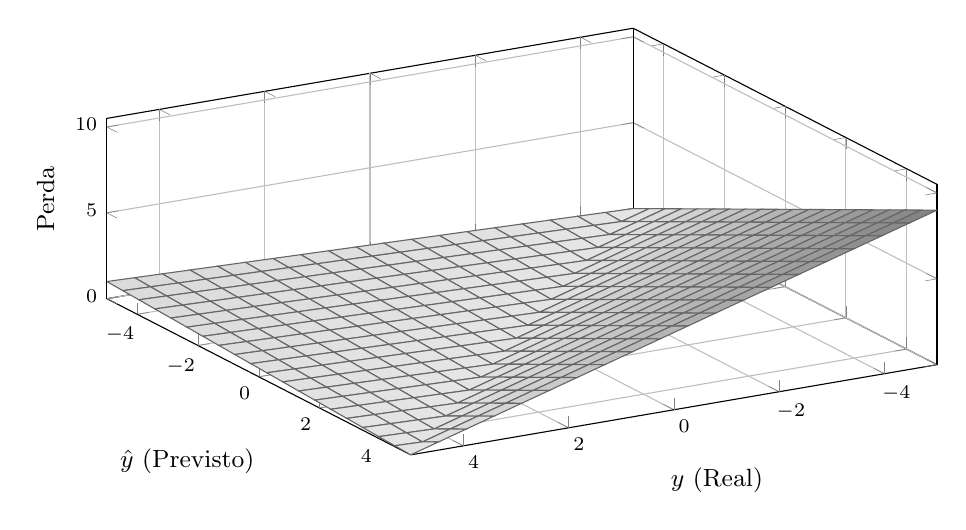
\begin{tikzpicture}
            \begin{axis}[
                width=\linewidth,
                height=7cm,
                xlabel={$y$ (Real)},
                ylabel={$\hat{y}$ (Previsto)},
                zlabel={Perda},
                grid=major,
                view={150}{45},
                zmin=0, zmax=10.5,
                legend pos=north east,
                title style={font=\bfseries\small},
                label style={font=\small},
                tick label style={font=\scriptsize},
                colormap={bw}{gray(0cm)=(0.9); gray(1cm)=(0.5)}
            ]
                \addplot3[
                    surf,           
                    shader=faceted,  
                    faceted color=black!60, 
                    domain=-5:5,    
                    domain y=-5:5, 
                    samples=20,     
                    z buffer=sort 
                ] { (x - y >= 0) ? (0.1*(x - y)) : ((1-0.1)*(-(x - y))) };
            \end{axis}
        \end{tikzpicture}
        \caption{Superfície da função de perda ($\tau=0.1$).}%
        \label{fig:quantile-3d-tau01}
    \end{subfigure}

    \caption{Visualizações das perdas quantílicas para os percentis 90 ($\tau=0.9$) e 10 ($\tau=0.1$).}%
    \label{fig:quantile-loss-grid}
    \fonte{O autor (2025).}
\end{figure}

\subsubsection*{Características da perda quantílica} 

\begin{description}[style=sameline, leftmargin=1.5em, font=\bfseries\color{black}] 
    \item[Continuidade, suavidade e diferenciabilidade:] A perda quantílica é de classe $C^0$, contínua, (ver Apêndice~\ref{ap:deducoes-quantile-loss}). Isso acontece pelo mesmo motivo que o MAE também é de classe $C^0$, essas duas funções apresentam um ``bico'' quando o erro é zero. Como resultado, deve-se analisar os limites laterais dessa função nesse ponto, chegando a conclusão que seus valores divergem. Ainda assim, o uso de subgradiente ajuda a contornar esse problema de suavidade.
    \item[Convexidade:] A perda quantílica é convexa (ver Apêndice~\ref{ap:deducoes-quantile-loss}). Isso é evidenciado também pelos seus gráficos, os quais apontam que essa função apresenta um formato semelhante a um funil. Consequentemente, essa propriedade ajuda os otimizadores baseados em gradiente. Vale destacar que otimizadores baseados em momento vão se comportar diferente conforme forem os valores de $\tau$. Inclinações diferentes podem resultar em otimizações com iterações diferentes.
    \item[Robustez:] A perda quantílica é Lipschitz-contínua, e portanto, robusta a \textit{outliers} (ver Apêndice~\ref{ap:deducoes-quantile-loss}). As suas derivadas parciais quando o erro tende ao infinito são limitadas, garantindo que o gradiente não ``exploda'' quando ocorrem erros grandes.
    \item[Hiperparâmetro $\tau$ (penalização assimétrica):] A perda quantílica é uma função assimétrica, exceto no caso em que $\tau = 0.5$. Como o parâmetro $\tau$ é definido ao treinar ao modelo, cabe a quem estiver treinando o modelo definir se quer que a função penalize mais as subestimações ou as superestimações, a depender do problema que está sendo considerado.
\end{description}

\subsubsection*{Gradiente da perda quantílica}

Para calcular a derivada da perda quantílica, deve-se derivar as duas expressões da Equação~\ref{eq:quantile-loss} e escrever o seu resultado em uma função por partes. Neste caso, está sendo considerado que não existe um valor para o cenário em que a predição é igual ao valor real, ou seja, $\hat{y}_j = y_j$, dado que este é um ponto de descontinuidade dessa função.

Dessa forma, a derivada parcial da perda quantílica em relação à predição feita pelo modelo é dada pela Equação~\ref{eq:quantile-loss-derivada}. Além disso, está sendo indicado os cenários de superestimação e subestimação, de forma a simplificar como os erros do modelo serão corrigidos ao retropropagar o gradiente para as camadas.

\begin{equacaodestaque}{Derivada parcial da perda quantílica em relação à predição}
    \frac{\partial\Loss_{\tau}}{\partial\hat{y}_j} = 
    \begin{cases} 
        (1 - \tau) & \text{se } y_j < \hat{y}_j \text{ (superestimação)}\\
        -\tau & \text{se } y_j > \hat{y}_j \text{ (subestimação)}
    \end{cases}%
    \label{eq:quantile-loss-derivada}
\end{equacaodestaque}

O comportamento da derivada da perda quantílica também se assemelha com MAE. Como a Figura~\ref{fig:quantile-loss-derivada} aponta, a sua derivada é uma função linear por partes, isso ajuda a entender também o porquê da perda quantílica ser robusta a \textit{outliers}. Independente dos valores que o erro pode alcançar, a perda nunca ira crescer descontroladamente para o infinito causando problemas de gradientes explosivos. Diferente do MAE que é 1-Lipschitz-contínua, a perda quantílica tem seus limites modificados conforme o valor do hiperparâmetro $\tau$ é configurado, mas ainda assim, ela é Lipschitz-contínua.

\begin{figure}[h!]
    \centering 

    \begin{subfigure}[b]{0.48\textwidth}
        \centering
        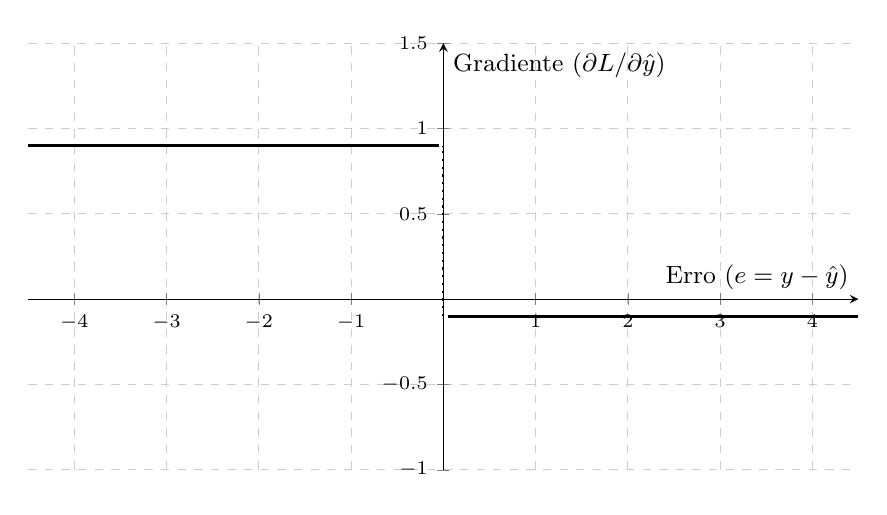
\begin{tikzpicture}
            \begin{axis}[
                width=\linewidth,  
                height=7cm,
                xlabel={Erro ($e = y - \hat{y}$)},
                ylabel={Gradiente ($\partial L / \partial \hat{y}$)},
                axis lines=middle,
                grid=major,
                grid style={dashed, gray!40},
                xmin=-4.5, xmax=4.5,
                ymin=-1.0, ymax=1.5,
                legend pos=north east,
                title style={font=\bfseries\small},
                label style={font=\small},
                tick label style={font=\scriptsize},
                every axis plot post/.append style={mark=none}
            ]
                \addplot[domain=-4.5:-0.05, samples=2, color=black, very thick] {0.9};
                
                \addplot[domain=0.05:4.5, samples=2, color=black, very thick] {-0.1};

                \draw[dotted, thick] (axis cs:0,-0.1) -- (axis cs:0,0.9);
                
            \end{axis}
        \end{tikzpicture}
        \caption{Relação constante por partes entre erro e gradiente da perda.}%
        \label{fig:quantile-deriv-2d-tau01}
    \end{subfigure}
    \hfill 
    \begin{subfigure}[b]{0.48\textwidth}
        \centering
        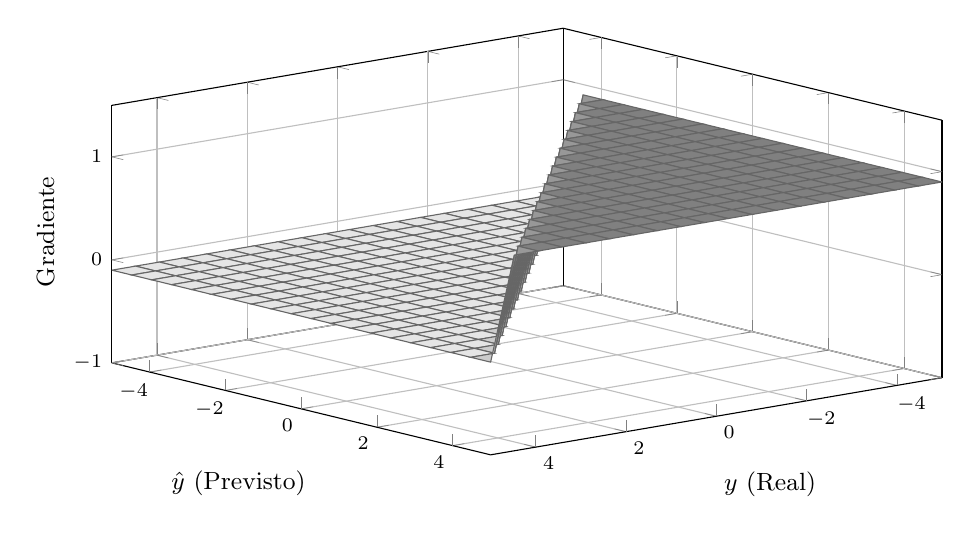
\begin{tikzpicture}
            \begin{axis}[
                width=\linewidth,
                height=7cm,
                xlabel={$y$ (Real)},
                ylabel={$\hat{y}$ (Previsto)},
                zlabel={Gradiente},
                grid=major,
                view={140}{25}, 
                zmin=-1, zmax=1.5,
                title style={font=\bfseries\small},
                label style={font=\small},
                tick label style={font=\scriptsize},
                colormap={bw}{gray(0cm)=(0.9); gray(1cm)=(0.5)}
            ]
                \addplot3[
                    surf,           
                    shader=faceted,  
                    faceted color=black!60, 
                    domain=-5:5,    
                    domain y=-5:5, 
                    samples=20,
                    z buffer=sort
                ] 
                { (x < y) * 0.9 + (x >= y) * (-0.1) };
            \end{axis}
        \end{tikzpicture}
        \caption{Superfície do gradiente no espaço.}%
        \label{fig:quantile-deriv-3d-tau01}
    \end{subfigure}

    \caption{Visualizações do gradiente da perda quantílica em relação à predição (com $\tau = 0.1$).}%
    \label{fig:quantile-loss-derivada}
    \fonte{O autor (2025).}
\end{figure}

\subsubsection*{Aplicações da perda quantílica}%
\index{Aplicações práticas! Perda quantílica}


\begin{description}[style=sameline, leftmargin=1.5em, font=\bfseries\color{black}] 
    \item[Aplicação 1 (Área):] \textcite{candila2023mixedfrequencyquantileregressionsforecast} utilizam a regressão quantílica para prever o VaR (\textit{Value at Risk}) e o \textit{expected shortfall} (ES), para isso, eles criam utilizam de uma técnica diferente, em que é feito o uso de regressões quantílicas de frequência mista. Para fazer isso, os autores combinam dados macroêconomicos de baixa frequência (que são mensais), com dados de mercado de alta frequência (os quais são diários) \parencite{candila2023mixedfrequencyquantileregressionsforecast}.
    \item[Aplicação 2 (Área):] \textcite{Engle2004CAViaR} utilizando a regressão quantílica, apresentam o \textit{Conditional Autoregressive Value at Risk} ou CAVIaR. O CAVIaR propõe uma alternativa diferente para calcular o VaR, ao invés de ser modelado toda a distribuição, com o CAVIaR é calculado apenas o quantil desejado, isso pode ser calculado com o uso da regressão quantílica, e consequentemente com a função de perda quantílica \parencite{Engle2004CAViaR};
    \item[Aplicação 3 (Área):]  \textcite{WINKELMANN2006131} usam a regressão quantílica para contagens para estimar o efeito de uma reforma na saúde sobre a frequência de consultas médicas individuais. O autor justifica a escolha de ser feita uma regressão quantílica, e não uma técnica mais comum, como a dos mínimos quadrados, pois ele considera que esse é um problema em que os efeitos da reforma são diferentes em cada uma das partes da distribuição \parencite{WINKELMANN2006131}.
\end{description}

\medskip

Além da perda quantílica, que é usada nos problemas de regressão quantílica, e que faz o cálculo dos erros considerando uma distribuição irregular dos dados, e por isso não faz o uso da média dos erros para encontrar a perda, existem outras funções que possuem essa mesma característica. Uma dessas funções é a epsilon-insensível, que é essencial para resolver os problemas de regressão para modelos de máquinas de vetores de suporte (SVMs). Ela será explicada em seguida.

\subsection{Perda epsilon-insensível (epsilon-insensitive loss)}%
\index{Funções de Perda!Perda Epsilon-Insensível}

A \textbf{perda epsilon-insensível}, também chamada \textbf{$\epsilon$-insensível} se relacionada diretamente com as máquinas de vetores de suporte, sendo essencial para possibilitar tarefas de regressão pelas SVMs. O trabalho \textit{Support Vector Regression Machines} dos pesquisadores \textcite{SupportVectorRegressionMachines} é um dos responsáveis por introduzir essa função de perda. Nele, os autores detalham um novo uso das máquinas de vetores desenvolvidas por Vapnik, as quais antes eram utilizadas para resolver problemas de classificação \parencite{SupportVectorRegressionMachines}.

\textcite{SupportVectorRegressionMachines} começam o artigo explicando um problema, eles possuem uma função $G(x)$ (chamada de verdade), que recebe um vetor $x$ (chamado de espaço de entradas), esse vetor $x$ possui $d$ componentes, sendo do tipo $x^t = [x_1, x_2, ..., x_d]$. Existe também uma família de funções $F(x, w)$ parametrizadas por $w$ \parencite{SupportVectorRegressionMachines}. O Objeto dos autores é encontrar um parâmetro $\hat{w}$ que é uma estimativa de $w$ a partir de observar um conjunto de $N$ instâncias de treinamento \parencite{SupportVectorRegressionMachines}.

Uma das aproximações para resolver esse problema é a Equação~\ref{eq:svms-para-regressao} como explicam \textcite{SupportVectorRegressionMachines}.

\begin{equation}
    F = (x, \hat{[w]}) = \sum_{i = 1}^N (\alpha_i^*- \alpha_i)(v_i^tx + 1)^p + b
    \label{eq:svms-para-regressao}
\end{equation}

Eles possuem também a função objetiva que querem minimizar, dada pela Equação~\ref{eq:funcao-objetiva-svsms-para-regressao}.

\begin{equation}
    U \sum_{j = 1}^N L [y_j- F(v_j, \hat{w})] + ||\hat{w}||^2
    \label{eq:funcao-objetiva-svsms-para-regressao}
\end{equation}

A função da Equação~\ref{eq:funcao-objetiva-svsms-para-regressao} utiliza uma função de perda, a $\epsilon$-insensível, vista na Equação~\ref{eq:epsilon-insensitive-loss}

\begin{equacaodestaque}{Perda epsilon-insensível}
    \Loss_{\epsilon}(y,\hat{y}) = 
    \begin{cases} 
        0 & \text{se } |y -\hat{y}| < \epsilon\\
        |y -\hat{y}| -\epsilon& \text{se } |y -\hat{y}| \ge\epsilon\end{cases}%
    \label{eq:epsilon-insensitive-loss}
\end{equacaodestaque}

Em que:

\begin{description}[style=sameline, leftmargin=1.5em, font=\bfseries\color{black}]  
    \item[$y_j$] representa o valor real da j-ésima amostra;
    \item[$\hat{y}_j$] representa o valor predito pelo modelo;
    \item[$\epsilon$] representa o tamanho da zona de perda zero.
\end{description}

Como aponta a Figura~\ref{fig:epsilon-insensitive-loss} o seu gráfico lembra um trapézio sem a sua base. Ele possui uma ``zona morta'' de tamanho $\epsilon$, como resultado, se o erro do modelo é menor que o valor absoluto do hiperparâmetro $\epsilon$, o erro não é contabilizado (a função retorna zero). Quando o erro é maior que $\epsilon$ a função calcula a perda de forma linear, assim como o MAE.

\begin{figure}[h!]
    \centering 

    \begin{subfigure}[b]{0.48\textwidth}
        \centering
        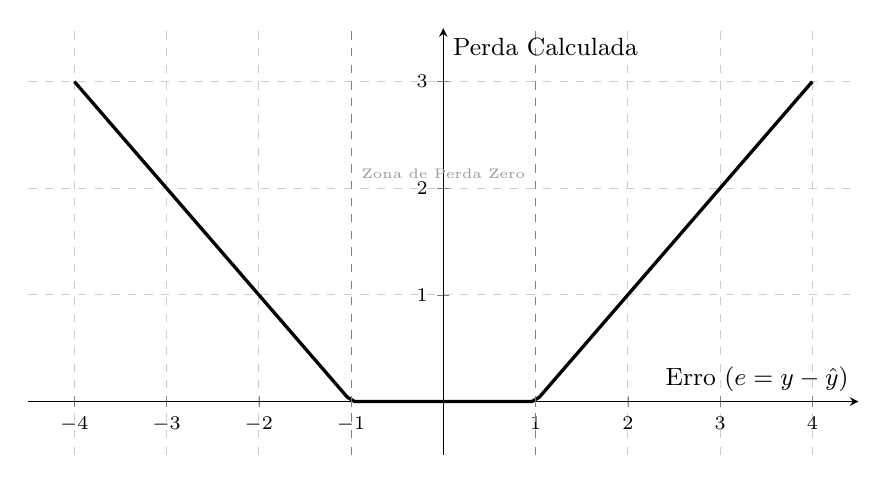
\begin{tikzpicture}
            % Define o valor de epsilon
            \def\epsilon{1.0}
            
            \begin{axis}[
                % Dimensões ajustadas para caber lado a lado
                width=\linewidth,  
                height=7cm,
                xlabel={Erro ($e = y - \hat{y}$)},
                ylabel={Perda Calculada},
                axis lines=middle,
                grid=major,
                grid style={dashed, gray!40},
                xmin=-4.5, xmax=4.5,        % Limites do seu gráfico
                ymin=-0.5, ymax=3.5,         % Limites do seu gráfico
                legend pos=north west,
                title style={font=\bfseries\small},
                label style={font=\small},
                tick label style={font=\scriptsize}
            ]
                % Gráfico da função
                \addplot[
                    domain=-4:4, 
                    samples=101,
                    color=black, 
                    very thick
                ] {max(0, abs(x) - \epsilon)};

                % Linhas tracejadas para marcar a margem epsilon
                \draw[dashed, gray] (axis cs:-\epsilon, -0.5) -- (axis cs:-\epsilon, 3.5);
                \draw[dashed, gray] (axis cs:\epsilon, -0.5) -- (axis cs:\epsilon, 3.5);
                \node[above, gray!80, font=\tiny] at (axis cs:0, 2) {Zona de Perda Zero};
            \end{axis}
        \end{tikzpicture}
        \caption{Vista da função de perda em relação ao erro.}%
        \label{fig:epsilon-2d}
    \end{subfigure}
    \hfill
    \begin{subfigure}[b]{0.48\textwidth}
        \centering
        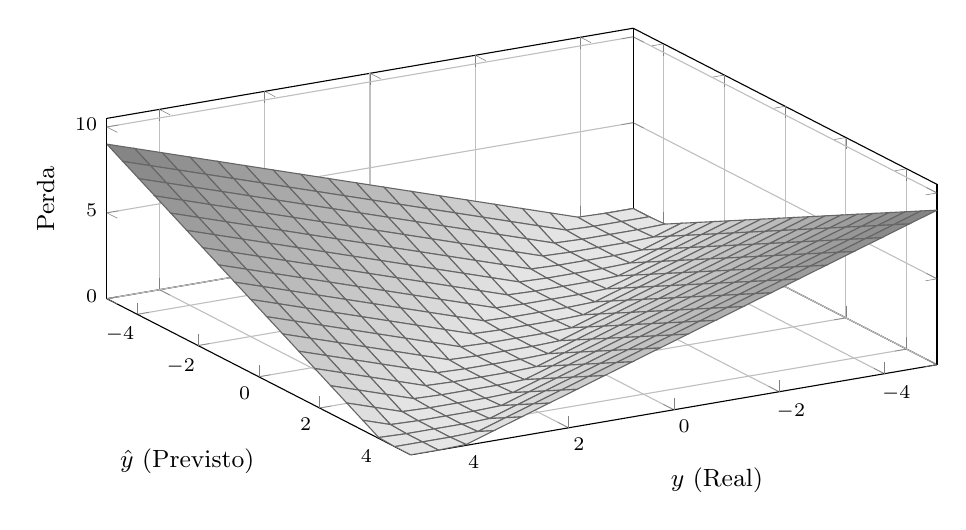
\begin{tikzpicture}
            % Define o valor de epsilon
            \def\epsilon{1.0}
            
            \begin{axis}[
                % Dimensões consistentes com o gráfico (a)
                width=\linewidth,
                height=7cm,
                xlabel={$y$ (Real)},
                ylabel={$\hat{y}$ (Previsto)},
                zlabel={Perda},
                grid=major,
                view={150}{45}, % Mesmo ângulo de visão do seu template
                zmin=0, zmax=10.5, % Ajustado para max(0, abs(10) - 1) = 9
                title style={font=\bfseries\small},
                label style={font=\small},
                tick label style={font=\scriptsize},
                colormap={bw}{gray(0cm)=(0.9); gray(1cm)=(0.5)}
            ]
                \addplot3[
                    surf,           
                    shader=faceted,  
                    faceted color=black!60, 
                    domain=-5:5,    
                    domain y=-5:5, 
                    samples=20,
                    z buffer=sort
                ] { max(0, abs(x - y) - \epsilon) };
            \end{axis}
        \end{tikzpicture}
        \caption{Superfície da função de perda.}%
        \label{fig:epsilon-3d}
    \end{subfigure}

    \caption{Visualizações da função de perda epsilon-insensível (com $\epsilon=1$) em duas e em três dimensões.}%
    \label{fig:epsilon-insensitive-loss}
    \fonte{O autor (2025).}
\end{figure}

Essa região em que o erro é ignorado, é chamada da literatura de Tubo-Epsilon (\textit{$\epsilon$-Tube}). Você pode imaginar um tubo de largura $2\epsilon$, que, qualquer ponto que caia dentro desse tubo não gere penalidade para o modelo.

\subsubsection*{Características da perda epsilon-insensível}

\begin{description}[style=sameline, leftmargin=1.5em, font=\bfseries\color{black}] 
    \item[Continuidade, suavidade e diferenciabilidade:] A perda $\epsilon$-insensível é uma função se classe $C^0$, contínua, (ver Apêndice~\ref{ap:deducoes-epsilon-insensitive}). Isso se dá devido ao fato dessa função não ser suave, ela apresenta dois ``bicos'' que conectam a faixa de ``zona morta'' com o crescimento linear do erro.
    \item[Convexidade:] A perda $\epsilon$-insensível é convexa, embora não estritamente convexa (ver Apêndice~\ref{ap:deducoes-epsilon-insensitive}). A Figura~\ref{fig:epsilon-insensitive-loss} evidencia essa propriedade, a função apresenta um formato de tigela, possuindo uma faixa de pontos de mínimos globais.
    \item[Robustez:] A perda $\epsilon$-insensível é Lipschitz-contínua (ver Apêndice~\ref{ap:deducoes-epsilon-insensitive}). Ao calcular o seu subgradiente, vemos que seu valor é limitado superiormente por 1. Isso garante robustez a \textit{outliers} e ajuda a prevenir problemas de gradientes explosivos.
    \item[Esparsidade:] A perda $\epsilon$-insensível promove a esparsidade no modelo que está sendo treinado. Pelo fato de existir uma faixa de valores do erro que a perda irá retornar zero como valor, essa função de perda ajuda a criar gradientes esparsos nos problemas de regressão de SVMs.
\end{description}

\subsubsection*{Gradiente da perda epsilon-insensível}

Para encontrar o gradiente da perda $\epsilon$-insensível deve-se utilizar do subgradiente, assim como no MAE. O subgradiente consegue lidar com os pontos de não diferenciabilidade (quando erro é igual a epsilon), ao aplicar a técnica chegamos na Equação~\ref{eq:epsilon-insensitive-derivada} para a derivada parcial em relação à predição.

\begin{equacaodestaque}{Derivada parcial da perda epsilon-insensível em relação à predição}
    \frac{\partial\Loss_{\epsilon}}{\partial\hat{y}} = 
    \begin{cases} 
        1 & \text{se } \hat{y} -y > \epsilon\\
        0 & \text{se } |\hat{y} -y| \le\epsilon\\
        -1 & \text{se } \hat{y} -y < -\epsilon\end{cases}%
    \label{eq:epsilon-insensitive-derivada}
\end{equacaodestaque}

Os gráficos da derivada parcial da $\epsilon$-insensível ajudam a evidenciar as suas propriedades de esparsidade de robustez. Como a Figura~\ref{fig:epsilon-derivada-completa} mostra, essa função retorna zero para um conjunto de valores do gradiente, além de não existir nenhum ponto em que ela ultrapasse o valor de 1. Apenas os pontos que caem fora do tubo (onde o gradiente $\pm 1$) se tornam os chamados vetores de suporte. Como o modelo é esparso, ele ignora os dados fáceis (de erro pequeno, e que caem dentro do tubo), e foca apenas nos difíceis, os vetores de suporte.


\begin{figure}[h!]
    \centering
    \def\epsilon{1.0}
    \def\yreal{5.0}

    \begin{subfigure}[b]{0.48\textwidth}
        \centering
        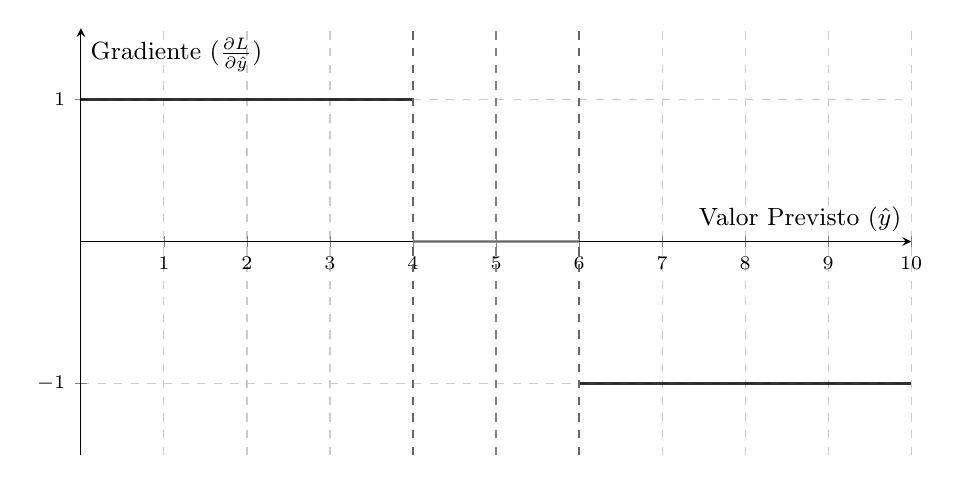
\begin{tikzpicture}
            \begin{axis}[
                width=\linewidth,  
                height=7cm,
                xlabel={Valor Previsto ($\hat{y}$)},
                ylabel={Gradiente ($\frac{\partial L}{\partial \hat{y}}$)},
                axis lines=middle,
                grid=major,
                grid style={dashed, gray!40},
                xmin=0, xmax=10,
                ymin=-1.5, ymax=1.5,
                ytick={-1, 0, 1},
                legend pos=north west,
                title style={font=\bfseries\small},
                label style={font=\small},
                tick label style={font=\scriptsize}
            ]
                
                \addplot[const plot, color=black, very thick, opacity=0.8] 
                    coordinates { (0, 1) (\yreal - \epsilon, 1) };
                
                \addplot[const plot, color=gray, very thick, opacity=0.8] 
                    coordinates { (\yreal - \epsilon, 0) (\yreal + \epsilon, 0) };
                
                \addplot[const plot, color=black, very thick, opacity=0.8] 
                    coordinates { (\yreal + \epsilon, -1) (10, -1) };

                \draw[dashed, gray] (axis cs:\yreal, -1.5) -- (axis cs:\yreal, 1.5);
                \node[above, gray!80, font=\tiny] at (axis cs:\yreal, 1.5) {Valor Real};
                
                \draw[dashed, black!60] (axis cs:\yreal-\epsilon, -1.5) -- (axis cs:\yreal-\epsilon, 1.5);
                \draw[dashed, black!60] (axis cs:\yreal+\epsilon, -1.5) -- (axis cs:\yreal+\epsilon, 1.5);

            \end{axis}
        \end{tikzpicture}
        \caption{Relação constante por partes entre erro e gradiente da perda.}%
        \label{fig:epsilon-derivada-2d}
    \end{subfigure}
    \hfill 
    \begin{subfigure}[b]{0.48\textwidth}
        \centering
        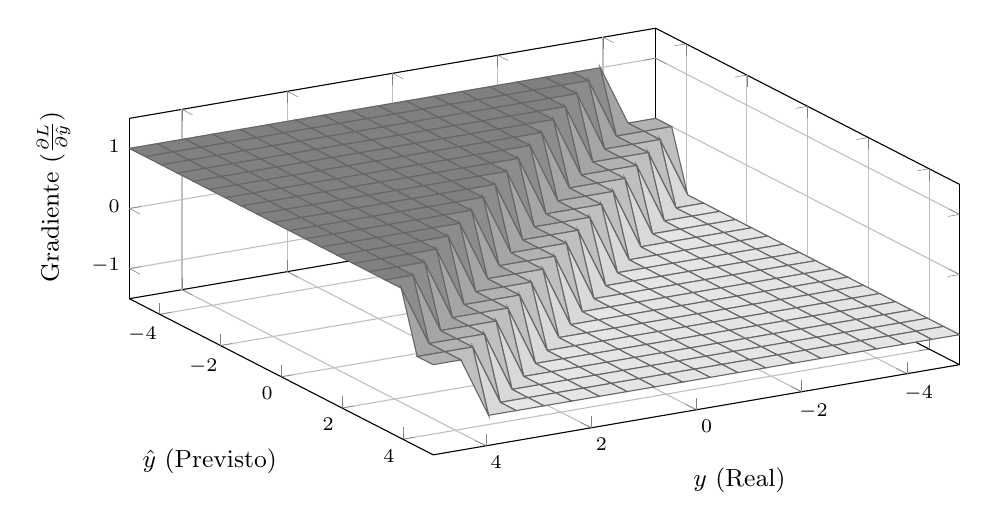
\begin{tikzpicture}
            \begin{axis}[
                width=\linewidth,
                height=7cm,
                xlabel={$y$ (Real)},
                ylabel={$\hat{y}$ (Previsto)},
                zlabel={Gradiente ($\frac{\partial L}{\partial \hat{y}}$)},
                grid=major,
                view={150}{45}, % Mesmo ângulo de visão do seu template
                zmin=-1.5, zmax=1.5,
                ztick={-1, 0, 1}, % Ticks exatos da derivada
                title style={font=\bfseries\small},
                label style={font=\small},
                tick label style={font=\scriptsize},
                colormap={bw}{gray(0cm)=(0.9); gray(1cm)=(0.5)}
            ]
                \addplot3[
                    surf,           
                    shader=faceted,  
                    faceted color=black!60, 
                    domain=-5:5,    
                    domain y=-5:5, 
                    samples=20,
                    z buffer=sort
                ] { (y - x > \epsilon) ? -1 : ( (y - x < -\epsilon) ? 1 : 0 ) }; 
            \end{axis}
        \end{tikzpicture}
        \caption{Superfície do gradiente no espaço.}%
        \label{fig:epsilon-derivada-3d}
    \end{subfigure}

    \caption{Visualizações do gradiente da perda $\epsilon$-insensível em relação à predição (com $\epsilon = 1$).}%
    \label{fig:epsilon-derivada-completa}
    \fonte{O autor (2025).}
\end{figure}

\subsubsection*{Aplicações da perda epsilon-insensível}%
\index{Aplicações práticas! Perda epsilon-insensível}

\begin{description}[style=sameline, leftmargin=1.5em, font=\bfseries\color{black}] 
    \item[Aplicação 1 (Área):] 
    \item[Aplicação 2 (Área):] 
    \item[Aplicação 3 (Área):] 
\end{description}

\section{Perdas baseadas em distribuições de dados}%
\label{sec:perdas-baseadas-em-distribuicoes-de-dados}

Exceto pela perda $\epsilon$-insensível que trabalha com distribuições que não eram simétricas, a maioria das perdas apresentadas até agora são utilizadas para dados que seguem a distribuição Normal. Isso foi visto na explicação sobre o erro quadrático médio, e como Gauss prova que o método dos mínimos quadrados é uma solução ideal para ser utilizado em casos em que os dados seguem a distribuição Gaussiana.

Contudo, mesmo a distribuição normal sendo a mais comum para modelar os diferentes problemas que envolvem regressão, existem outras distribuições que são igualmente importantes. Essa seção foca em explicar três funções de perda que são utilizadas para trabalhar com distribuições específicas, são elas: a perda de Poisson, a perda Gamma e a perda de Tweedie.

\subsection{Perda de Poisson (Poisson loss)}%
\index{Funções de Perda!Perda de Poisson (\textit{Poisson loss})}

Imagine que você está procurando uma forma de modelar a quantidade de ligações que você pode receber em seu telefone por dia. Primeiro, você pensou que essa quantidade seguiria uma distribuição normal, mas encontrou um problema, a distribuição normal é contínua, e não tem como você receber $2,5$ ligações em um período. Além disso, você decidiu que precisava dividir o tempo em um conjunto de intervalos discretos, assim, todas as ligações que você receber das 14:00 as 14:59 ficarão no mesmo intervalo. Esse problema possui ainda uma terceira particularidade, não existe um limite de ligações que você pode receber, pode ser que das 13:00 as 13:59 você receba duas ligações, mas também pode ser que você receba 314 ligações naquele horário. Quando temos uma situação parecida com essa, nós estaremos trabalhando com o que os estatísticos chamam de \textbf{dados de contagem}. 

Nessas situações, a distribuição normal não irá ser efetiva, sendo necessárias distribuições como a de Poisson.

\subsubsection*{A distribuição de Poisson}%
\index{Distribuição de Poisson}

A função densidade de probabilidade da distribuição de Poisson é dada pela Equação~\ref{eq:poisson-distribution-pmf}, onde o espaço amostral é conjunto de inteiros não-negativos. Em \textit{Generalized Linear Models}, \textcite{GeneralizedLinearModels} aponta que essa distribuição não possui uma limite superior nos valores que podem ser observados, diferente da distribuição Normal.

\begin{equacaodestaque}{Distribuição de Poisson (FMP)}
    P(y_j| \lambda) = \frac{\lambda^{y_j} e^{-\lambda}}{y_j!}, \quad y_j \in {0, 1, 2, \ldots}%
    \label{eq:poisson-distribution-pmf}
\end{equacaodestaque}

Em que

\begin{itemize}
    \item $\lambda$ representa a taxa de Poisson, ou seja, a contagem esperada.
\end{itemize}

A distribuição de Poisson segue a média, a variância e todos os cumulativos de $Y$ que são iguais a $\lambda$ \parencite{GeneralizedLinearModels}. Isso significa que a média e a variância dessa distribuição são iguais, consequentemente, o parâmetro $\lambda$ é o único responsável por controlar como a distribuição se comporta. Considerando a distribuição normal, que precisa de dois parâmetros ($\mu$ para a média e $\sigma^2$ para a variância), na Poisson o parâmetro $\lambda$ é quem dita a tendência central, onde os dados se agrupam, e também a dispersão, indicando se eles estão muito ou pouco espalhados.

Quando utilizamos o MSE como função de perda, estamos supondo que os dados seguem a distribuição normal, e portanto a variância é constante em toda a distribuição. Se fazemos uso dessa função de perda para um cenário em que temos dados de contagem que seguem a distribuição de Poisson, o MSE irá penalizar excessivamente os erros em contagem alta (na qual o ruído é maior) e insuficientemente em contagem baixa. A perda de Poisson consegue corrigir esse problema, dado que ela leva em consideração a definição da função log-verossimilhança da distribuição de Poisson.

Na Figura~\ref{fig:poisson-low-lambda} o parâmetro $\lambda$ é igual a 1, ele é baixo. Portanto, a média da distribuição é baixa, de forma que a maioria dos dados está próxima de zero. A variância também é baixa, indicando que os dados são representados no gráfico de forma assimétrica. Já na Figura~\ref{fig:poisson-high-lambda} o cenário é o inverso, o $\lambda$ é alto. Com isso, os dados ficam melhores distribuídos no gráfico, além de uma média maior. O gráfico passa a lembrar o de uma distribuição Normal, mas ainda assim, permanece discreto. Além disso, o parâmetro $\lambda$ é responsável por definir também a assimetria dos gráficos da distribuição, conforme seu valor aumenta, a assimetria diminui.

\begin{figure}[h!]
    \centering 

    \begin{subfigure}[b]{0.48\textwidth}
        \centering
        \begin{tikzpicture}
            \begin{axis}[
              axis x line=center,
              axis y line=center,
              xtick={0,2,...,19},
              ytick={0.1,0.2,...,0.4},
                domain = 0:18,
                samples = 19,
                xlabel={$k$},
                ylabel={$P[k]$},
                xlabel style={right},
                ylabel style={above left},
                ymax=0.5,
                xmax=20,
                x post scale=1.4
                ]
                \addplot[ycomb,black,thick] {poisson(1)};
                \addlegendentry{$\lambda = 1$}
            \end{axis}
        \end{tikzpicture}
        \caption{Com $\lambda$ baixo, a distribuição é assimétrica e ``espremida'' perto do zero.}%
        \label{fig:poisson-low-lambda}
    \end{subfigure}
    \hfill
    
    \begin{subfigure}[b]{0.48\textwidth}
        \centering
        \begin{tikzpicture}
            \begin{axis}[
              axis x line=center,
              axis y line=center,
              xtick={0,2,...,19},
              ytick={0.1,0.2,...,0.4},
                domain = 0:18,
                samples = 19,
                xlabel={$k$},
                ylabel={$P[k]$},
                xlabel style={right},
                ylabel style={above left},
                ymax=0.5,
                xmax=20,
                x post scale=1.4
                ]
                \addplot[ycomb,black,thick] {poisson(9)};
                 \addlegendentry{$\lambda = 9$};
            \end{axis}
        \end{tikzpicture}

        \caption{Com $\lambda$ alto, a distribuição se aproxima de uma curva Normal (Gaussiana), mas permanece discreta.}%
        \label{fig:poisson-high-lambda}
    \end{subfigure}
    
    \caption{Comparação visual da Distribuição de Poisson com $\lambda$ baixo e alto.}
    \label{fig:poisson-comparison}
    \fonte{O autor (2025).}
\end{figure}

Ainda em \textit{Generalized Linear Models}, \textcite{GeneralizedLinearModels} explicam algum cenários em que essa distribuição é utilizada para descrever um problema, entre algum dos explicados pelo autor, vale a pena citar:

\begin{itemize}
    \item \textbf{Um ensaio biológico sobre tuberculina:} A distribuição de poisson com a sua função de log-verossimilhança é utilizada para descrever os casos de tuberculina em população de bovinos;
    \item \textbf{Um estudo sobre o dano das ondas em navios cargueiros:} xxx utilizam a distribuição de poisson assim como o cálculo da log-verossimilhança para estimar o dano das ondas em navios cargueiros.
\end{itemize}

Na prática um bom indicativo para considerar utilizar a distribuição de poisson e a perda de Poisson, é considerar as próprias características dessa distribuição. Ao analisar um problema e perceber que os dados seguem uma distribuição discreta, são inteiros não negativos e que a média dos dados é igual a variância, talvez valha a pena ver se a distribuição de Poisson pode ser aplicada.

\medskip

\subsubsection*{Perda de Poisson}

Para chegar na definição da perda de Poisson, devemos começar com função log-verossimilhança da distribuição. Ela é dada por

A função log-verossimilhança para a distribuição de Poisson está na Equação~\ref{eq:log-verossimilhanca-negativa-de-poisson}, é a partir dela que chegaremos na definição da perda de Poisson.

\[
    \log (P(y_j|\lambda)) =  -\lambda + y_j \log(\lambda_j) - \log(y_j!)
\]

O termo $\log(y_j !)$ é constante em relação ao modelo, dado que o modelo não controla o valor real $y_j$, só a previsão $\lambda$. Então escrevemos

\[
      -\lambda + y_j \log(\lambda_j)
\]

Como nosso intuito é minimizar a perda, devemos multiplicá-la por $-1$. Feito isso, encontramos que a perda de Poisson é dada pela Equação~\ref{eq:poisson-loss}. Neste caso, o termo $\lambda_j$ é dado pelo valor predito pelo modelo $\hat{y}_j$.

\begin{equacaodestaque}{Perda de Poisson}
    \Loss_{\text{Poisson}}(y_j, \hat{y}_j) = \sum_{j = 0}^N \hat{y}_j -y_j \log(\hat{y}_j)%
    \label{eq:poisson-loss}
\end{equacaodestaque}

Em que:

\begin{description}[style=sameline, leftmargin=1.5em, font=\bfseries\color{black}]  
    \item[$y_j$] representa o valor real da j-ésima amostra;
    \item[$\hat{y}_j$] representa o valor predito pelo modelo;
    \item[$N$] representa o número de amostras.
\end{description}

Como o valor real $y_j$ não é controlado pelo modelo, conforme ele for variando de iteração para iteração, vão existir diferentes gráficos de perda, isso está evidenciado na Figura~\ref{fig:poisson-comparison}. Quando o valor real é pequeno, a perda de Poisson possui uma convexidade mais ``apertada''. Já quando o valor real é grande, isso resulta em uma função mais ``larga''.

\begin{figure}[h!]
    \centering

    \begin{subfigure}[b]{0.48\textwidth}
        \centering
        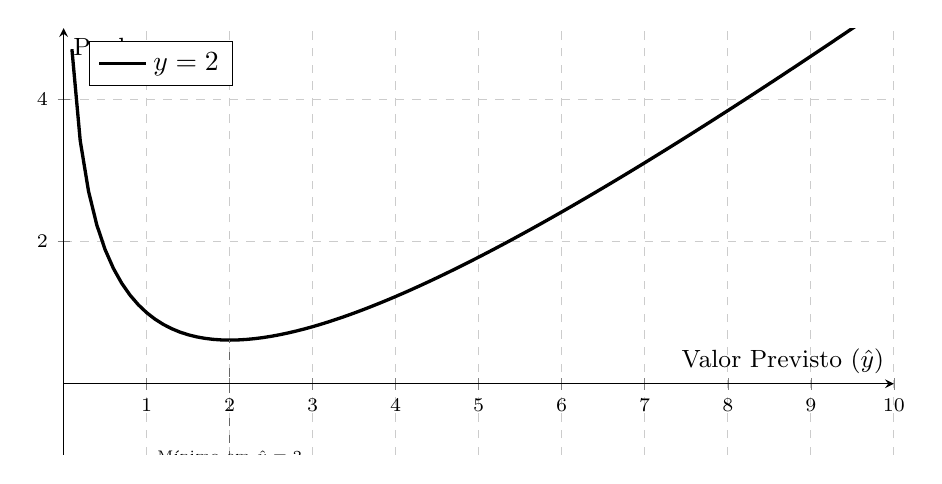
\begin{tikzpicture}
            \begin{axis}[
                width=\linewidth,  
                height=7cm,
                xlabel={Valor Previsto ($\hat{y}$)},
                ylabel={Perda},
                axis lines=middle,
                grid=major,
                grid style={dashed, gray!40},
                xmin=0, xmax=10,
                ymin=-1, ymax=5,
                legend pos=north west,
                title style={font=\bfseries\small},
                label style={font=\small},
                tick label style={font=\scriptsize},
            ]
                % Perda Poisson: x - y*ln(x) -> Aqui x é y_hat, y fixo em 2
                \addplot[domain=0.1:10, samples=100, color=black, very thick] {x - 2*ln(x)};
                \addlegendentry{$y=2$}
                
                % Linha pontilhada no mínimo
                \draw[dashed, black!60] (axis cs:2, -2) -- (axis cs:2, {2-2*ln(2)});
                \node[anchor=north, font=\tiny, text=black] at (axis cs:2, -0.8) {Mínimo em $\hat{y}=2$};
            \end{axis}
        \end{tikzpicture}
        \caption{Comportamento para valor real baixo.}%
        \label{fig:poisson-2d-low}
    \end{subfigure}
    \hfill
    \begin{subfigure}[b]{0.48\textwidth}
        \centering
        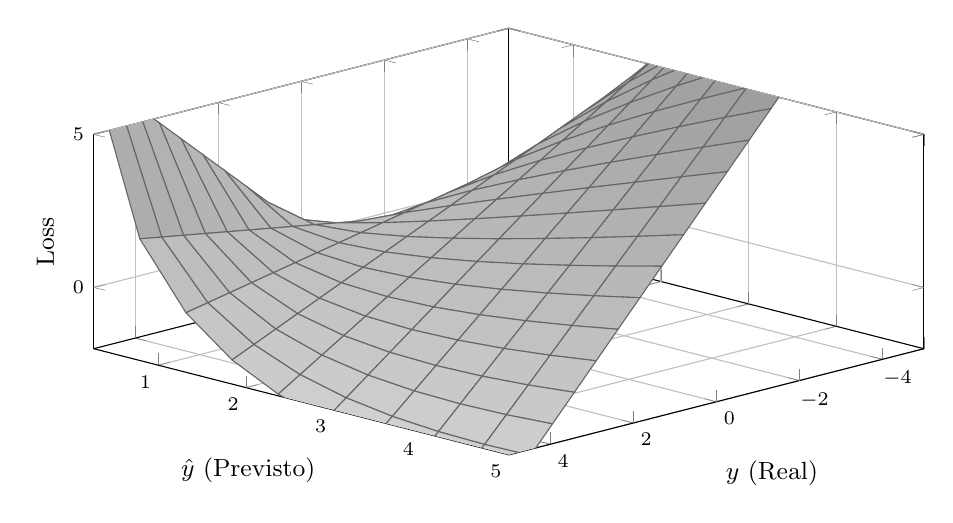
\begin{tikzpicture}
            \begin{axis}[
                width=\linewidth,
                height=7cm,
                xlabel={$y$ (Real)},
                ylabel={$\hat{y}$ (Previsto)},
                zlabel={Loss},
                grid=major,
                view={135}{35}, % Angulo de visão
                legend pos=north east,
                title style={font=\bfseries\small},
                label style={font=\small},
                tick label style={font=\scriptsize},
                zmin=-2, zmax=5,
                colormap={bw}{gray(0cm)=(0.9); gray(1cm)=(0.5)}
            ]
                \addplot3[
                   surf,           
                    shader=faceted,  
                    faceted color=black!60, 
                    domain=-5:5,    
                    domain y=-5:5, 
                    samples=20,
                    z buffer=sort
                ] { y - x*ln(y) };
            \end{axis}
        \end{tikzpicture}
        \caption{Superfície local (Região $1 \le y \le 5$).}%
        \label{fig:poisson-3d-low}
    \end{subfigure}

    \vspace{0.5cm} 

    \begin{subfigure}[b]{0.48\textwidth}
        \centering
        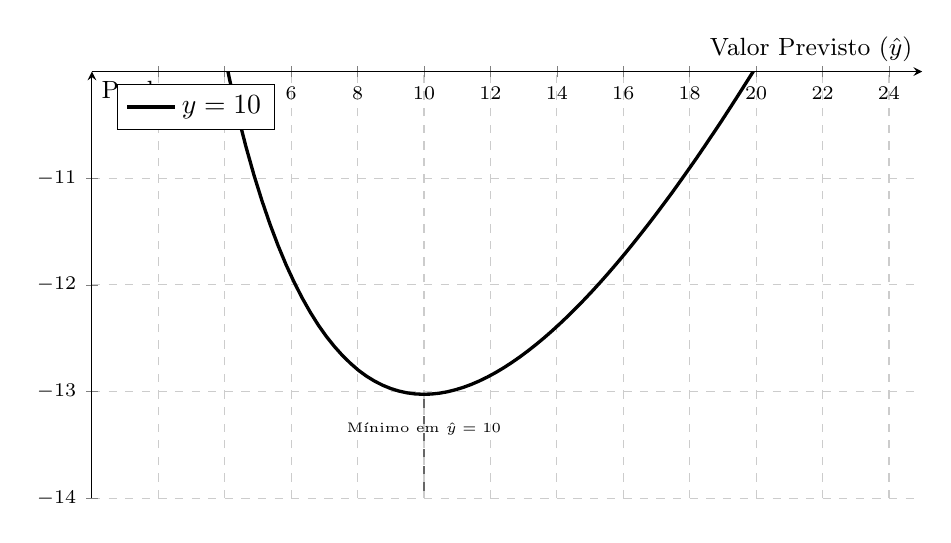
\begin{tikzpicture}
            \begin{axis}[
                width=\linewidth,  
                height=7cm,
                xlabel={Valor Previsto ($\hat{y}$)},
                ylabel={Perda},
                axis lines=middle,
                grid=major,
                grid style={dashed, gray!40},
                xmin=0, xmax=25,
                % Ajustando ymin/ymax para focar na curvatura
                ymin=-14, ymax=-10, 
                legend pos=north west,
                title style={font=\bfseries\small},
                label style={font=\small},
                tick label style={font=\scriptsize},
            ]
                % Perda Poisson para y=10
                \addplot[domain=1:25, samples=100, color=black, very thick] {x - 10*ln(x)};
                \addlegendentry{$y=10$}
                
                % Linha pontilhada no mínimo
                \draw[dashed, black!60] (axis cs:10, -20) -- (axis cs:10, {10-10*ln(10)});
                 \node[anchor=north, font=\tiny, text=black] at (axis cs:10, -13.2) {Mínimo em $\hat{y}=10$};
            \end{axis}
        \end{tikzpicture}
        \caption{Comportamento para valor real alto.}%
        \label{fig:poisson-2d-high}
    \end{subfigure}
    \hfill
    \begin{subfigure}[b]{0.48\textwidth}
        \centering
        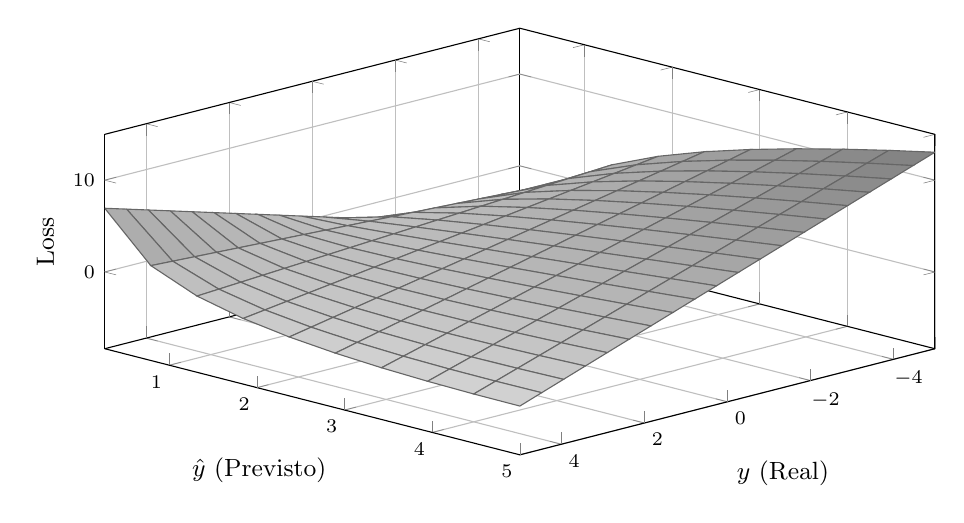
\begin{tikzpicture}
            \begin{axis}[
                width=\linewidth,
                height=7cm,
                xlabel={$y$ (Real)},
                ylabel={$\hat{y}$ (Previsto)},
                zlabel={Loss},
                grid=major,
                view={135}{35},
                title style={font=\bfseries\small},
                label style={font=\small},
                tick label style={font=\scriptsize},
                colormap={bw}{gray(0cm)=(0.9); gray(1cm)=(0.5)}
            ]
                % Formula: y - x * ln(y) (x=Real, y=Previsto)
                \addplot3[
                   surf,           
                    shader=faceted,  
                    faceted color=black!60, 
                    domain=-5:5,    
                    domain y=-5:5, 
                    samples=20,
                    z buffer=sort
                ] { y - x*ln(y) };
            \end{axis}
        \end{tikzpicture}
        \caption{Superfície local (Região $8 \le y \le 12$).}%
        \label{fig:poisson-3d-high}
    \end{subfigure}

    \caption{Comparação da perda de Poisson para diferentes magnitudes de $y$.}%
    \label{fig:poisson-loss-grid}
    \fonte{O autor (2025).}
\end{figure}

\subsubsection*{Características da perda de Poisson}

\begin{description}[style=sameline, leftmargin=1.5em, font=\bfseries\color{black}] 
    \item[Continuidade, suavidade e diferenciabilidade:] A perda de Poisson pertence à classe $C^\infty$ (infinitamente diferenciável) em seu domínio de definição $(0, \infty)$ (ver Apêndice~\ref{ap:deducoes-poisson-loss}). Isso garante para essa função a possibilidade de ser utilizada tanto em métodos de otimização baseados em gradiente (que utilizam a primeira derivada) quanto em métodos de segunda ordem (que utilizam a segunda derivada).
    \item[Convexidade:] A perda de Poisson é convexa, e estritamente convexa se $y > 0$ (ver Apêndice~\ref{ap:deducoes-poisson-loss}). Esse fato está evidenciado nos gráficos da Figura~\ref{fig:poisson-comparison}, independentemente dos valores reais $y_j$, a perda segue um comportamento de uma função convexa, com o gráfico semelhante a um ``funil''.
    \item[Robustez:] A perda de Poisson não é Lipschitz-contínua globalmente devido à singularidade na origem (ver Apêndice~\ref{ap:deducoes-poisson-loss}). Para uma função ser Lipschitz-contínua, o seu gradiente deve ser limitado, algo que não acontece quando a predição aproxima de zero. Desse modo, ao utilizar essa função de perda, tenha em mente que o modelo criado estará susceptível a gradientes explosivos.
    \item[Não-negatividade e funções de conexão:] Ao definir a perda de Poisson é utilizado o logaritmo, isso implica que o termo $\log(\hat{y}_j)$ deve ser sempre positivo. Esse fato também é exposto ao definir a própria distribuição de Poisson, os dados de contagem não devem ser negativos. Em modelos lineares generalizados a função exponencial é comumente utilizada como uma função de conexão (\textit{link function}) para garantir que esses valores se encaixem nesse intervalo \parencite{LossesArticle}. Assim, cabe discutir uma definição alternativa para a perda de Poisson, em que consideramos a exponencial como uma função de conexão:

    Sabemos que um modelo de aprendizado de máquina, geralmente retorna algo que segue o padrão
 
    \[
        \hat{y}_j = \textbf{W}^T x_j + b
    \]

    Esse valor pode ser negativo e queremos que ele fique em um intervalo $\hat{y} > 0$. Uma das soluções é utilizar a função exponencial como uma função de conexão, então escrevemos

    \[
        \hat{y}_j = \text{exp}(\textbf{W}^T x_j + b)
    \]

    Ao substituir essa expressão na Equação~\ref{eq:poisson-loss} chegamos nos termos

    \[
        \Loss_{\text{Poisson}}(y_j, \hat{y}_j) = \sum_{j = 0}^N \text{exp}(\textbf{W}^T x_j + b) - y_j \log(\text{exp}(\textbf{W}^T x_j + b))
    \]

    Simplificando os cálculos do logaritmo, encontramos

    \[
        \Loss_{\text{Poisson}}(y_j, \hat{y}_j) = \sum_{j = 0}^N \text{exp}(\textbf{W}^T x_j + b) - y_j  (\text{exp}(\textbf{W}^T x_j + b))
    \]

    Que pode ser reescrita uma última vez como 

    \[
        \Loss_{\text{Poisson}}(y_j, \hat{y}_j) = \sum_{j = 0}^N \text{exp}(\hat{y}_j) - y_j  (\text{exp}(\hat{y}_j))
    \]
\end{description}

\subsubsection*{Gradiente da perda de Poisson}

A derivada parcial da perda de Poisson em relação à predição $\hat{y}_j$ feita pelo modelo está representada na Equação~\ref{eq:poisson-loss-derivada}.

\begin{equacaodestaque}{Derivada parcial da perda de Poisson em relação à predição}
    \frac{\partial\Loss_{\text{Poisson}}}{\partial\hat{y}_j} = 1 -\frac{y_j}{\hat{y}_j} = \frac{\hat{y}_j -y_j}{\hat{y}_j}%
    \label{eq:poisson-loss-derivada}
\end{equacaodestaque}

Conforme os valores reais $y_j$ variam, a curva do gráfico da derivada da perda de Poisson também varia. A Figura~\ref{fig:poisson-loss-derivada} aponta que quanto maior é o valor de $y_j$ mais próximo do eixo das abscissas fica a curva da perda. Dessa forma, o gradiente é zero quando $\hat{y}_j = y_j$ e é assintótico quando $\hat{y}_j \to \infty$.

\begin{figure}[h!]
    \centering
    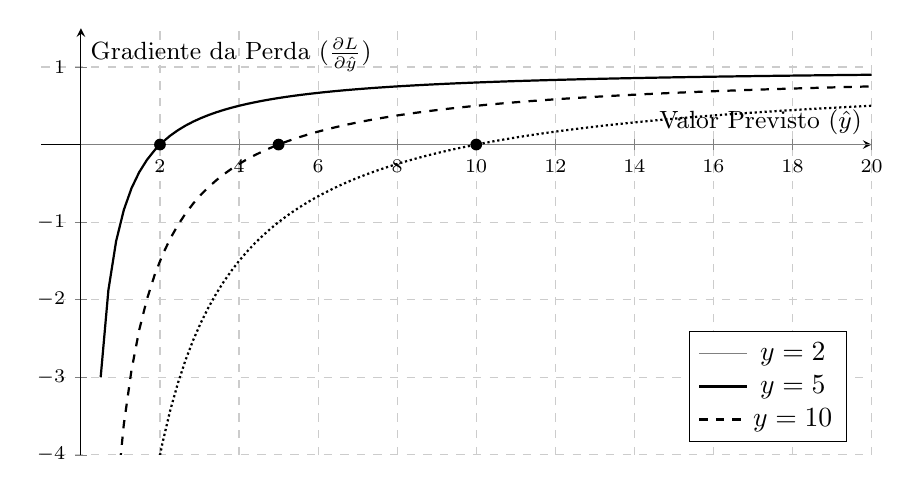
\begin{tikzpicture}
        \begin{axis}[
            xlabel={Valor Previsto ($\hat{y}$)},
            ylabel={Gradiente da Perda ($\frac{\partial L}{\partial \hat{y}}$)},
            axis lines=middle,
            grid=major,
            grid style={dashed, gray!40},
            xmin=-1, xmax=20,
            ymin=-4, ymax=1.5,
            legend pos=south east,
            width=\linewidth,
            height=7cm,
            title style={font=\bfseries},
            label style={font=\small},
            tick label style={font=\scriptsize}
        ]

            % Linha de referência (Zero) - Opcional, mas ajuda visualmente
            \addplot[gray, thin] coordinates {(0,0) (20,0)};

            % Curva para y=2 (Linha Sólida)
            \addplot[domain=0.5:20, samples=101, color=black, thick] {1 - 2/x};
            \addlegendentry{$y=2$}
            
            % Curva para y=5 (Linha Tracejada Longa)
            \addplot[domain=0.5:20, samples=101, color=black, thick, dashed] {1 - 5/x};
            \addlegendentry{$y=5$}

            % Curva para y=10 (Linha Pontilhada/Densa)
            \addplot[domain=0.5:20, samples=101, color=black, thick, densely dotted] {1 - 10/x};
            \addlegendentry{$y=10$}
            
            % Adicionei nós (nodes) para destacar onde o gradiente cruza zero (Convergência)
            \node[circle,fill=black,inner sep=1.5pt] at (axis cs:2,0) {};
            \node[circle,fill=black,inner sep=1.5pt] at (axis cs:5,0) {};
            \node[circle,fill=black,inner sep=1.5pt] at (axis cs:10,0) {};
            
        \end{axis}
    \end{tikzpicture}
    \caption{Visualização da derivada da perda de Poisson para diferentes valores de $y_j$.}%
    \label{fig:poisson-loss-derivada}
    \fonte{O autor (2025).}
\end{figure}

Como foi visto anteriormente, a função exponencial é utilizada como uma função de conexão para evitar com entradas negativas para a função logaritmo. Dessa forma, ao utilizá-la em conjunto com a perda de Poisson nós chegamos em uma derivada parcial ainda mais simples, apenas a diferença do valor predito $\hat{y}_j$ para o valor real $y_j$. Essa derivada está explicitada na Equação~\ref{eq:poisson-loss-com-link-function-derivada}.

\begin{equacaodestaque}{Derivada parcial da perda de Poisson em relação à predição com exp como função de conexão}
    \frac{\partial\Loss_{\text{Poisson}}}{\partial\hat{y}_j} = \hat{y}_j - y_j%
    \label{eq:poisson-loss-com-link-function-derivada}
\end{equacaodestaque}

\subsubsection*{Aplicações da perda de Poisson}%
\index{Aplicações práticas! Perda de Poisson}

\begin{description}[style=sameline, leftmargin=1.5em, font=\bfseries\color{black}]  
    \item[Predição de índices epidemiológicos (saúde):] \textcite{poisson-regression-in-epidemiology} faz uso da regressão de poisson para estimar os efeitos dos fatores de risco em incidência ou em taxas de mortalidade. Além disso, a regressão de Poisson também é utilizada no artigo para avaliar a relação dose-resposta para variáveis que representam níveis quantitativos de exposição \parencite{poisson-regression-in-epidemiology}.
    \item[Predição de taxas de crime (Área):] \textcite{poisson-regression-for-crime-rates} utiliza modelos baseados na regressão de Poisson para analisar taxas de crime agregadas. O autor explica que no cenário em que estava trabalhando, a técnica de regressão por mínimos quadrados (a qual faz uso do erro quadrático médio), não é ideal, uma vez o tamanho da população de uma unidade agregada é pequeno quando comparado relativamente com a taxa de ofensas; de forma que as taxas de crime devem ser computadas a partir de um pequeno número de ofensas \parencite{poisson-regression-for-crime-rates}.
    \item[Predição de sinistros em planos de saúde privados (Área):] \textcite{poisson-regression-and-zero-inflated-poisson-regression} utilizam a regressão de Poisson e uma técnica de regressão conhecida como regressão de Poisson zero-inflada, que é útil para dados que possuem um excesso de zeros. Para comparar e entender melhor qual técnica de regressão é mais interessante, os autores trabalham com o número de sinistros em um plano de saúde privado, no caso dos pesquisadores, o número de sinistros apresenta sobredispersão devido a predominância de zeros no conjunto de dados, de forma que a regressão de Poisson zero-inflada provou ser mais eficiente para lidar com esse tipo de problema \parencite{poisson-regression-and-zero-inflated-poisson-regression}.
\end{description}

\subsection{Perda Gamma (Gamma Deviance)}%
\index{Funções de Perda!Deviância Gamma (\textit{Gamma Deviance})}

Para falar da função de perda Gamma, é necessário compreender dois conceitos que se relacionam: a função Gamma e a distribuição Gamma.

\subsubsection*{A Função Gamma}%
\index{Função Gamma}

As origens da função gamma se remontam ao século XVIII, com a busca de vários matemáticos em encontrar uma forma de extender a notação da função fatorial para além do conjunto dos números naturais. Em trabalho \textit{De progressionibus transcendentibus seu quarum termini generales algebraice dari nequeunt} (Sobre progressões transcendentais, ou seja, aquelas cujos termos gerais não podem ser dados algebricamente em português) Leonhard Euler introduz o conceito de função gamma que existe atualmente. 

No texto, Euler define esta função como sendo dada por

\[
\int_0^{\infty} \left(\ln \left(\frac{1}{t} \right) \right)^x
\]

Contudo, esta notação sofreu várias mudanças até ser chegado em um consenso entre os matemáticos. A notação que prevaleu até os dias atuais foi a de Legendre, que definiu a função gamma como sendo dada pela Equação~\ref{eq:gamma-function}, foi ele que utilizou a letra grega $\Gamma$ para se referir a essa função.

\begin{equacaodestaque}{Função gamma}
    \Gamma(z) = \int_{0}^{\infty} t^{z-1} e^{-t} \, dt
    \label{eq:gamma-function}
\end{equacaodestaque}

Uma das maiores vantagens de se utilizar a função gamma é poder calcular a função fatorial para termos além do conjunto dos naturais, como está demonstrado na Equação~\ref{eq:factorial-with-gamma-function}. Dessa forma, a função gamma serviu como uma espécie de ``ponte'', unindo o a teoria dos números, que trabalha com conjuntos discretos, com o cálculo, que trabalha com conjuntos contínuos. 

\begin{equacaodestaque}{Fatorial com a função gamma}
    n! = \Gamma(n+1)
    \label{eq:factorial-with-gamma-function}
\end{equacaodestaque}

Entretanto, a função gamma não serve só de utilidade para estender o fatorial para outros conjuntos numéricos. Com ela, descrevemos a distribuição Gamma.

\subsubsection*{A distribuição gamma}%
\index{Distribuição Gamma}

A função densidade de probabilidade da distribuição Gamma está na Equação~\ref{eq:gamma-distribution-pdf}.

\begin{equacaodestaque}{Distribuição gamma (FDP)}
    f(y_j; \alpha, \beta) = \frac{\beta^{\alpha} y_j^{\alpha-1} e^{-\beta y_j}}{\Gamma(\alpha)}%
    \label{eq:gamma-distribution-pdf}
\end{equacaodestaque}

\begin{description}[style=sameline, leftmargin=1.5em, font=\bfseries\color{black}]  
    \item[$y_j$] representa uma variável aleatória;
    \item[$\alpha$] representa o parâmetro de forma;
    \item[$\beta$] representa o parâmetro de escala;
    \item[$\Gamma$] representa a função Gamma;
\end{description}

Os parâmetros $\alpha$ e $\beta$ da FDP da distribuição gamma são responsáveis por definir como será o comportamento da curva. Quando $\alpha \le 1$ decai exponencialmente (representada na Figura~\ref{fig:gamma-low-alpha}),já quando $\alpha > 1$ lembra um sino deformado assimétrico à direita, (como na Figura~\ref{fig:gamma-high-alpha}). Por outro lado, o parâmetro de escala $\beta$ define quão ``esticada'' será a curva. Além disso, a Figura~\ref{fig:gamma-comparison} é indica também outras propriedades a distribuição Gamma, sendo uma distribuição assimétrica (diferente da Normal) e contínua (diferente da Poisson).

\begin{figure}[h!]
    \centering
    \begin{subfigure}[b]{0.48\textwidth}
        \centering
        \begin{tikzpicture}
            \begin{axis}[
                title={Distribuição Gamma ($\alpha=1, \theta=2$)},
                xlabel={$x$ (valor contínuo)},
                ylabel={$f(x; \alpha, \theta)$},
                smooth, % Linha contínua suave
                ymin=0,
                xmin=0, xmax=15,
                grid=major,
                grid style={dashed, gray!40},
                label style={font=\small},
                tick label style={font=\scriptsize}
            ]
            \addplot[domain=0.01:15, samples=101, color=black, very thick] 
                { gamma_pdf(x, 1, 2) };
            \end{axis}
        \end{tikzpicture}
        \caption{Com forma $k=1$, a distribuição é uma exponencial decrescente.}%
        \label{fig:gamma-low-alpha}
    \end{subfigure}
    \hfill
    \begin{subfigure}[b]{0.48\textwidth}
        \centering
        \begin{tikzpicture}
            \begin{axis}[
                title={Distribuição Gamma ($\alpha=3, \theta=2$)},
                xlabel={$x$ (valor contínuo)},
                ylabel={$f(x; \alpha, \theta)$},
                smooth,
                ymin=0,
                xmin=0, xmax=20, % Range maior para ver a cauda
                grid=major,
                grid style={dashed, gray!40},
                label style={font=\small},
                tick label style={font=\scriptsize}
            ]
            \addplot[domain=0.01:20, samples=101, color=black, very thick] 
                { gamma_pdf(x, 3, 2) };
        
            \draw[dashed, red!70] (axis cs:6, 0) -- (axis cs:6, 0.166); 
            \node[above, font=\tiny] at (axis cs:6, 0.166) {Média ($\mu=6$)};

            \end{axis}
        \end{tikzpicture}
        \caption{Com forma $k=3$, a distribuição tem um pico claro e uma cauda longa à direita (assimétrica).}%
        \label{fig:gamma-high-alpha}
    \end{subfigure}
    
    \caption{Comparação visual da Distribuição Gamma variando o parâmetro de forma $\alpha$.}%
    \label{fig:gamma-comparison}
    \fonte{O autor (2025).}
\end{figure}

\subsubsection*{Perda Gamma}

Para encontramos a perda Gamma, devemos derivá-la da FDP da distribuição Gamma. O primeiro passo é considerar uma parametrização diferente para escrever a FDP, queremos escrever a função em termos da média esperada $\hat{y}_j$. Sabemos que para a parametrização da Equação~\ref{eq:gamma-distribution-pdf} a média é calculada por

\[
    \hat{y}_j = E[y_j] = \frac{\alpha}{\beta}
\]

Com isso, podemos substituir o parâmetro $\beta$ pela predição $\beta = \alpha/\hat{y}_j$

Tendo isso em mente, aplicamos o logaritmo natural na Equação~\ref{eq:gamma-distribution-pdf}, encontrando

\[
    \ln f(y_j) = \alpha \ln \beta + (\alpha - 1) \ln y_j - \beta y_j - \ln \Gamma(\alpha)
\]

Então, substituímos $\beta = \alpha/\hat{y}_j$

\[
    \ln f(y_j) = \alpha \ln \left( \frac{\alpha}{\hat{y}_j} \right) + (\alpha -1) \ln y_j - \frac{\alpha y_j}{\hat{y}_j} \Gamma(\alpha)
\]

Todos os termos que não são relacionados com o valor predito $y_j$ são constantes em relação ao modelo, de forma que podem ser descartados, assim, escrevemos 

\[
    \ln f(y_j) \varpropto -\alpha \ln \hat{y}_j - \frac{\alpha y_j}{\hat{y}_j}
\]

Nós queremos minimizar a perda, então multiplicados por $-1$ a expressão chegando em 

\[
    \ln f(y_j) \varpropto \ln \hat{y}_j + \frac{y_j}{\hat{y}_j}
\]

Para finalizar, queremos que a perda seja zero quando a predição for perfeita ($y_j = \hat{y}_j$). Se substituirmos $\hat{y}_j$ por $y_j$ na equação anterior teremos $\ln y_j + 1$. Então subtraímos esse valor do numerador da fórmula, obtemos a Equação~\ref{eq:gamma-loss} para calcular a perda Gamma.

\begin{equacaodestaque}{Perda Gamma}
    \Loss_{\text{Gamma}}(y_j, \hat{y}_j) = \sum_{j = 0}^N \log\left(\frac{\hat{y}_j}{y_j}\right) + \frac{y_j}{\hat{y}_j} -1%
    \label{eq:gamma-loss}
\end{equacaodestaque}

Em que:

\begin{description}[style=sameline, leftmargin=1.5em, font=\bfseries\color{black}]  
    \item[$y_j$] representa o valor real da j-ésima amostra;
    \item[$\hat{y}_j$] representa o valor predito pelo modelo;
    \item[$N$] representa o número de amostras.
\end{description}

\begin{figure}[h!]
    \centering
    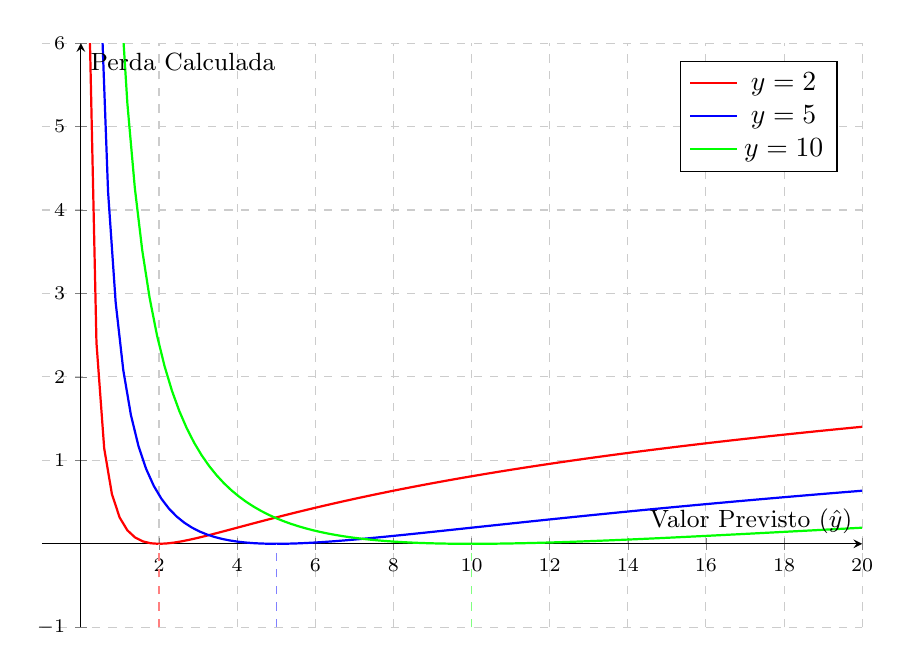
\begin{tikzpicture}
        \begin{axis}[
            xlabel={Valor Previsto ($\hat{y}$)},
            ylabel={Perda Calculada},
            axis lines=middle,
            grid=major,
            grid style={dashed, gray!40},
            xmin=-1, xmax=20,
            ymin=-1, ymax=6,  % Ajustado para melhor visualização da Gamma
            legend pos=north east, % Movido para um local melhor
            width=12cm,
            height=9cm,
            title style={font=\bfseries},
            label style={font=\small},
            tick label style={font=\scriptsize}
        ]
            % Fórmula: ln(x/y) + (y/x) - 1
            
            % Curva para y=2
            \addplot[domain=0.2:20, samples=101, color=red, thick] {ln(x/2) + (2/x) - 1};
            \addlegendentry{$y=2$}
            % Mínimo em y=2, perda=0
            \draw[dashed, red!50] (axis cs:2, -1) -- (axis cs:2, 0);

            % Curva para y=5
            \addplot[domain=0.5:20, samples=101, color=blue, thick] {ln(x/5) + (5/x) - 1};
            \addlegendentry{$y=5$}
            % Mínimo em y=5, perda=0
            \draw[dashed, blue!50] (axis cs:5, -1) -- (axis cs:5, 0);

            % Curva para y=10
            \addplot[domain=1:20, samples=101, color=green, thick] {ln(x/10) + (10/x) - 1};
            \addlegendentry{$y=10$}
            % Mínimo em y=10, perda=0
            \draw[dashed, green!50] (axis cs:10, -1) -- (axis cs:10, 0);
            
        \end{axis}
    \end{tikzpicture}
    \caption{Gráfico da Perda Gamma para diferentes valores reais de $y$. O mínimo de cada curva (Perda = 0) ocorre em $\hat{y}=y$.}%
    \label{fig:gamma-loss}
    \fonte{O autor (2025).}
\end{figure}

\subsubsection*{Características da perda gamma}

\begin{description}[style=sameline, leftmargin=1.5em, font=\bfseries\color{black}] 
    \item[Característica 1] 
    \item[característica 2] 
    \item[Característica 3] 
\end{description}

\subsubsection*{Gradiente da perda Gamma}

\begin{equacaodestaque}{Derivada da perda gamma}
    \frac{\partial\Loss_{\text{Gamma}}}{\partial\hat{y}_j} = \frac{1}{\hat{y}_j} -\frac{y_j}{\hat{y}_j^2} = \frac{\hat{y}_j -y_j}{\hat{y}_j^2}%
    \label{eq:gamma-loss-derivada}
\end{equacaodestaque}

\begin{figure}[h!]
    \centering
    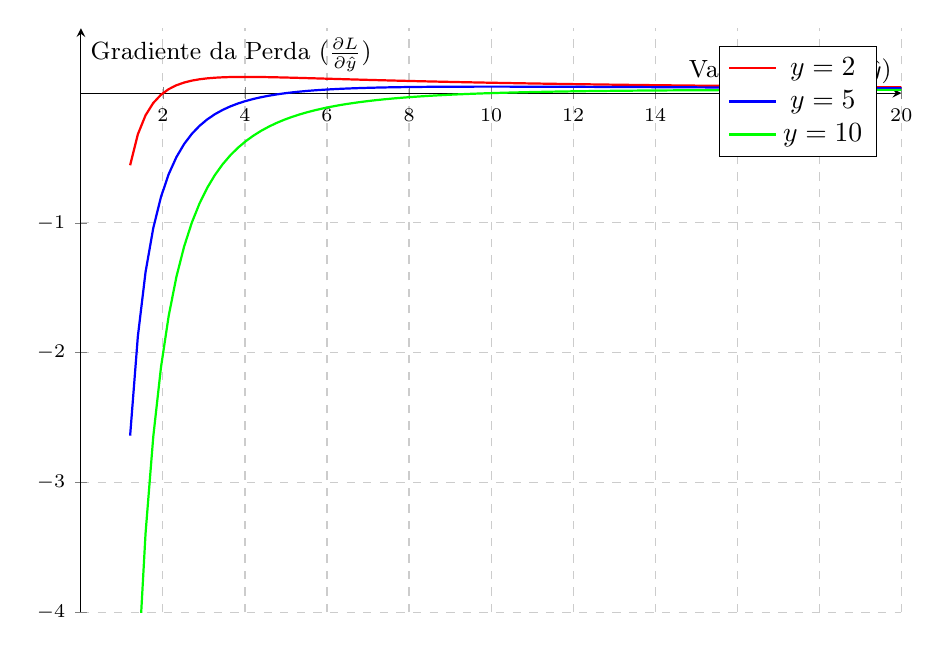
\begin{tikzpicture}
        \begin{axis}[
            xlabel={Valor Previsto ($\hat{y}$)},
            ylabel={Gradiente da Perda ($\frac{\partial L}{\partial \hat{y}}$)},
            axis lines=middle,
            grid=major,
            grid style={dashed, gray!40},
            xmin=0, xmax=20,  % Ajustado para a derivada da Gamma
            ymin=-4, ymax=0.5,   % Ajustado para a derivada da Gamma
            legend pos=north east, % Movido para um local melhor
            width=12cm,
            height=9cm,
            title style={font=\bfseries},
            label style={font=\small},
            tick label style={font=\scriptsize}
        ]
            % Fórmula: (x - y) / (x^2)
            
            % Curva para y=2
            \addplot[domain=1.2:20, samples=101, color=red, thick] {(x - 2) / (x^2)};
            \addlegendentry{$y=2$}
            
            % Curva para y=5
            \addplot[domain=1.2:20, samples=101, color=blue, thick] {(x - 5) / (x^2)};
            \addlegendentry{$y=5$}

            % Curva para y=10
            \addplot[domain=1.2:20, samples=101, color=green, thick] {(x - 10) / (x^2)};
            \addlegendentry{$y=10$}
            
        \end{axis}
    \end{tikzpicture}
    \caption{Gráfico da derivada da Perda Gamma. O gradiente é zero quando $\hat{y}=y$ e assintótico a 0 para $\hat{y} \to \infty$.}%
    \label{fig:gamma-loss-derivada}
    \fonte{O autor (2025).}
\end{figure}

\subsubsection*{Aplicações da perda gamma em aprendizado de máquina}%
\index{Aplicações práticas! Deviância Gamma}

\begin{description}[style=sameline, leftmargin=1.5em, font=\bfseries\color{black}] 
    \item[Aplicação 1 (Área):] 
    \item[Aplicação 2 (Área):] 
    \item[Aplicação 3 (Área):] 
\end{description}

\subsection{Perda de Tweedie (Tweedie Loss)}%
\index{Funções de Perda!Perda de Tweedie (\textit{Tweedie Loss})}

\begin{equacaodestaque}{Perda de Tweedie (\textit{Tweedie Loss})}
    \Loss_{\text{Tweedie}}(y_j, \hat{y}_j; p) = -\frac{y_j \cdot \hat{y}_j^{1-p}}{1-p} + \frac{\hat{y}_j^{2-p}}{2-p}%
    \label{eq:tweedie-loss}
\end{equacaodestaque}

Em que:

\begin{description}[style=sameline, leftmargin=1.5em, font=\bfseries\color{black}]  
    \item[$y_j$] representa o valor real da j-ésima amostra;
    \item[$\hat{y}_j$] representa o valor predito pelo modelo;
    \item[$N$] representa o número de amostras.
\end{description}

\begin{figure}[h!]
    \centering
    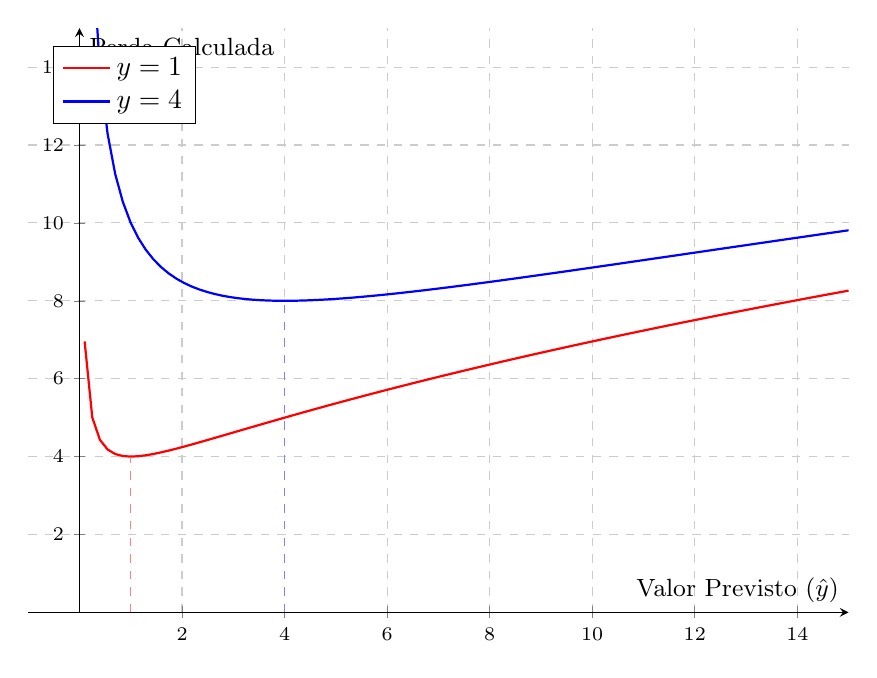
\begin{tikzpicture}
        \begin{axis}[
            xlabel={Valor Previsto ($\hat{y}$)},
            ylabel={Perda Calculada},
            axis lines=middle,
            grid=major,
            grid style={dashed, gray!40},
            xmin=-1, xmax=15,
            ymin=0, ymax=15,
            legend pos=north west,
            width=12cm,
            height=9cm,
            title style={font=\bfseries},
            label style={font=\small},
            tick label style={font=\scriptsize}
        ]
            % Definição do parâmetro p
            \def\p{1.5}

            % Curva para y=1
            \addplot[domain=0.1:15, samples=101, color=red, thick] 
                { -1*x^(1-\p)/(1-\p) + x^(2-\p)/(2-\p) };
            \addlegendentry{$y=1$}
            \draw[dashed, red!50] (axis cs:1, 0) -- (axis cs:1, {-1*1^(1-\p)/(1-\p) + 1^(2-\p)/(2-\p)});

            % Curva para y=4
            \addplot[domain=0.1:15, samples=101, color=blue, thick] 
                { -4*x^(1-\p)/(1-\p) + x^(2-\p)/(2-\p) };
            \addlegendentry{$y=4$}
            \draw[dashed, blue!50] (axis cs:4, 0) -- (axis cs:4, {-4*4^(1-\p)/(1-\p) + 4^(2-\p)/(2-\p)});
            
        \end{axis}
    \end{tikzpicture}
    \caption{Gráfico da Perda de Tweedie para $p=1.5$. O mínimo de cada curva ocorre em $\hat{y}=y$.}%
    \label{fig:tweedie-loss}
    \fonte{O autor (2025).}
\end{figure}

\subsubsection*{Características da Perda de Tweedie}

\begin{description}[style=sameline, leftmargin=1.5em, font=\bfseries\color{black}] 
    \item[Característica 1:] 
    \item[Característica 2:] 
    \item[Característica 3:] 
\end{description}

\subsubsection*{Gradiente da perda de Tweedie}

\begin{equacaodestaque}{Derivada da Perda de Tweedie}
    \frac{\partial\Loss_{\text{Tweedie}}}{\partial\hat{y}_j} = \hat{y}_j^{-p}(\hat{y}_j -y_j)%
    \label{eq:tweedie-loss-derivada}
\end{equacaodestaque}

\begin{figure}[h!]
    \centering
    \begin{tikzpicture}
        \begin{axis}[
            xlabel={Valor Previsto ($\hat{y}$)},
            ylabel={Gradiente da Perda ($\frac{\partial L}{\partial \hat{y}}$)},
            axis lines=middle,
            grid=major,
            grid style={dashed, gray!40},
            xmin=-1, xmax=15,
            ymin=-2, ymax=1.5,
            legend pos=south east,
            width=12cm,
            height=9cm,
            title style={font=\bfseries},
            label style={font=\small},
            tick label style={font=\scriptsize}
        ]
            % Definição do parâmetro p
            \def\p{1.5}
            
            % Curva para y=1
            \addplot[domain=0.2:15, samples=101, color=red, thick] 
                {x^(-\p)*(x-1)};
            \addlegendentry{$y=1$}
            
            % Curva para y=4
            \addplot[domain=0.2:15, samples=101, color=blue, thick] 
                {x^(-\p)*(x-4)};
            \addlegendentry{$y=4$}

            % Linhas verticais onde o gradiente é zero
            \draw[dashed, red!50] (axis cs:1, -2) -- (axis cs:1, 1.5);
            \draw[dashed, blue!50] (axis cs:4, -2) -- (axis cs:4, 1.5);
            
        \end{axis}
    \end{tikzpicture}
    \caption{Gráfico da derivada da Perda de Tweedie para $p=1.5$. O gradiente é zero quando a previsão é igual ao valor real.}%
    \label{fig:tweedie-loss-derivada}
    \fonte{O autor (2025).}
\end{figure}

\subsubsection*{Algumas Aplicações da Perda de Tweedie}%
\index{Aplicações práticas! Perda de Tweedie}

\begin{description}[style=sameline, leftmargin=1.5em, font=\bfseries\color{black}] 
    \item[Aplicação 1 (Área):] 
    \item[Aplicação 2 (Área):] 
    \item[Aplicação 3 (Área):] 
\end{description}

\section{Comparativo: Funções de Perda para Regressão}

\begin{table}[htbp]
    \centering
    \begin{threeparttable}
        \caption{Comparativo das funções das funções de perda para problemas de regressão}%
        \label{tab:comparativo-funcoes-de-perda-para-regressao}

        \begin{tabularx}{\textwidth}{p{3.2cm} *{1}{>{\raggedright\arraybackslash}X}}
            \toprule
            \textbf{Função} & \textbf{Principais características} \\
            \midrule
            Erro quadrático médio (MSE) & -  \\
            \addlinespace
            Erro absoluto médio (MAE) & - \\
            \addlinespace
            Perda de Huber (\textit{Huber loss}) & - \\
            \addlinespace
            Perda log-cosh (\textit{Log-cosh loss}) & - \\
            \addlinespace
            Erro quadrático logarítmico médio (MSLE) & - \\
            \addlinespace
            Perda quantílica (\textit{Quantile loss}) & - \\
            \addlinespace
            Perda epsilon-insensível (\textit{$\epsilon$-insentive}) & - \\
            \addlinespace
            Perda de Poisson (\textit{Poisson loss}) & - \\
            \addlinespace
            Deviância Gamma (\textit{Poisson loss}) & - \\
            \addlinespace
            Perda de Tweedie (\textit{Tweedie loss}) & - \\
            \addlinespace
        \end{tabularx}
        
        \begin{tablenotes}[para]
            \small
            \item[] Fonte: O autor (2025).
        \end{tablenotes}

    \end{threeparttable}
\end{table}

\section{Fluxograma: Escolhendo a Função de Perda Ideal}

\medskip
\begin{center}
 * * *
\end{center}
\medskip

\subsubsection*{Indo Além das Funções de Perda Para Regressão}

Nesse capítulo foi visto uma série de funções de perdas que tinham uma característica em comum: são utilizadas para lidar com problemas de regressão. Contudo, esse não é o único conjunto de funções de perda que existe. Existem funções de perda que são ideais para problemas de classificação, seja ele com duas classes (binário), ou multi-classe, essas funções são o tópico central do Capítulo~\ref{cap:perda-classificacao}. Além disso, existem vários outros tipos de problemas, alguns bem mais específicos, como reconhecer objetos em uma foto. Dessa forma, o Capítulo~\ref{cap:perdas-especificas} busca fazer uma coletânea de outras funções de perda para situações mais específicas ao se construir um modelo de aprendizado de máquina.

Contudo, foram vistas apenas as funções de perda, e foi visto também que algumas podem servir como métricas, indicando de forma mais simples e direta se o modelo está performando bem ou não. Assim, um complemento para esse capítulo agora que você leitor conhece as funções de perda para regressão, é ler também o capítulo seguinte a este, o Capítulo~\ref{cap:metricas-de-avaliacao-para-regressao}. Ele é dedicado a explicar diferentes métricas que podem ser utilizadas para avaliar um modelo de regressão. De forma que será possível conhecer não só a função de perda ideal, mas também o conjunto de métricas ideais para avaliar o modelo desenvolvido.

\medskip
\begin{center}
 * * *
\end{center}
\medskip
